% LaTeX file for Chapter 03














\chapter{Results}



% \begin{table}
% 
% \caption{Comparison of confidence intervals for the mean differences across scenarios. The first row of each pair corresponds to the confidence interval from the linear model (lm), while the second row corresponds to the bootstrap method.}
% \centering
% \begin{tabular}[t]{lrr}
% \toprule
%   & Lower Bound & Upper Bound\\
% \midrule
% Scenario 1 (lm) & -0.58231 & -0.54359\\
% Scenario 1 (bootstrap) & -0.58210 & -0.54355\\
% Scenario 2 (lm) & -0.59118 & -0.55371\\
% Scenario 2 (bootstrap) & -0.59091 & -0.55405\\
% Scenario 3 (lm) & -0.06784 & -0.02799\\
% \addlinespace
% Scenario 3 (bootstrap) & -0.06784 & -0.02752\\
% \bottomrule
% \end{tabular}
% \end{table}


\section{Experiment 1: TRAM-DAG (simulation study)}

In this section, we present the results of a simulation study to evaluate the performance of the TRAM-DAG model in a simple scenario as illustrated by the DAG in Figure \ref{fig:dag_and_matrix}. The model was fitted on synthetic data. Figure \ref{fig:exp1_loss_parameters} shows the loss and the estimated parameters for the linear shifts over epochs during training. The loss is minimized during training and the estimated parameters $\beta_{12}$ and $\beta_{13}$ converge to the true values used in the DGP. The linear shift parameters are interpretable part of the model (log odds ratios). 
From the fitted model, we generated samples from the observational distribution, as shown in Figure \ref{fig:exp1_observational_distribution}. Then we drew samples from the interventional distribution, where $X_2 = 1$ is fixed, as shown in Figure \ref{fig:exp1_interventional_distribution}. Fixing $X_2$ leads to a distributional change in $X_3$. The TRAM-DAG model learns the linear shifts ($\beta_{12}$, $\beta_{13}$) and the complex shift ($\text{CS}(X_2)$), which are shown in Figure \ref{fig:exp1_shifts}. Figure \ref{fig:exp1_intercepts} presents the intercepts learned for each of the nodes, with the estimates by the continuous outcomes logistic regression (Colr() function from tram-package \citep{hothorn2018}) function as comparison for the continuous variables and the true values used in the DGP for ordinal variable X3 (3 cut points needed for the 4 levels). Finally, Figure \ref{fig:exp1_counterfactuals} shows the counterfactuals estimated by the TRAM-DAG model for varying values of $X_1$. The counterfactuals are the predicted values of $X_2$ if $X_1$ would have taken other values instead of the observed value. 

\begin{figure}[htbp]
\centering
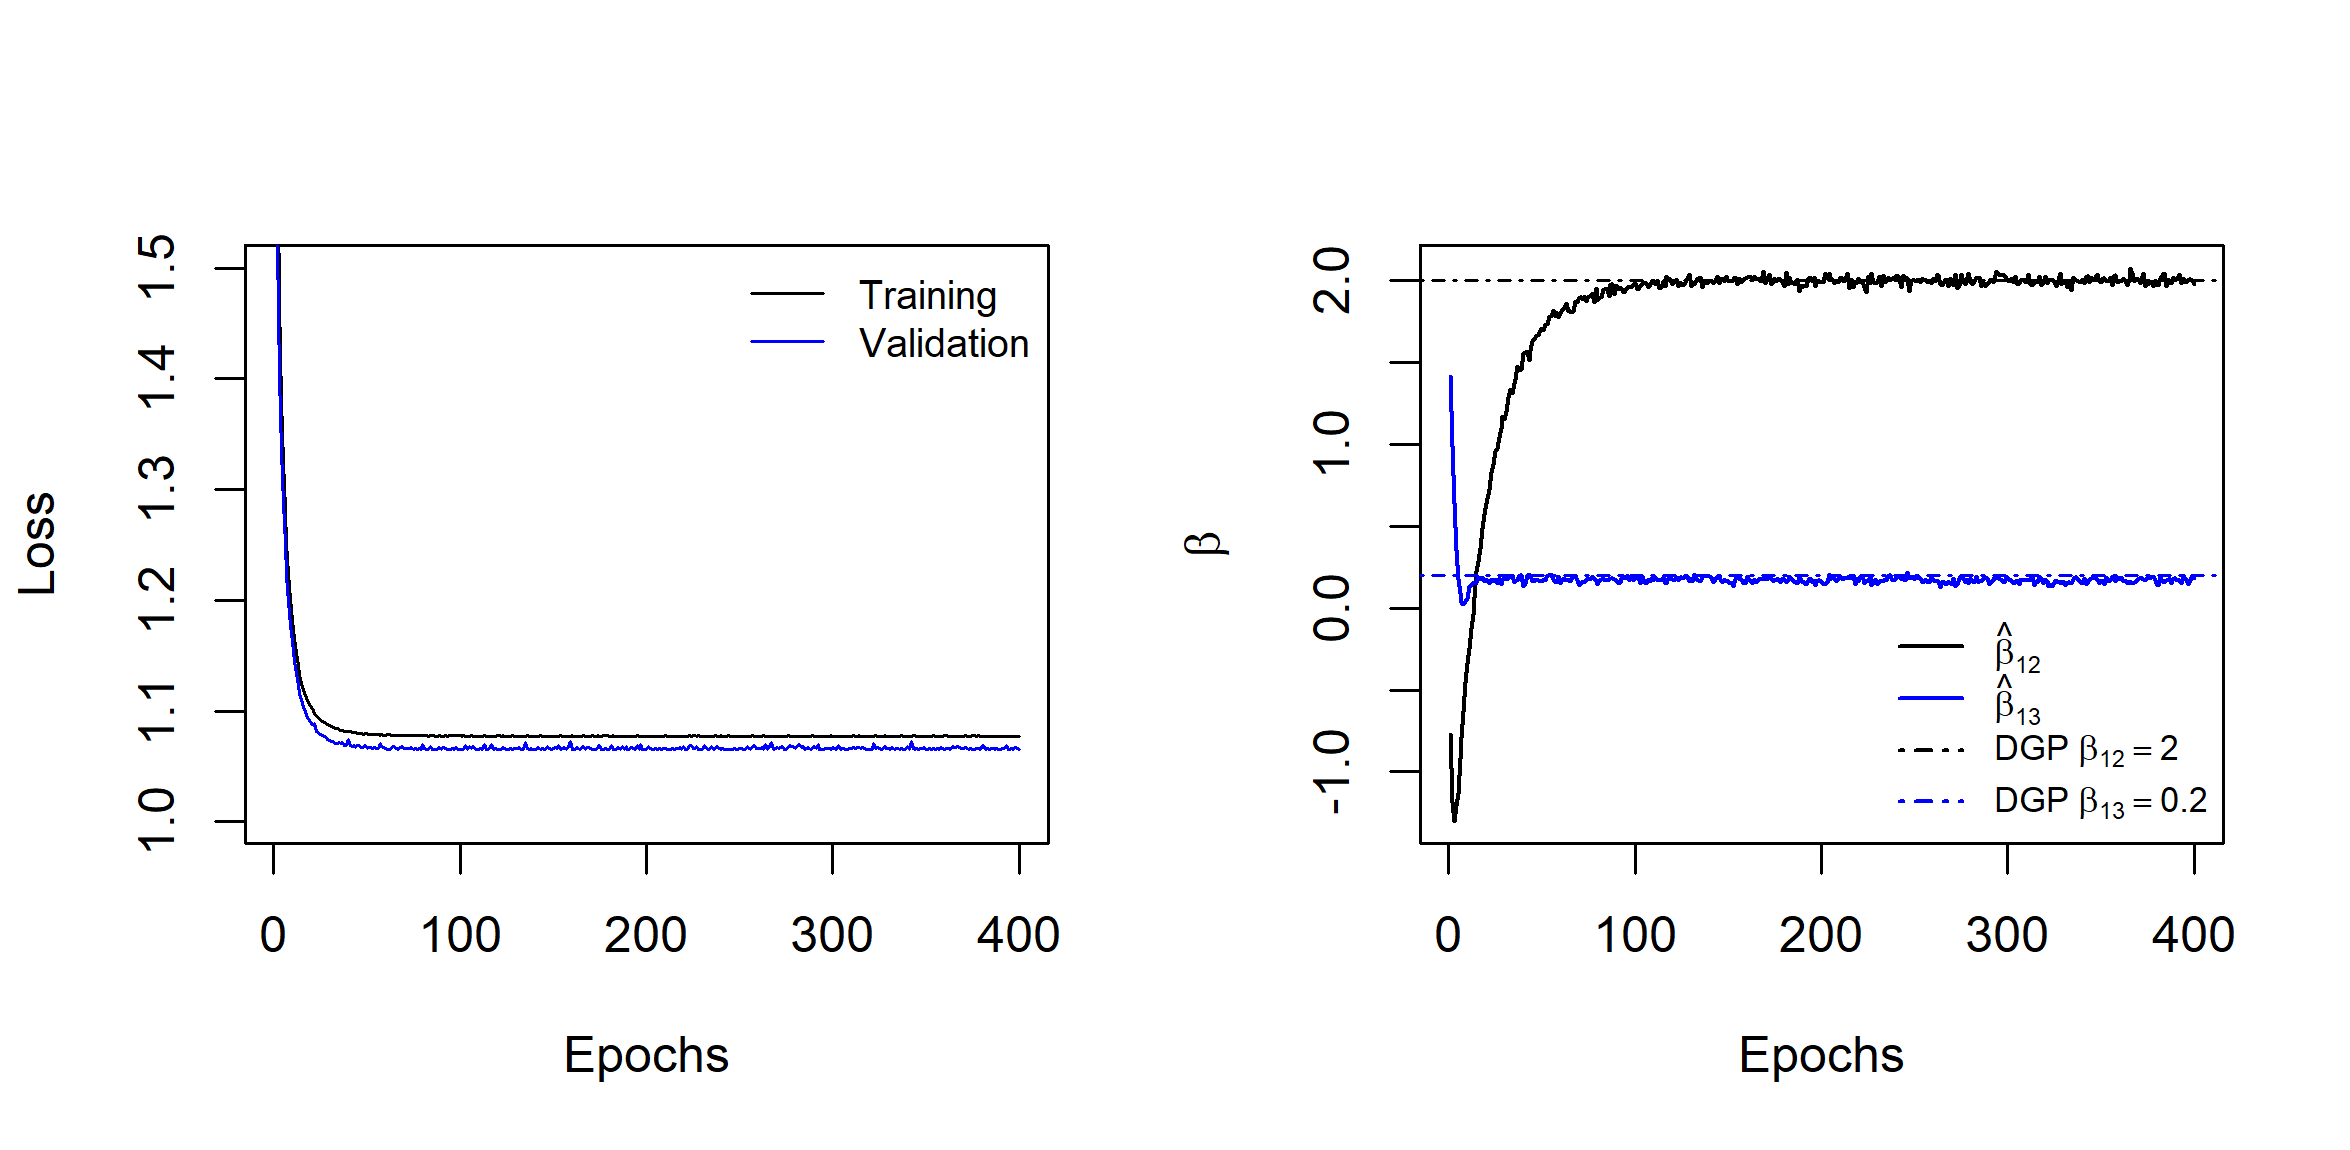
\includegraphics[width=0.9\textwidth]{img/exp1_loss_parameters.png}
\caption{TRAM-DAG model fitting over 400 epochs for experiment 1. Left: Loss functions on the training set and a separate validation set; Right: Estimated parameters (betas) for the linear shift components over epochs. They converge to the true values.}
\label{fig:exp1_loss_parameters}
\end{figure}



\begin{figure}[htbp]
\centering
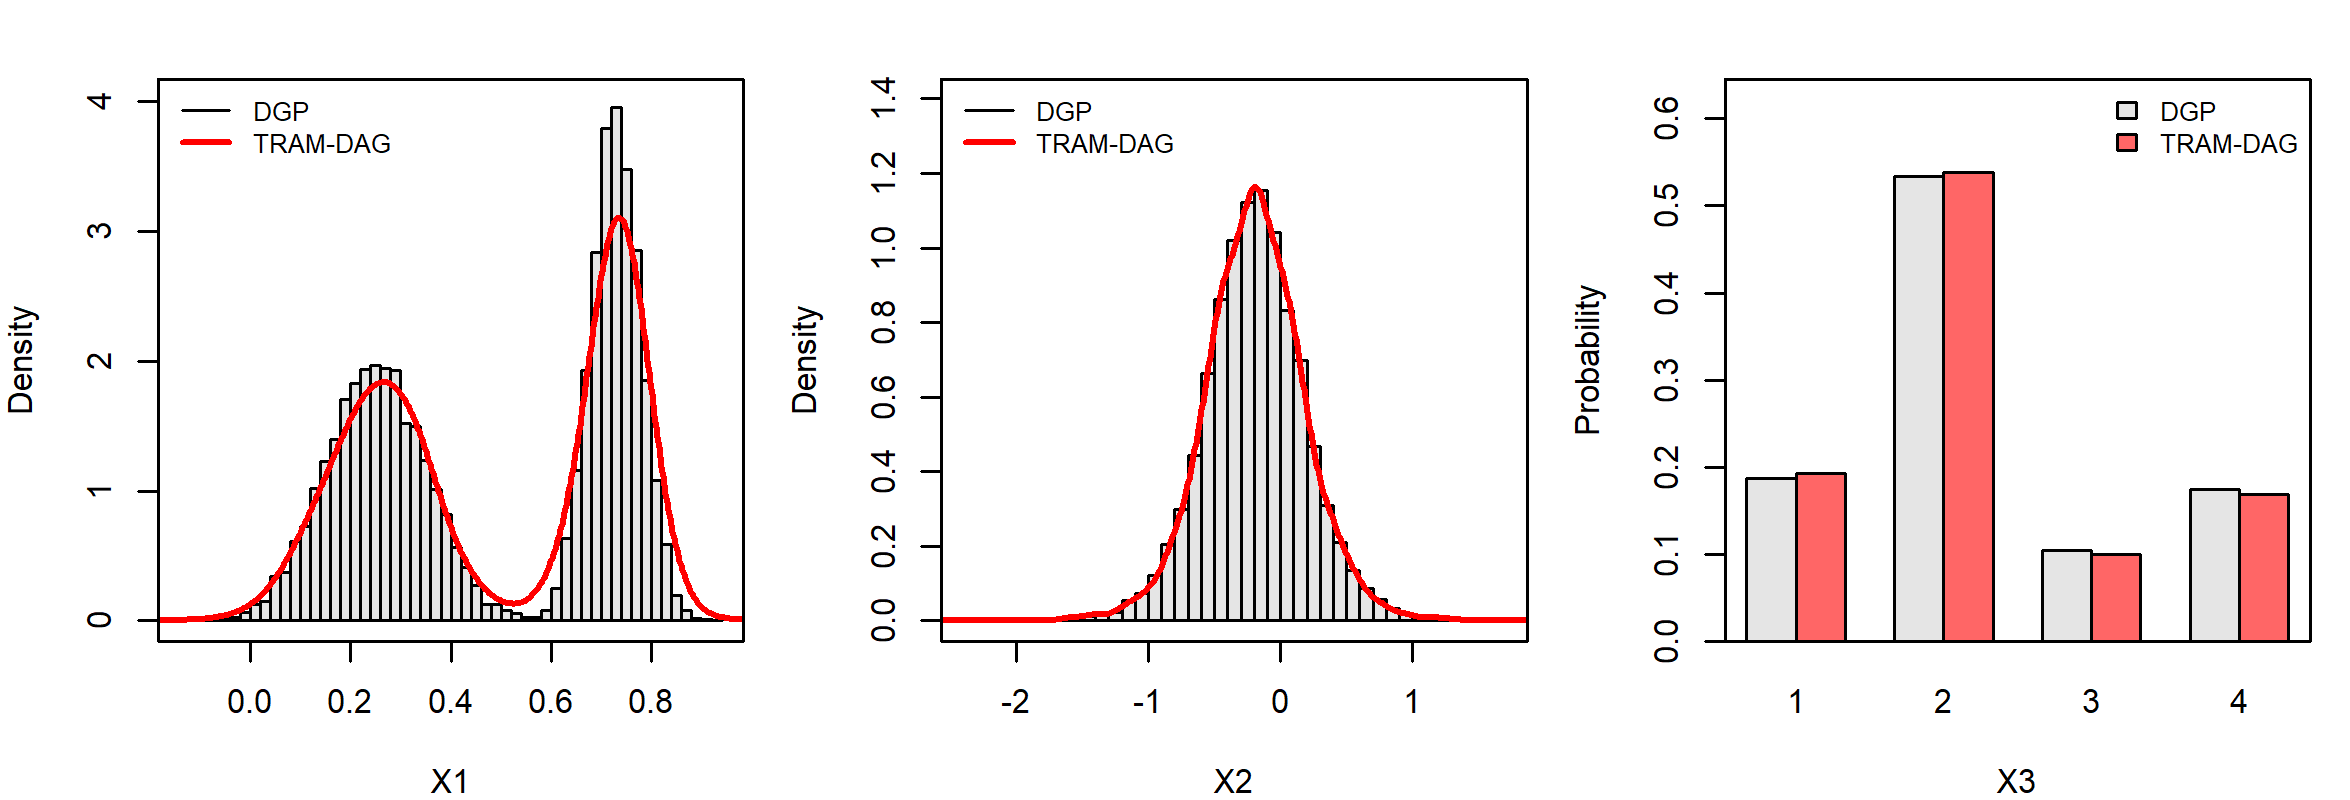
\includegraphics[width=0.9\textwidth]{img/exp1_observational_distribution.png}
\caption{Samples by the TRAM-DAG generated from the learned observational against the true observations from the DGP.}
\label{fig:exp1_observational_distribution}
\end{figure}




\begin{figure}[htbp]
\centering
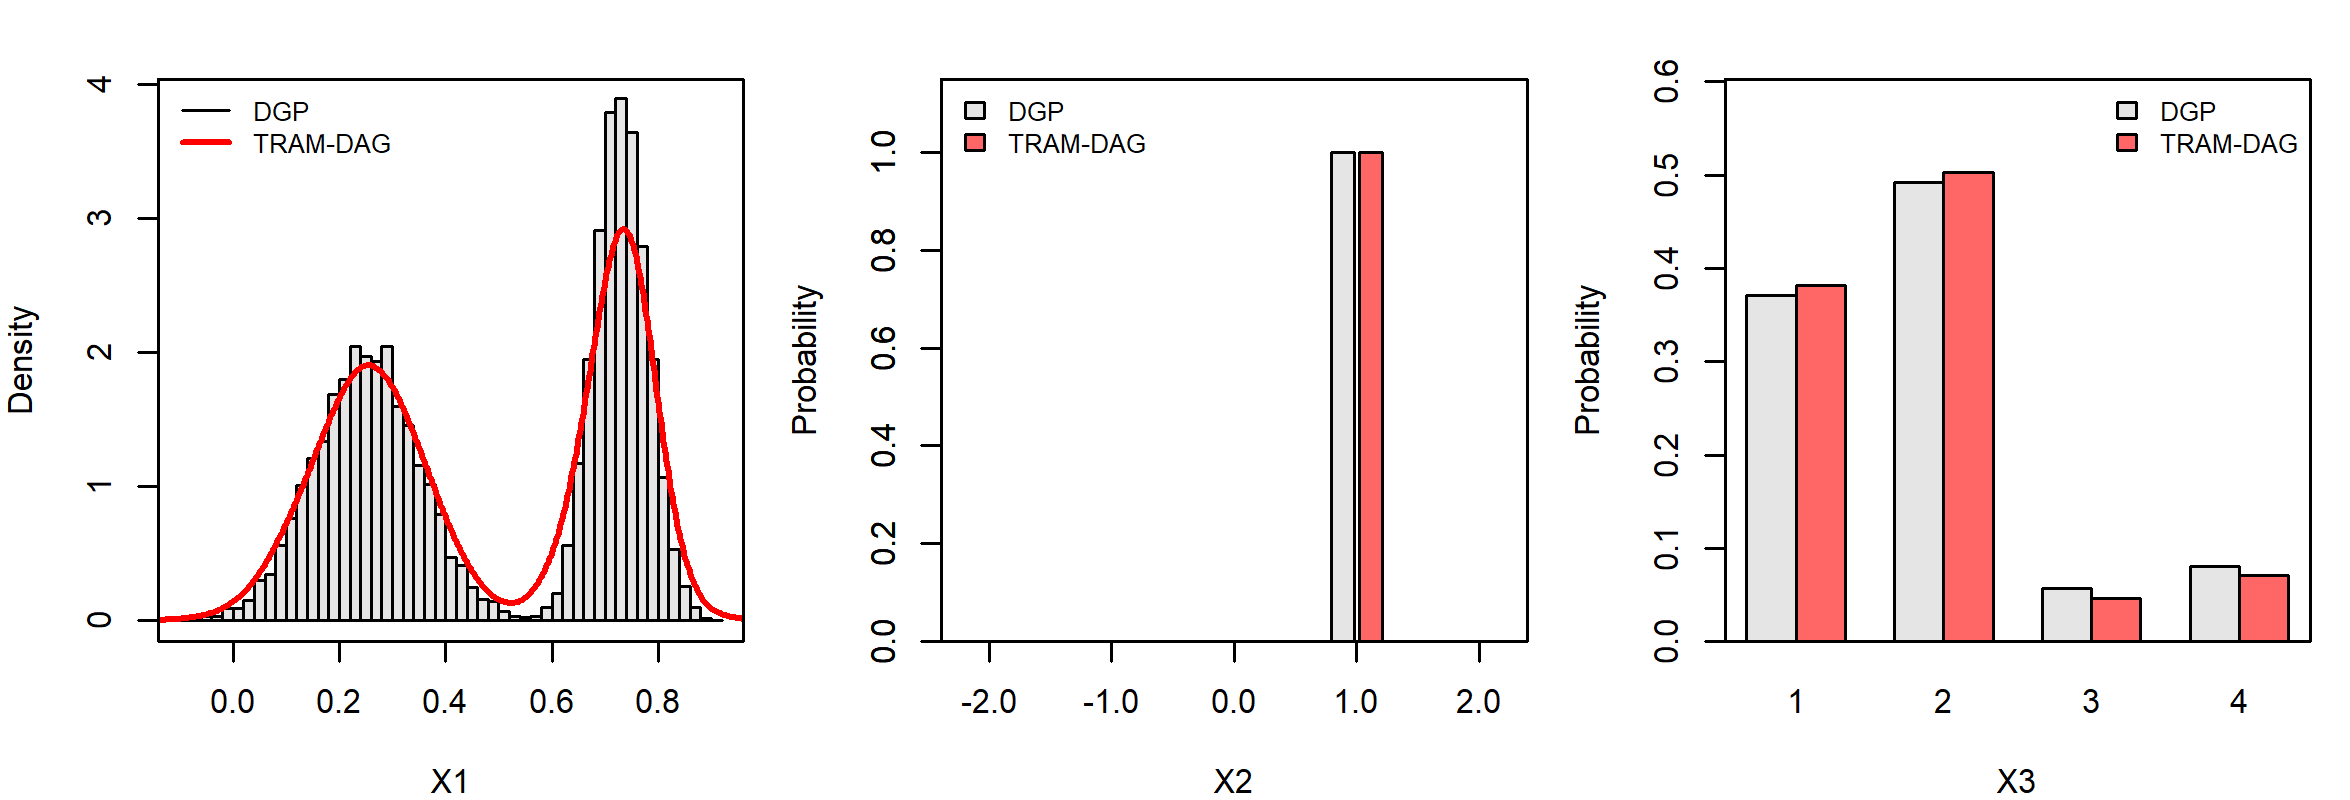
\includegraphics[width=0.9\textwidth]{img/exp1_interventional_distribution.png}
\caption{Samples by the TRAM-DAG generated against the true observations from the interventional distribution, where $X_2 = 1$ is fixed. According to the DAG, this affects a distributional change in $X_3$.}
\label{fig:exp1_interventional_distribution}
\end{figure}



\begin{figure}[htbp]
\centering
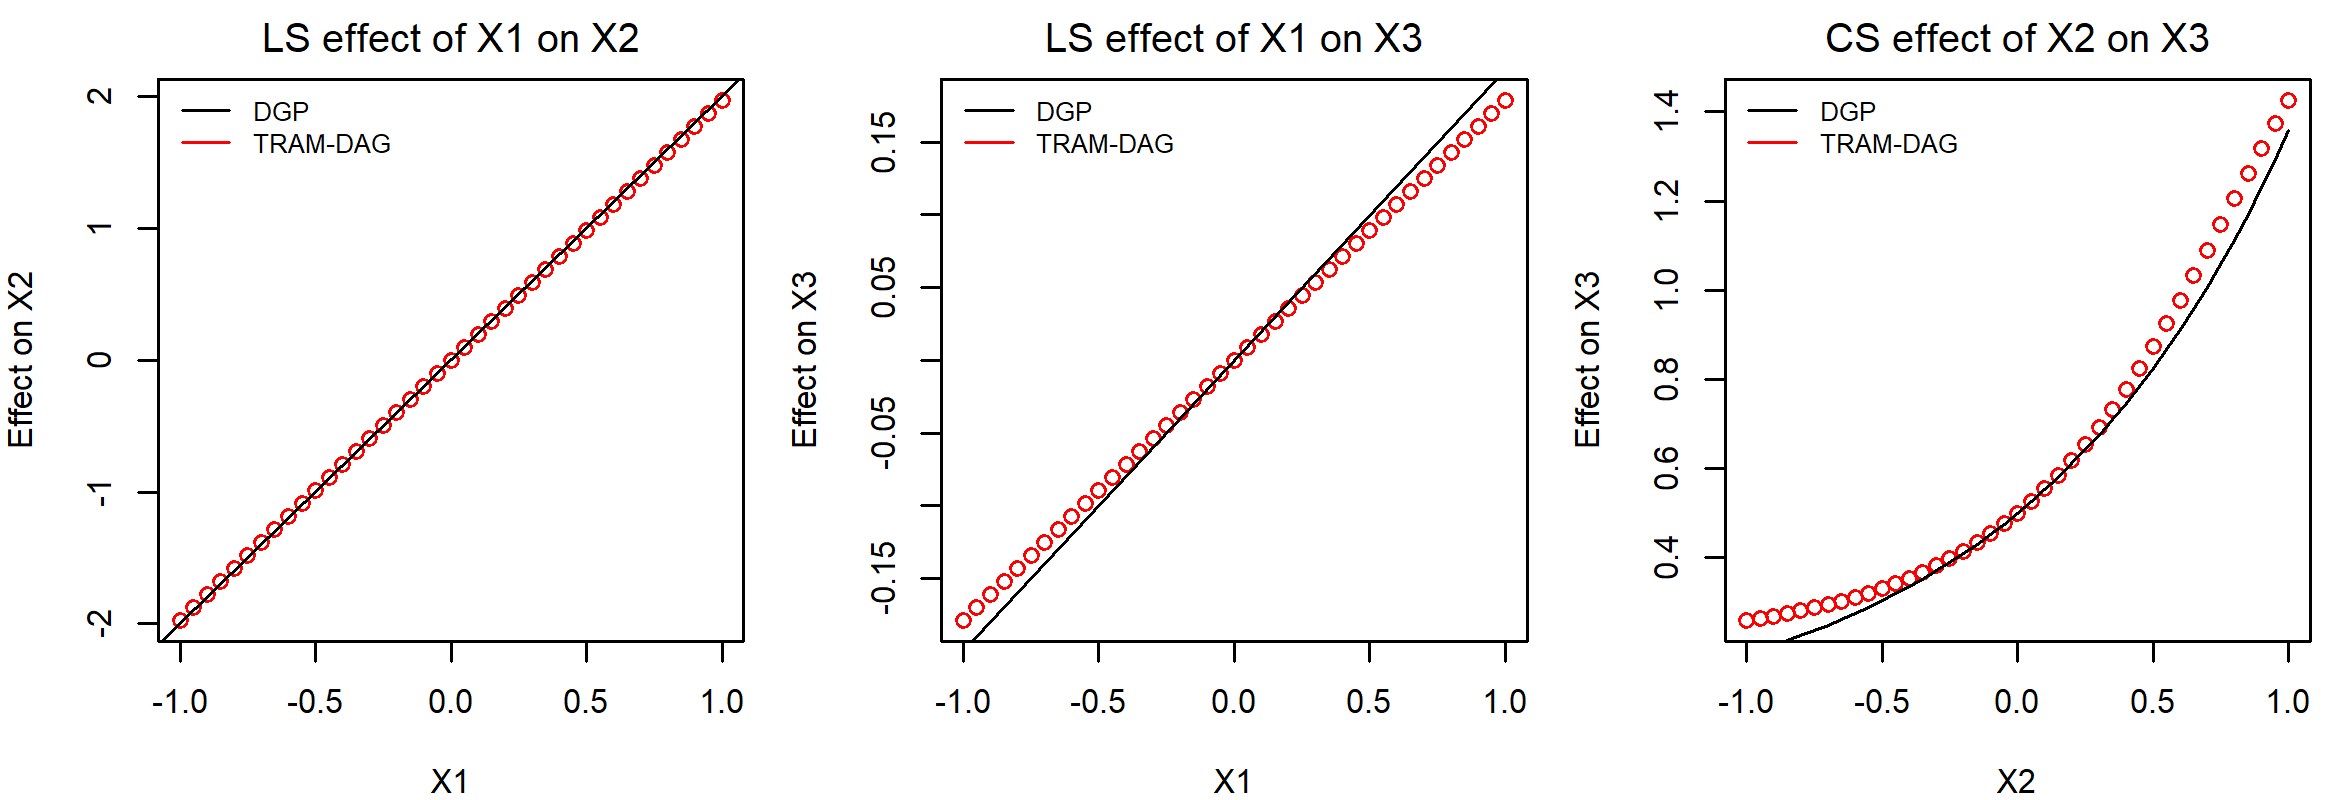
\includegraphics[width=0.9\textwidth]{img/exp1_LS_CS.png}
\caption{Linear shift and complex shift learned by the TRAM-DAG. Left: LS($X_1$) on $X_2$; Middle: LS($X_1$) on $X_3$; Right: CS($X_2$) on $X_3$. For visualization, we subtracted $\delta_0 = \text{CS}(0) - f(0)$ from the estimated complex shift CS(X2) to make it comparable to the DGP shift $f(X_2)$}
\label{fig:exp1_shifts}
\end{figure}



\begin{figure}[htbp]
\centering
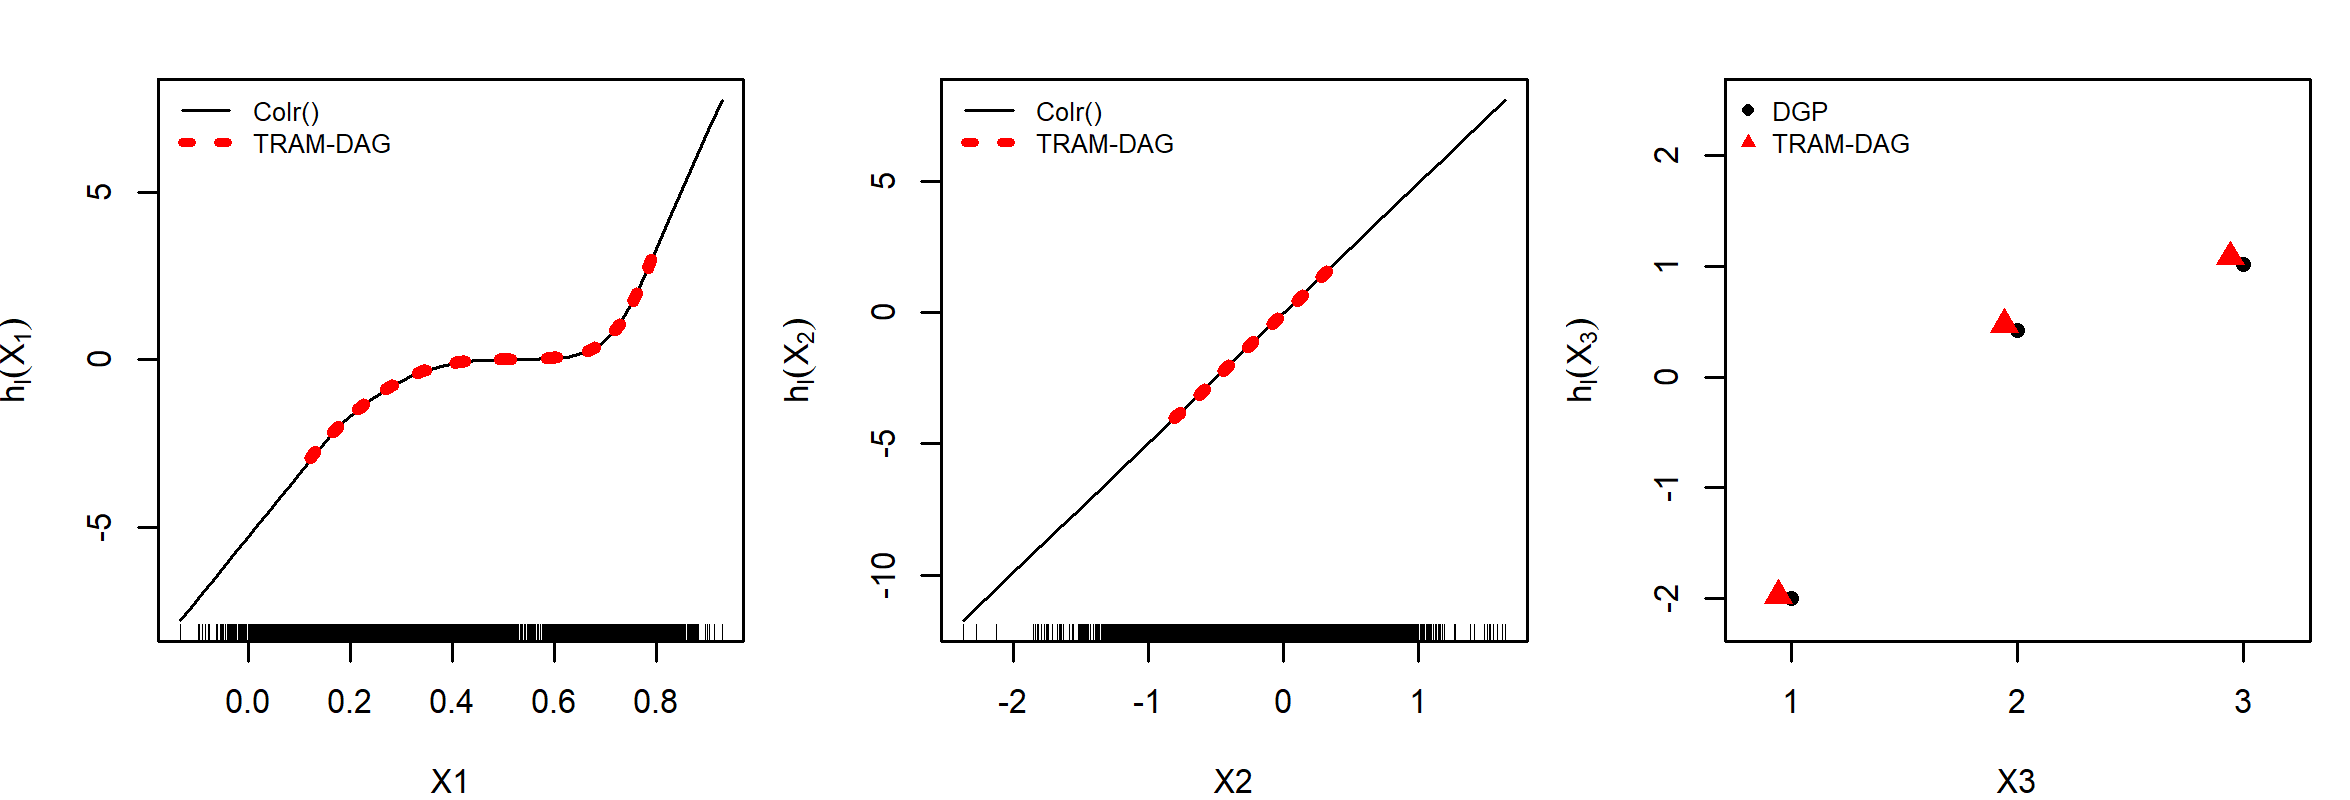
\includegraphics[width=0.9\textwidth]{img/exp1_baseline_trafo.png}
\caption{Intercepts learned for each of the nodes, with the estimates by the Colr() function for the continuous variables and the true values used in the DGP for ordinal X3. Left: smooth baseline transformation function for continuous X1; Middle: smooth baseline transformation function for continuous X2 ; Right: cut-points as the baseline transformation function for ordinal X3. For the last plot we added $\delta_0 = \text{CS}(0) - f(0)$ to the estimated cut-offs to make them comparable to the true parameters from the DGP.}
\label{fig:exp1_intercepts}
\end{figure}





\begin{figure}[htbp]
\centering
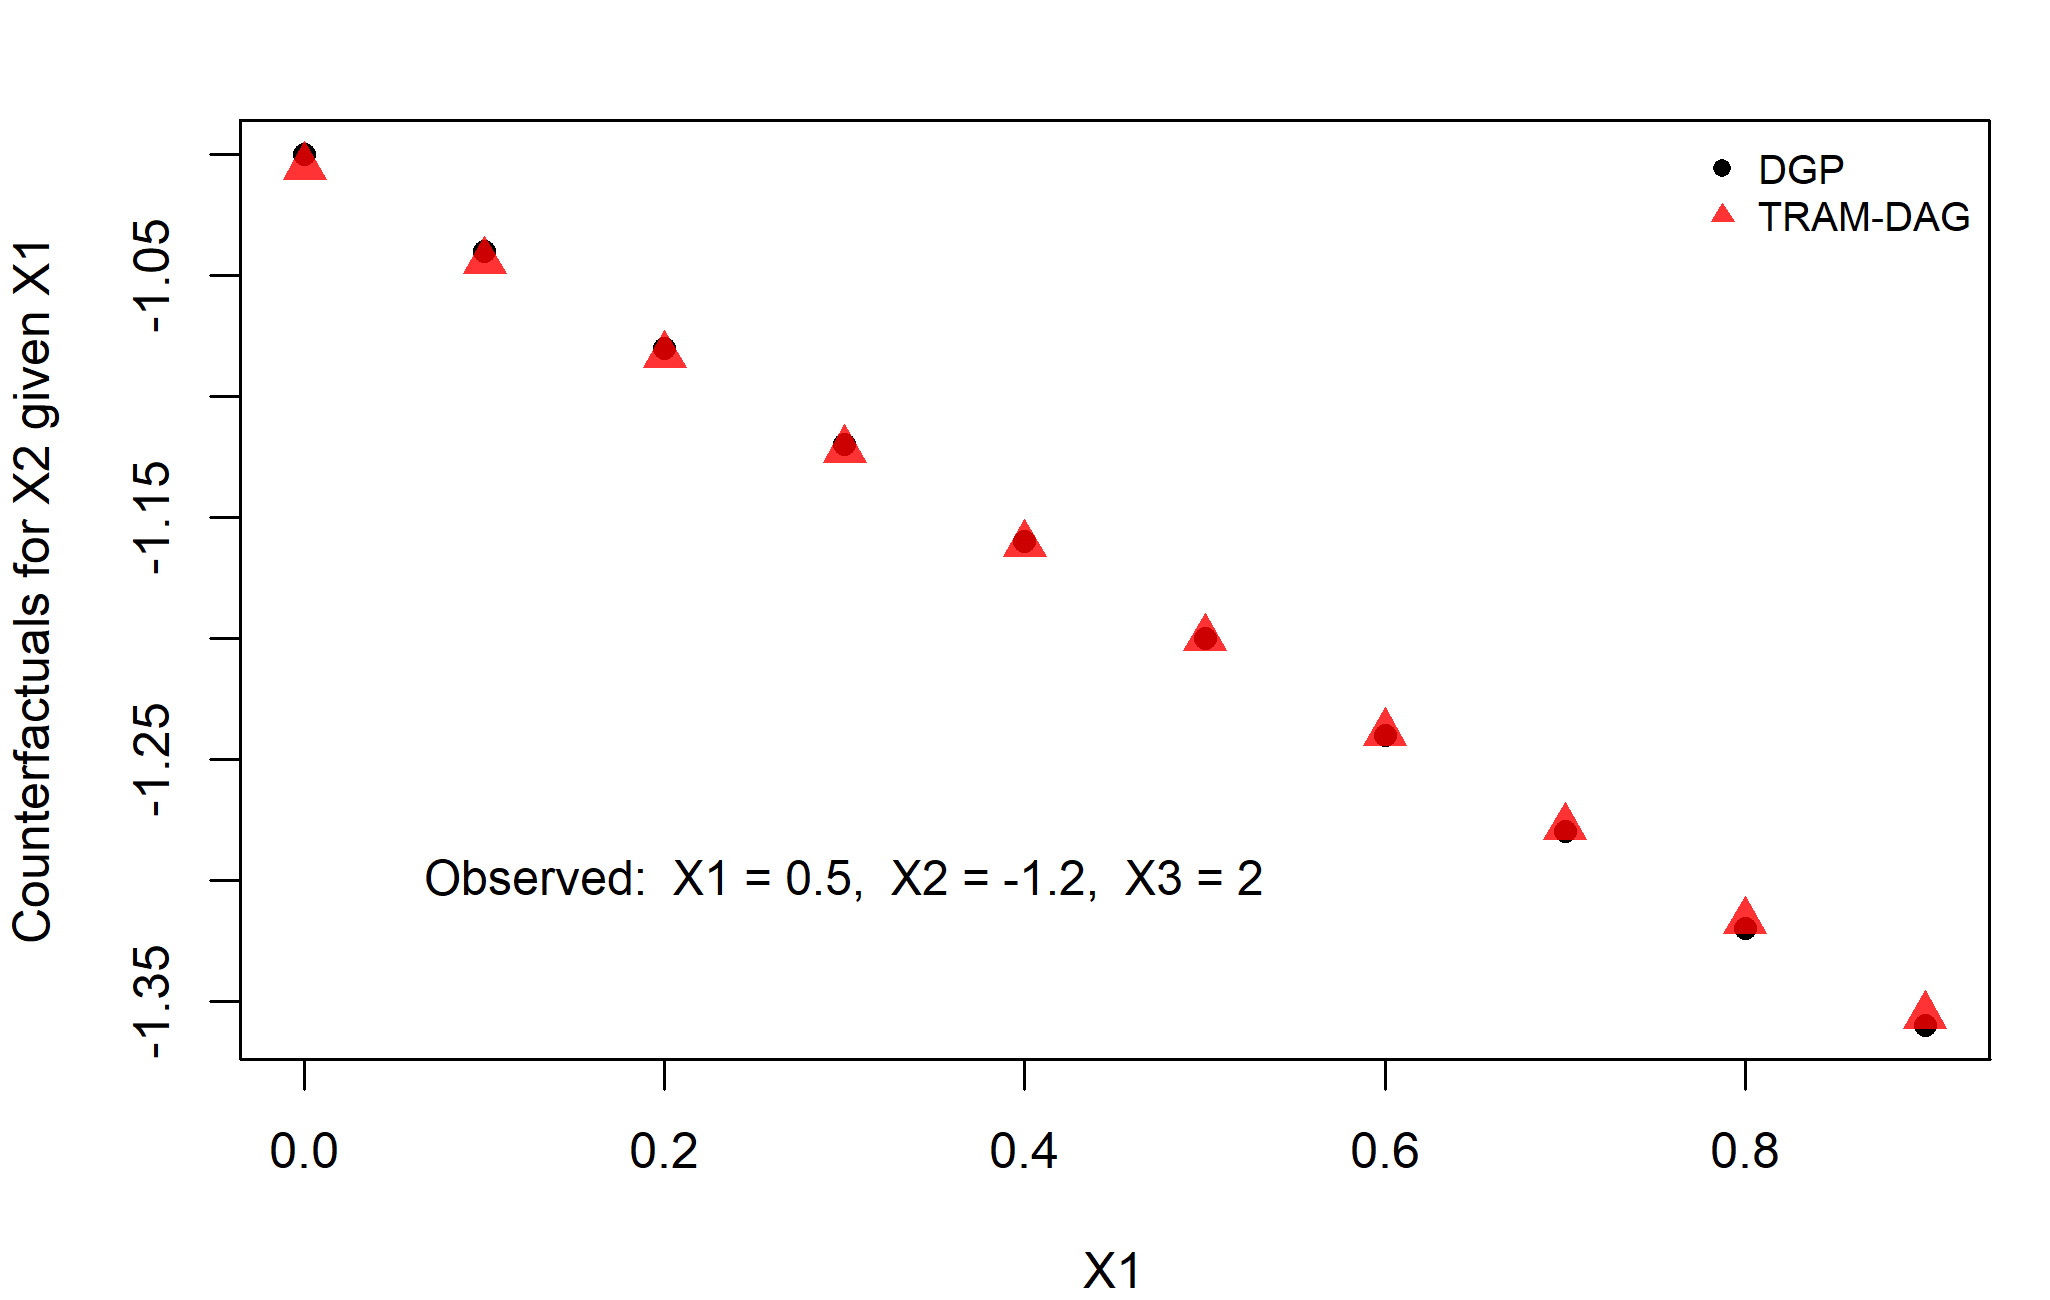
\includegraphics[width=0.9\textwidth]{img/exp1_counterfactuals.png}
\caption{Counterfactuals for $X_2$ estimated with the TRAM-DAG for varying $X_1$. We assumed observations $X_1 = 0.5$, $X_2 = -1.2$, $X_3 = 2$ and determined the counterfactual values for $X_2$ if $X_1$ would have taken other values instead of the observed value.}
\label{fig:exp1_counterfactuals}
\end{figure}


\clearpage


\section{Experiment 2: ITE on International Stroke Trial (IST)} \label{sec:results_experiment2}


In this section, we present the results of the ITE estimation on the International Stroke Trial (IST) dataset. The observed treatment effect $\text{P}(Y=1|T=1) - \text{P}(Y=1|T=0)$ on the training set was -2.4\% absolute risk reduction with a 95\% confidence interval of -4.1\% to -0.6\%. The observed treatment effect on the test set was -0.1\% with a 95\% confidence interval of -2.6\% to 2.3\%. The estimated ITEs were computed using three different models: the T-learner logistic regression, the T-learner tuned random forest, and the S-learner TRAM-DAG. The estimated average treatment effect on the test set as $\text{ATE}_\text{pred}=\text{mean}(\text{ITE}_\text{pred})$ was -2.5\% for the T-learner logistic regression, -2.2\% for the T-learner tuned random forest, and -3.1\% for the S-learner TRAM-DAG. The density of estimated ITEs and ITE-ATE plots in terms of risk difference per estimated ITE subgroup are presented in Figures \ref{fig:IST_density_ITE_ATE_glm_tlearner} - \ref{fig:IST_density_ITE_ATE_TRAM_DAG}. Calibration plots are shown in the Appendix \ref{sec:calibrations_experiment2}, Figures \ref{fig:calibration_IST_glm} - \ref{fig:calibration_IST_TRAM_DAG}. 






\begin{figure}[htbp]
\centering
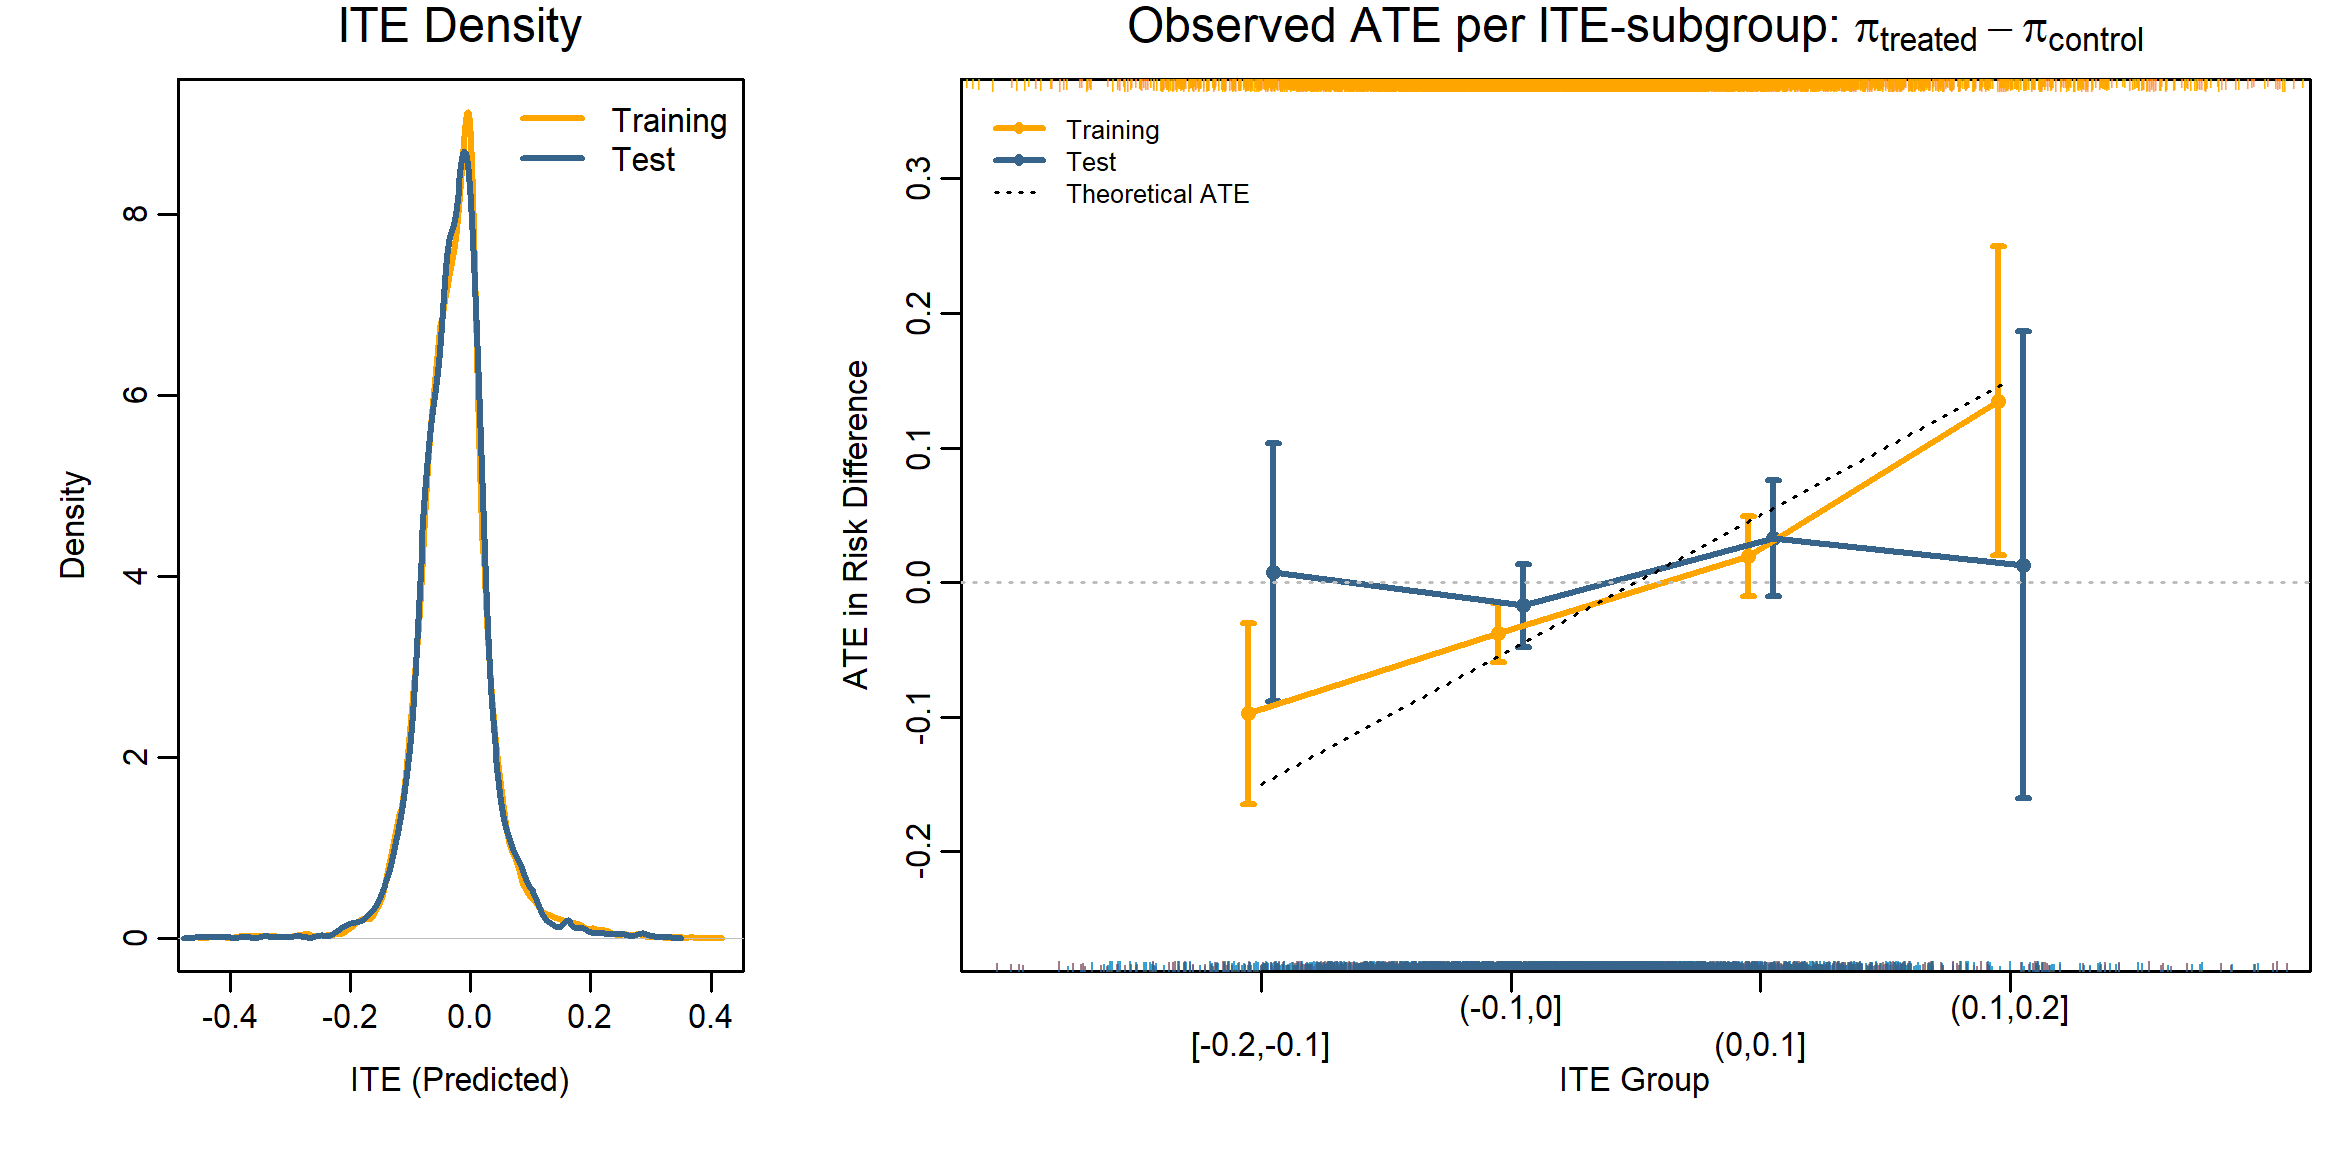
\includegraphics[width=0.9\textwidth]{img/results_IST/glm_tlearner_density_ITE_ATE.png}
\caption{Results for the International Stroke Trial (IST) with the T-learner logistic regression. Left: density of the predicted ITE in the training and test set; Right: observed ATE in terms of risk difference per estimated ITE subgroup.}
\label{fig:IST_density_ITE_ATE_glm_tlearner}
\end{figure}



\begin{figure}[htbp]
\centering
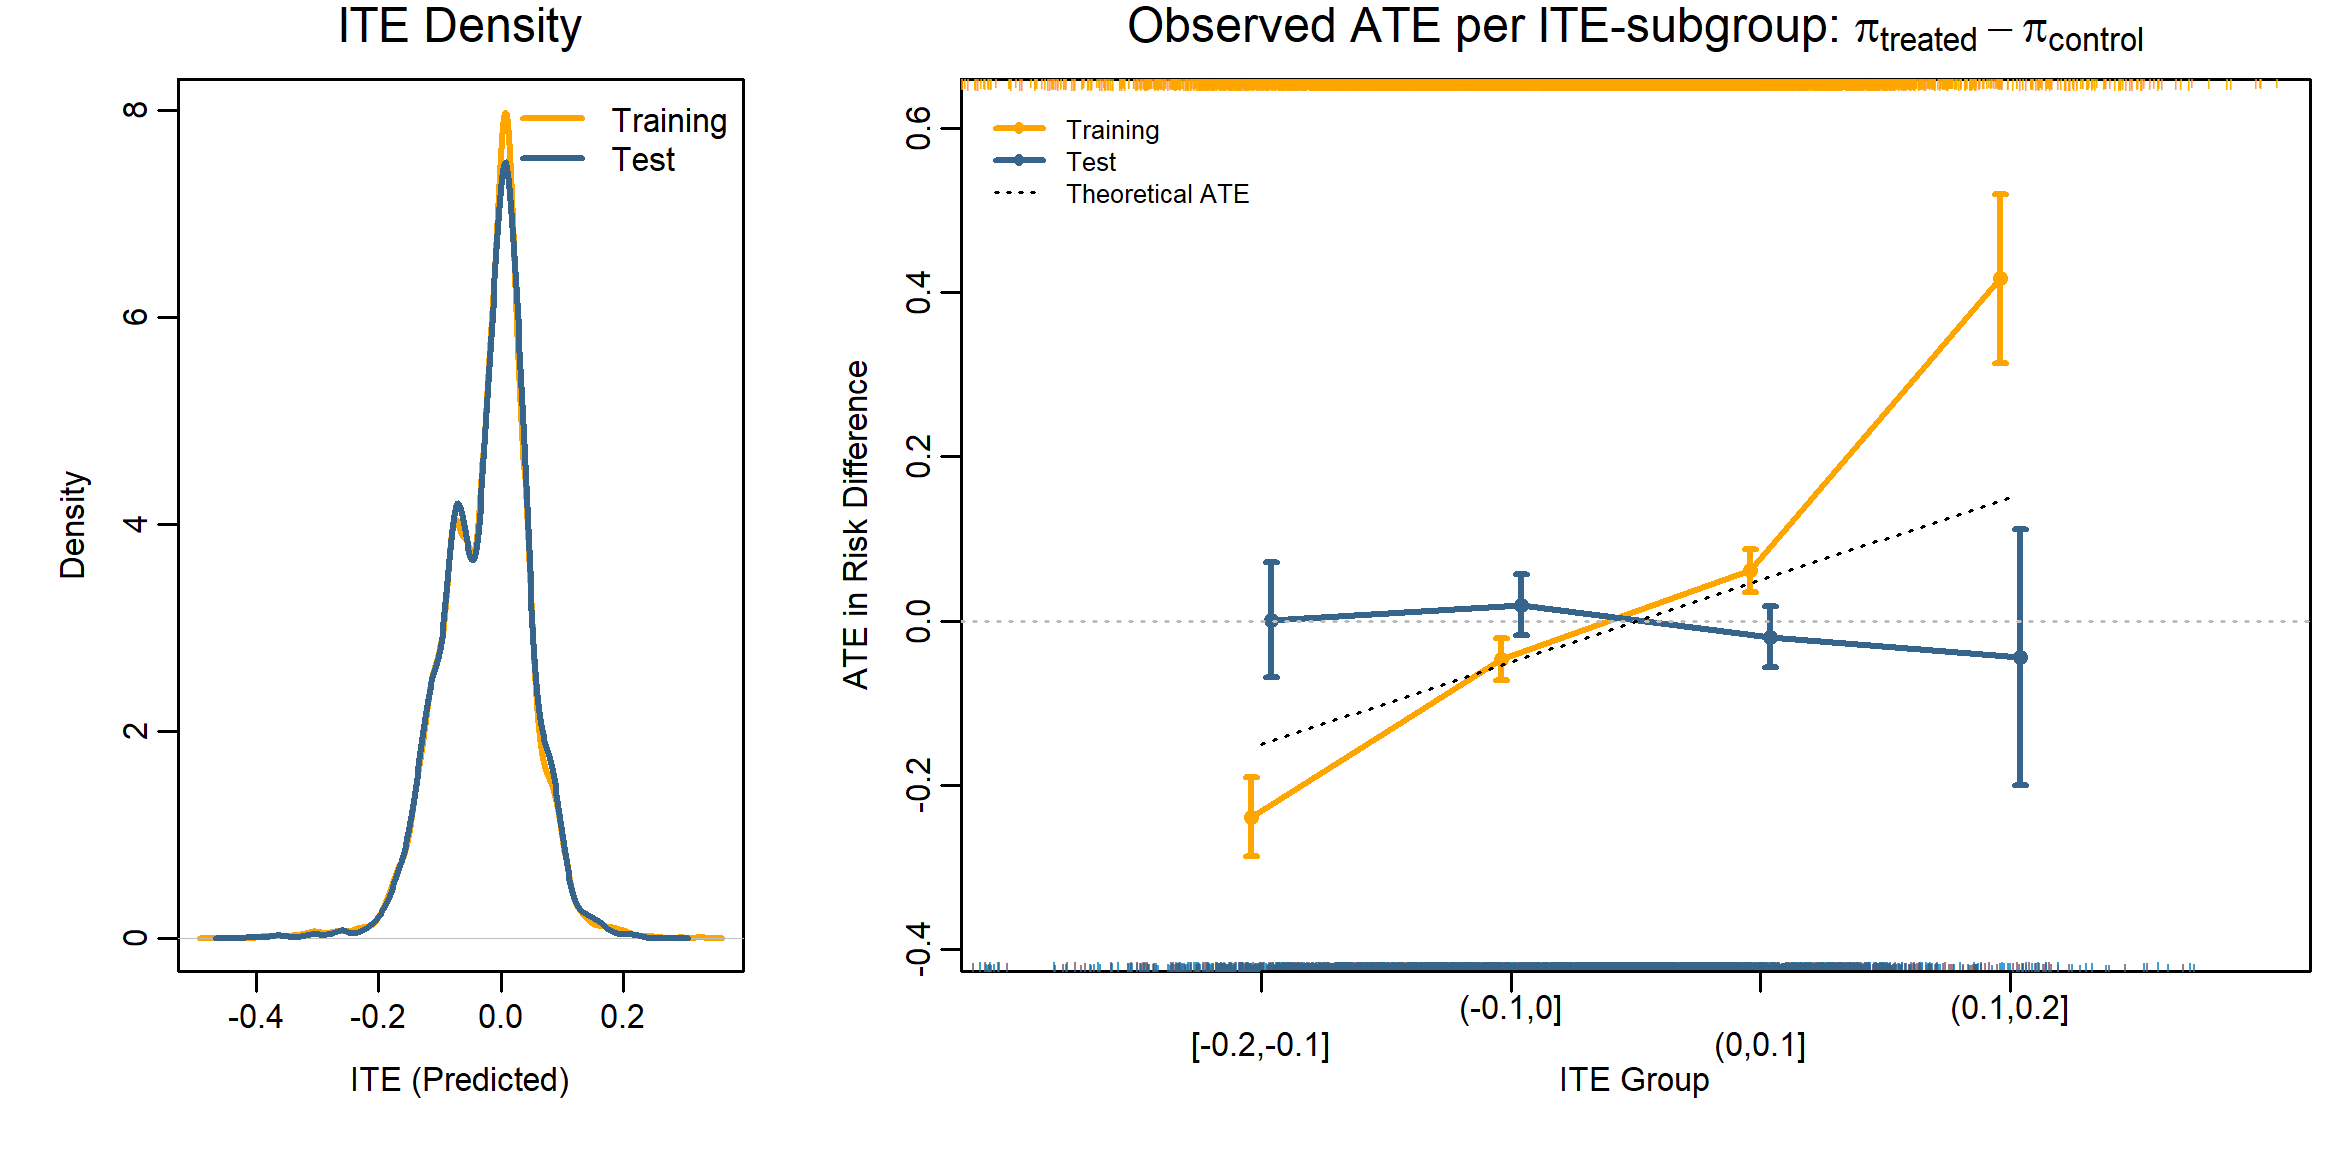
\includegraphics[width=0.9\textwidth]{img/results_IST/IST_tuned_rf_tlearner_density_ITE_ATE.png}
\caption{Results for the International Stroke Trial (IST) with the T-learner tuned random forest. Left: density of the predicted ITE in the training and test set; Right: observed ATE in terms of risk difference per estimated ITE subgroup.}
\label{fig:IST_density_ITE_ATE_tuned_rf}
\end{figure}


\begin{figure}[htbp]
\centering
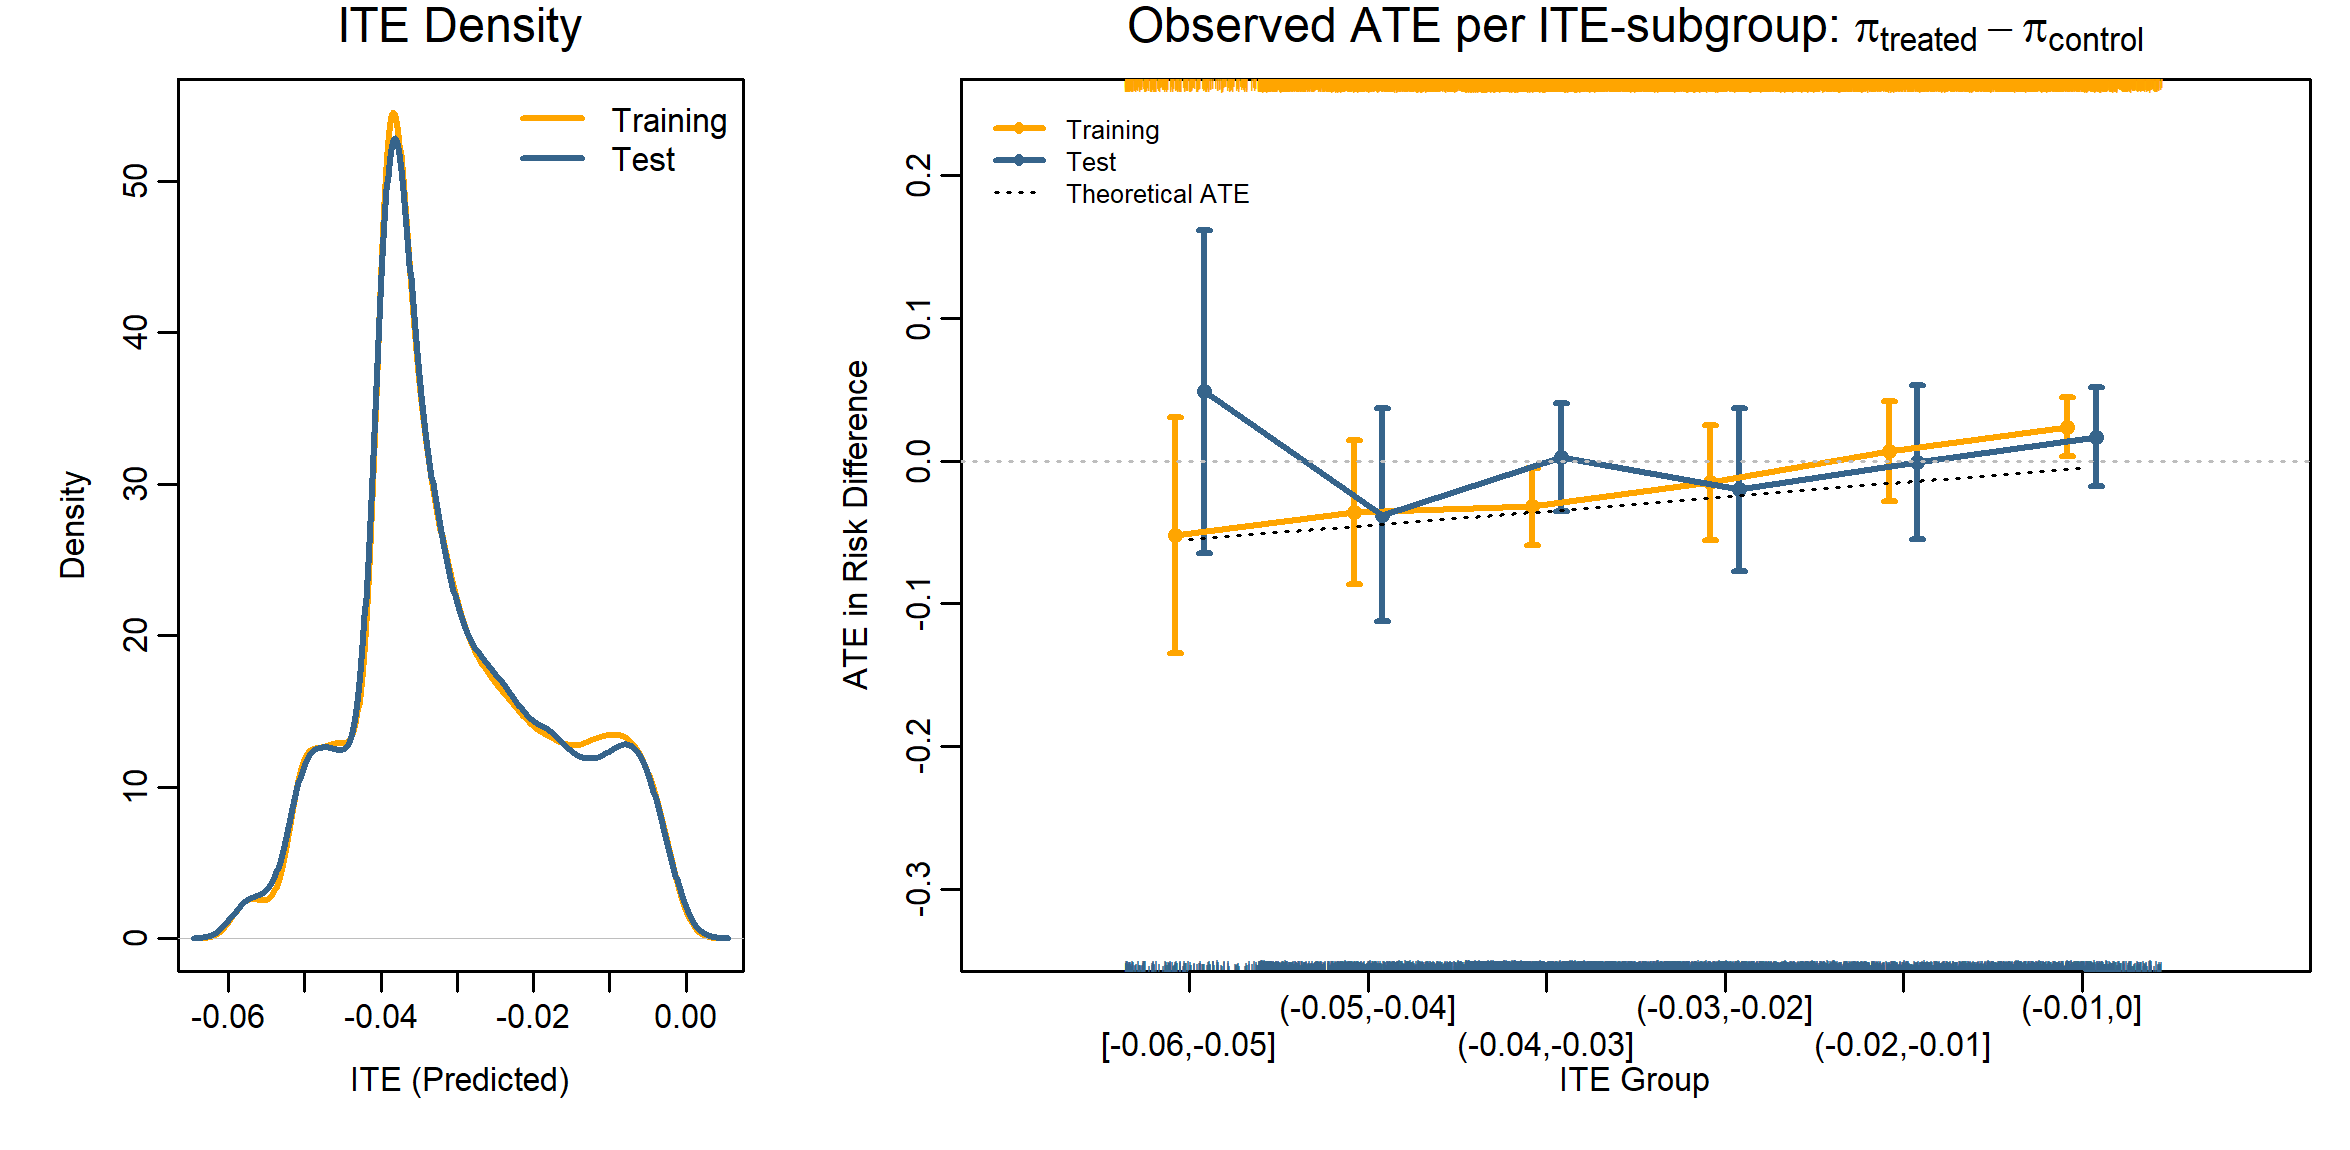
\includegraphics[width=0.9\textwidth]{img/results_IST/IST_TRAM_DAG_slearner_density_ITE_ATE.png}
\caption{Results for the International Stroke Trial (IST) with the S-learner TRAM-DAG. Left: density of the predicted ITE in the training and test set; Right: observed ATE in terms of risk difference per estimated ITE subgroup.}
\label{fig:IST_density_ITE_ATE_TRAM_DAG}
\end{figure}



\clearpage

 
\section{Experiment 3: ITE model robustness under RCT conditions (simulation study)} \label{sec:results_experiment3}

In this section, we present the performance of two causal ML models for estimating the ITE under different scenarios. Scenario 1 represents the ideal case where all variables are observed and treatment effects and heterogeneity are large. Scenario 2 uses the same DGP as in scenario 1 but removes the covariate $X_1$, which has a strong interaction effect with the treatment, from the dataset and treat it as unobserved. Finally, for scenario 3 the coefficients for the direct and interaction treatment effects are weakened, so that heterogeneity is low. All variables are observed again in the last scenario. In each scenario, we applied the T-learner logistic regression and the T-learner tuned random forest. The results of the models on the three scenarios are presented in Figures \ref{fig:fully_observed_glm_tlearner} to \ref{fig:small_interaction_tuned_rf_tlearner}.



\subsection{Scenario (1): Fully observed, large effects}



\begin{figure}[htbp]
\centering
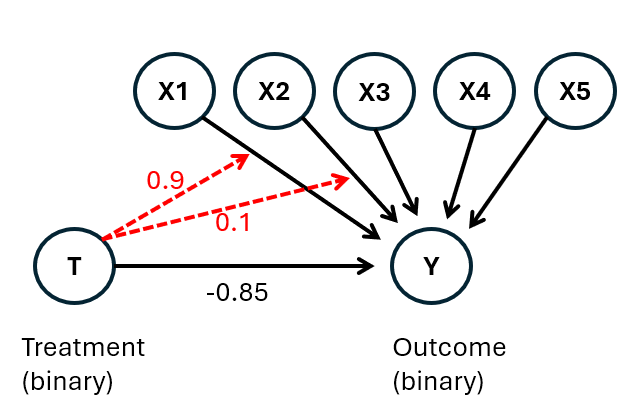
\includegraphics[width=0.35\textwidth]{img/results_ITE_simulation/simulation_observed.png}
\caption{DAG for scenario (1), where all variables are observed and there are strong treatment and interaction effects. The numbers indicate the coefficients on the log-odds-scale. Red: interaction effects between treatment ($T$) and covariates ($X_1$ and $X_2$) on the outcome ($Y$).}
\label{fig:fully_observed_dag}
\end{figure}


\begin{figure}[htbp]
\centering
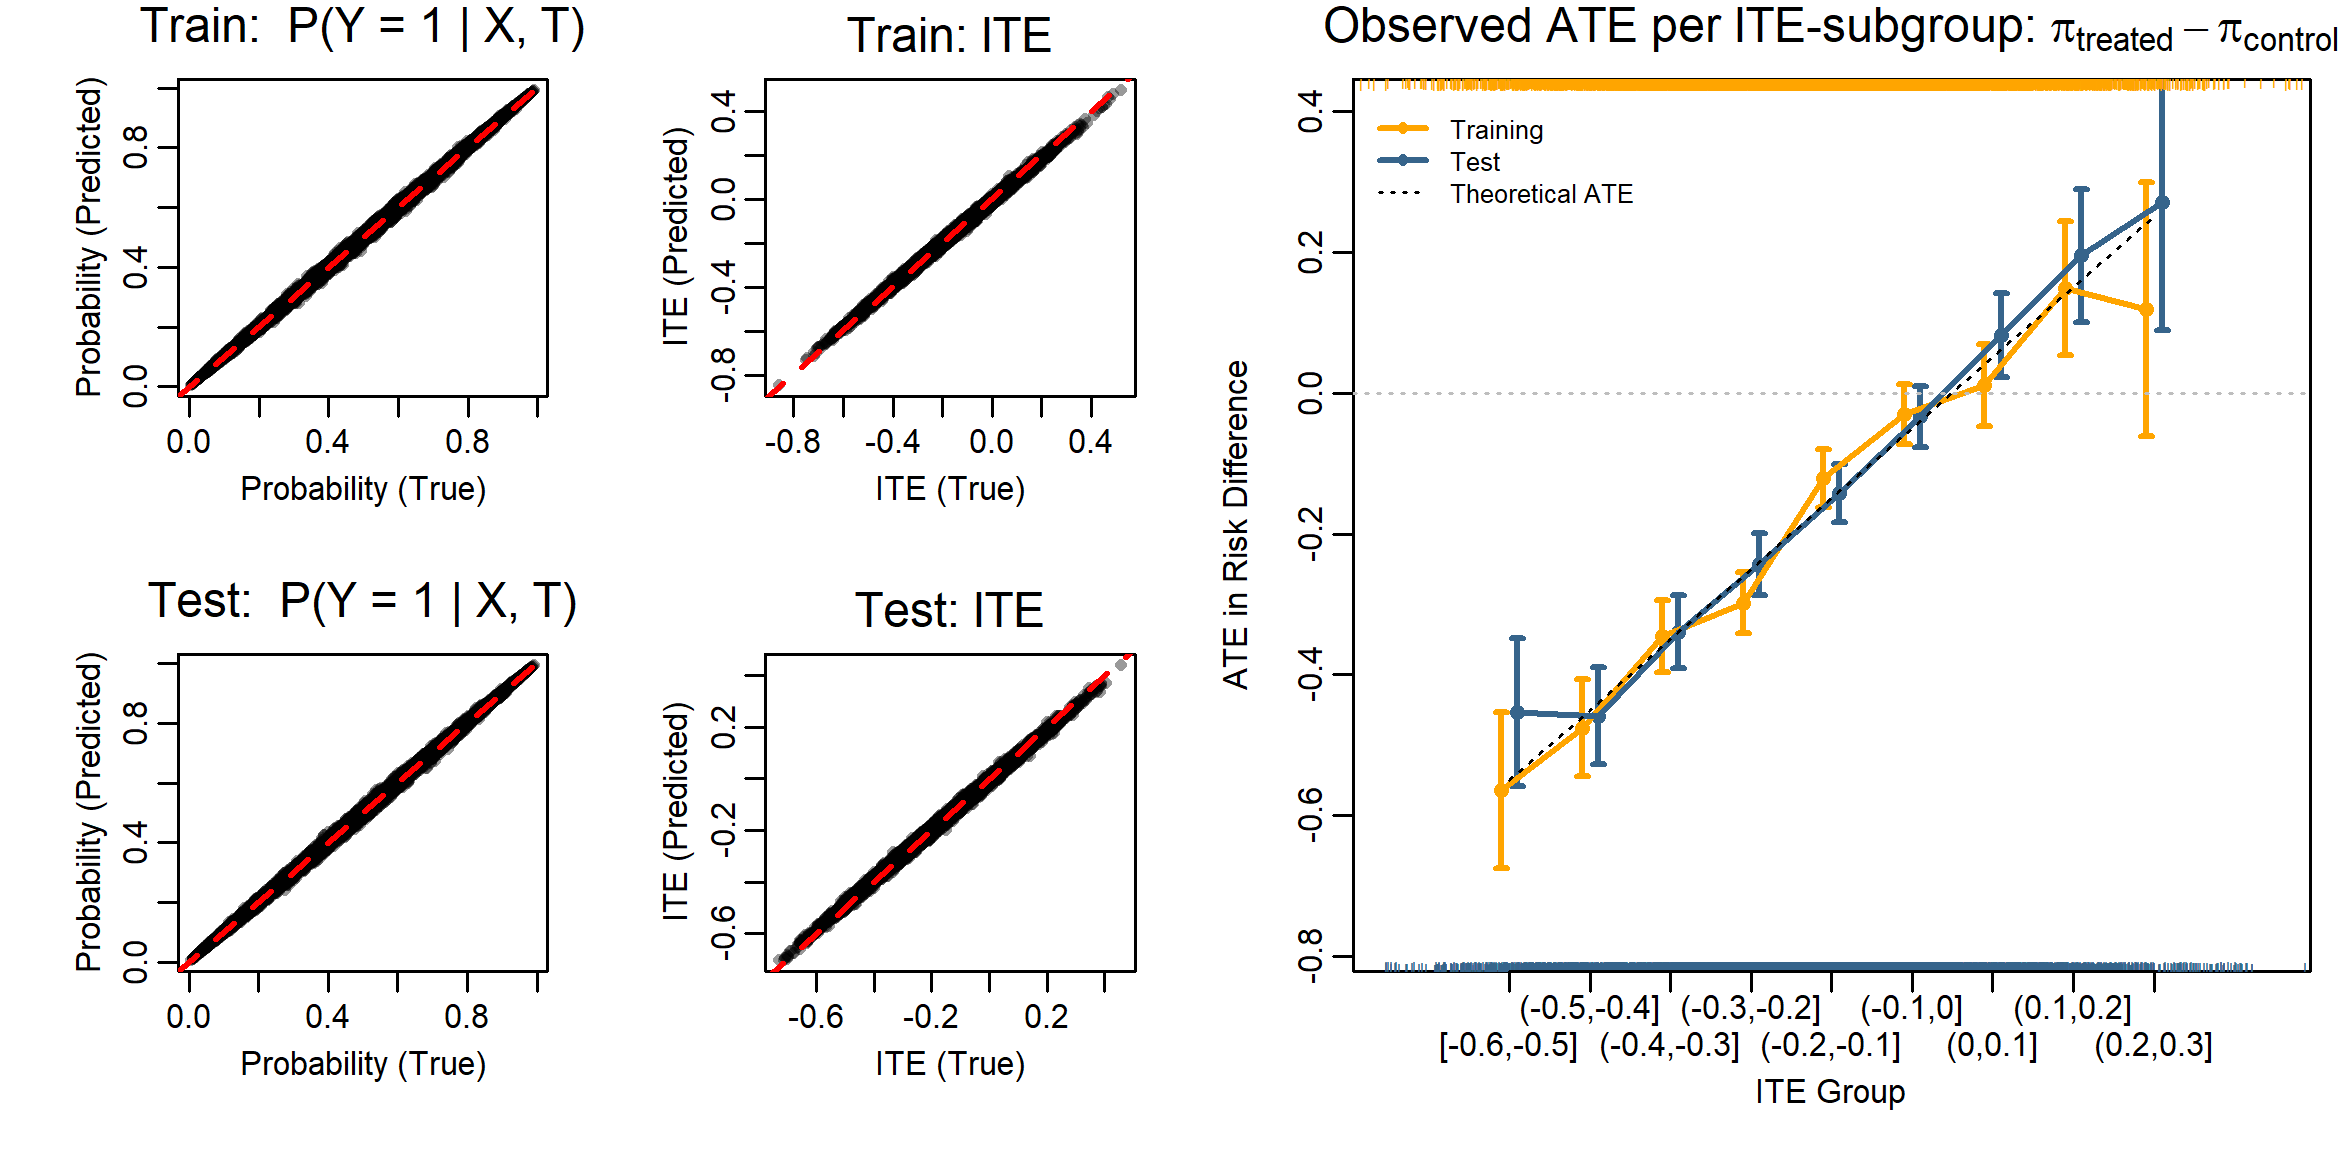
\includegraphics[width=0.9\textwidth]{img/results_ITE_simulation/fully_observed_glm_tlearner.png}
\caption{Results with the T-learner logistic regression in scenario (1) when the DAG is fully observed and there are strong treatment and interaction effects. Left: true vs. predicted probabilities for $\text{P}(Y=1 \mid X, T)$; Middle: true vs. predicted ITEs; Right: observed ATE in terms of risk difference per estimated ITE subgroup.}
\label{fig:fully_observed_glm_tlearner}
\end{figure}


\begin{figure}[htbp]
\centering
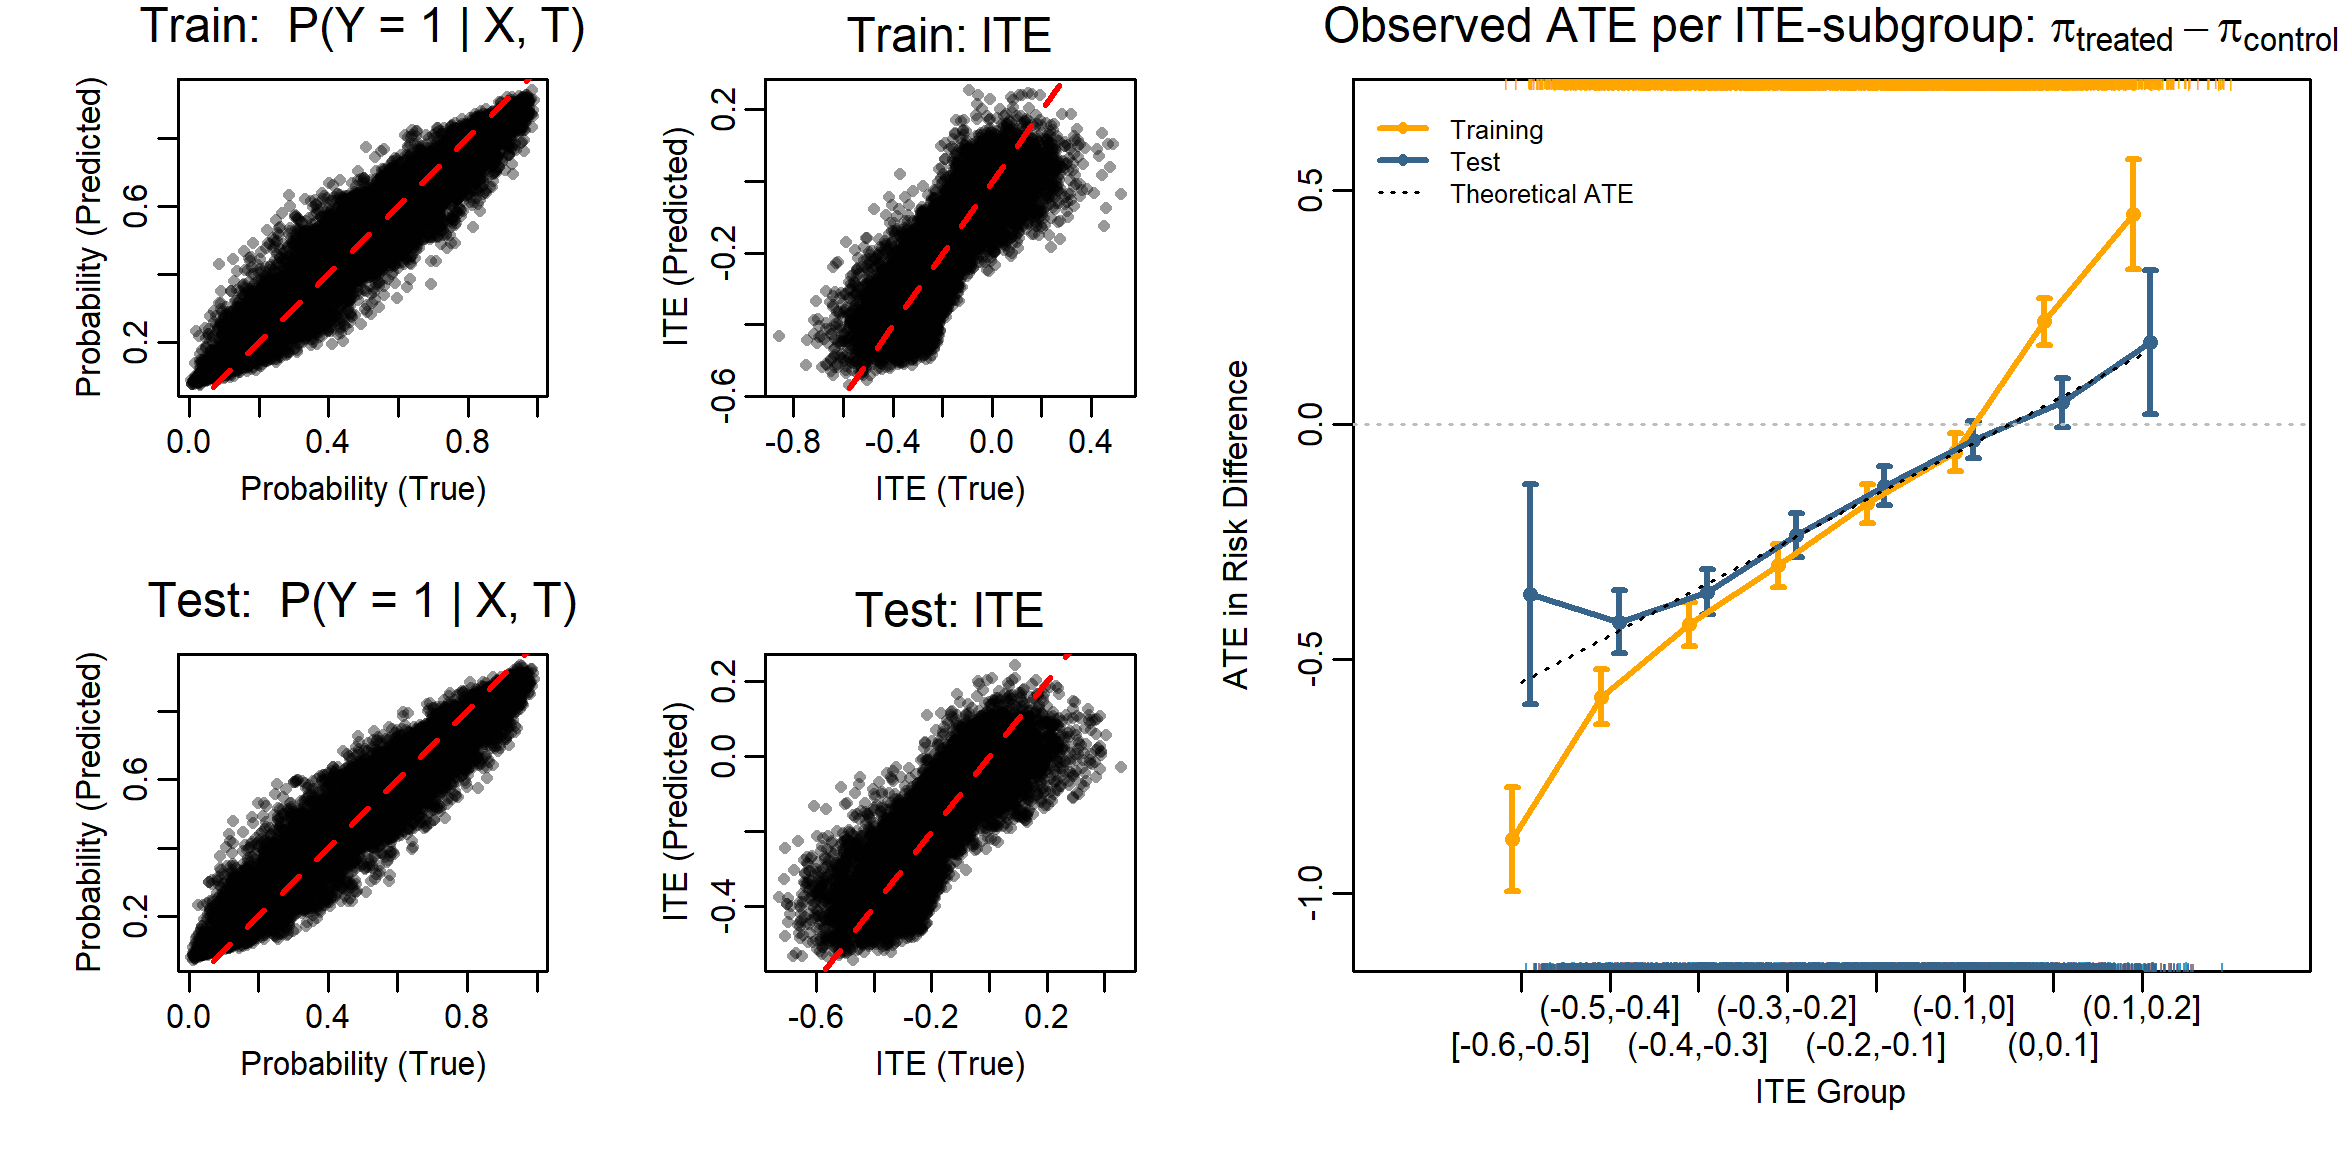
\includegraphics[width=0.9\textwidth]{img/results_ITE_simulation/fully_observed_tuned_rf_tlearner.png}
\caption{Results with the T-learner tuned random forest in scenario (1) when the DAG is fully observed, strong effects. Left: true vs. predicted probabilities for $\text{P}(Y=1 \mid X, T)$; Middle: true vs. predicted ITEs; Right: observed ATE in terms of risk difference per estimated ITE subgroup.}
\label{fig:fully_tuned_rf_tlearner}
\end{figure}


\clearpage



\subsection{Scenario (2): unobserved interaction}

\begin{figure}[htbp]
\centering
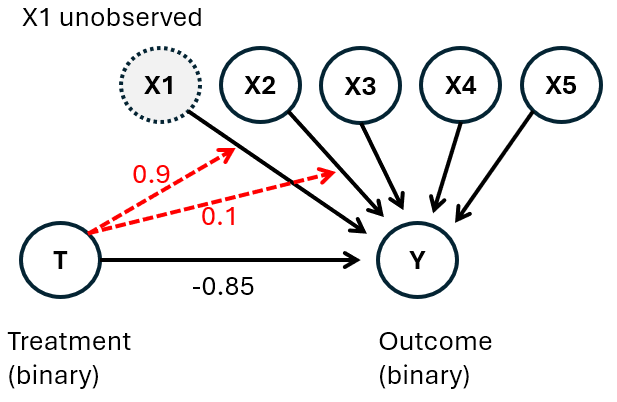
\includegraphics[width=0.35\textwidth]{img/results_ITE_simulation/simulation_unobserved.png}
\caption{DAG for scenario (2), where there are strong treatment and interaction effects, but variable $X1$ is not observed. The numbers indicate the coefficients on the log-odds-scale. Red: interaction effects between treatment ($T$) and covariates ($X_1$ and $X_2$) on the outcome ($Y$).}
\label{fig:unobserved_interaction_dag}
\end{figure}



\begin{figure}[htbp]
\centering
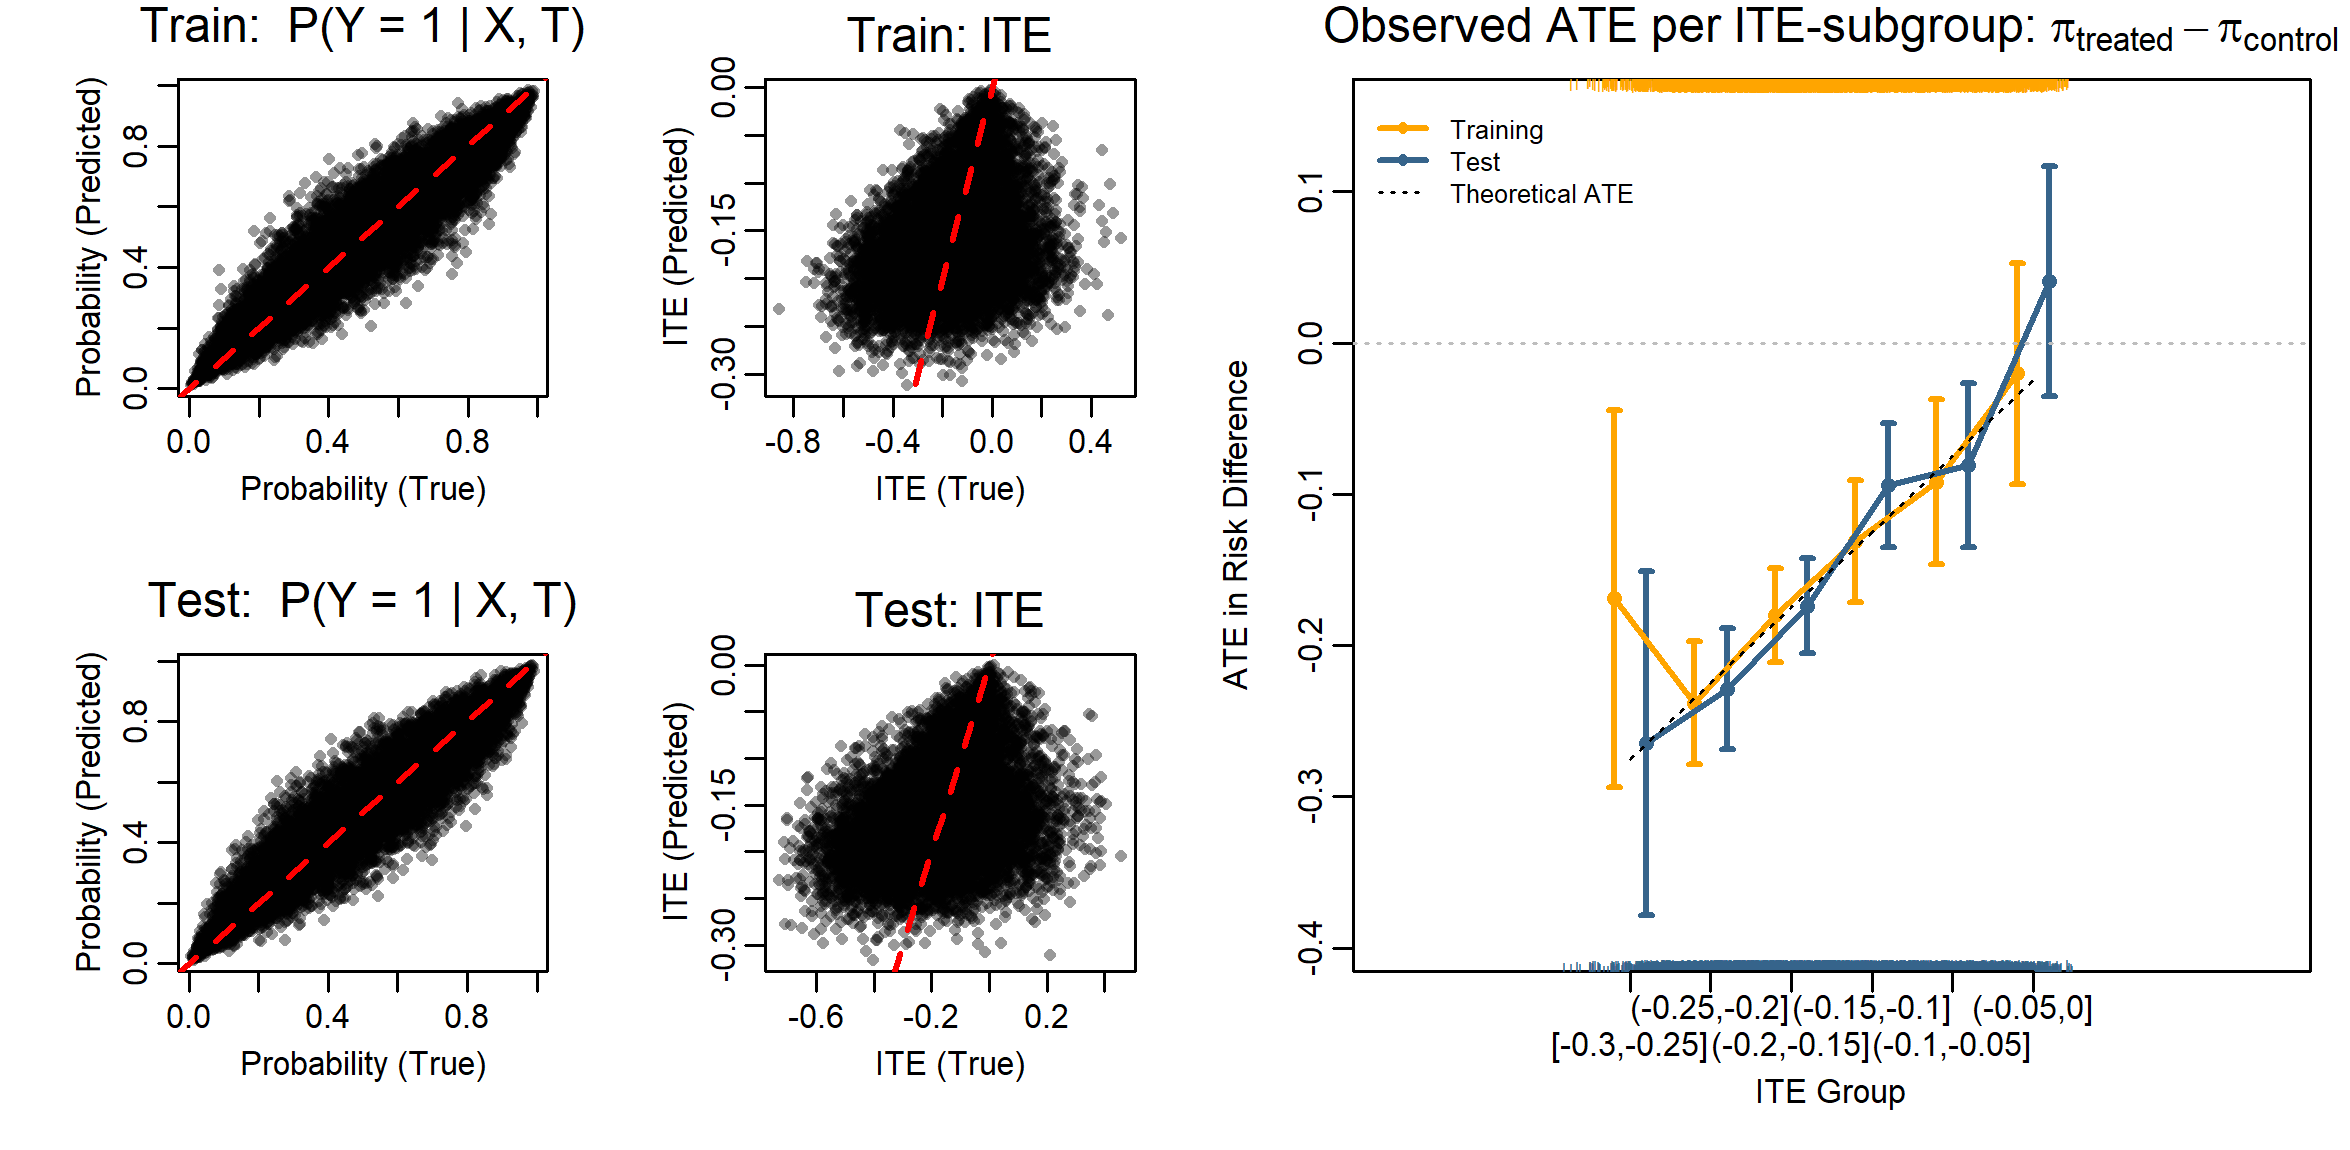
\includegraphics[width=0.9\textwidth]{img/results_ITE_simulation/unobserved_interaction_glm_tlearner.png}
\caption{Results with the T-learner logistic regression in scenario (2) when there are strong treatment and interaction effects, but variable $X_1$ is not observed. Left: true vs. predicted probabilities for $\text{P}(Y=1 \mid X, T)$; Middle: true vs. predicted ITEs; Right: observed ATE in terms of risk difference per estimated ITE subgroup.}
\label{fig:unobserved_interaction_glm_tlearner}
\end{figure}



\begin{figure}[htbp]
\centering
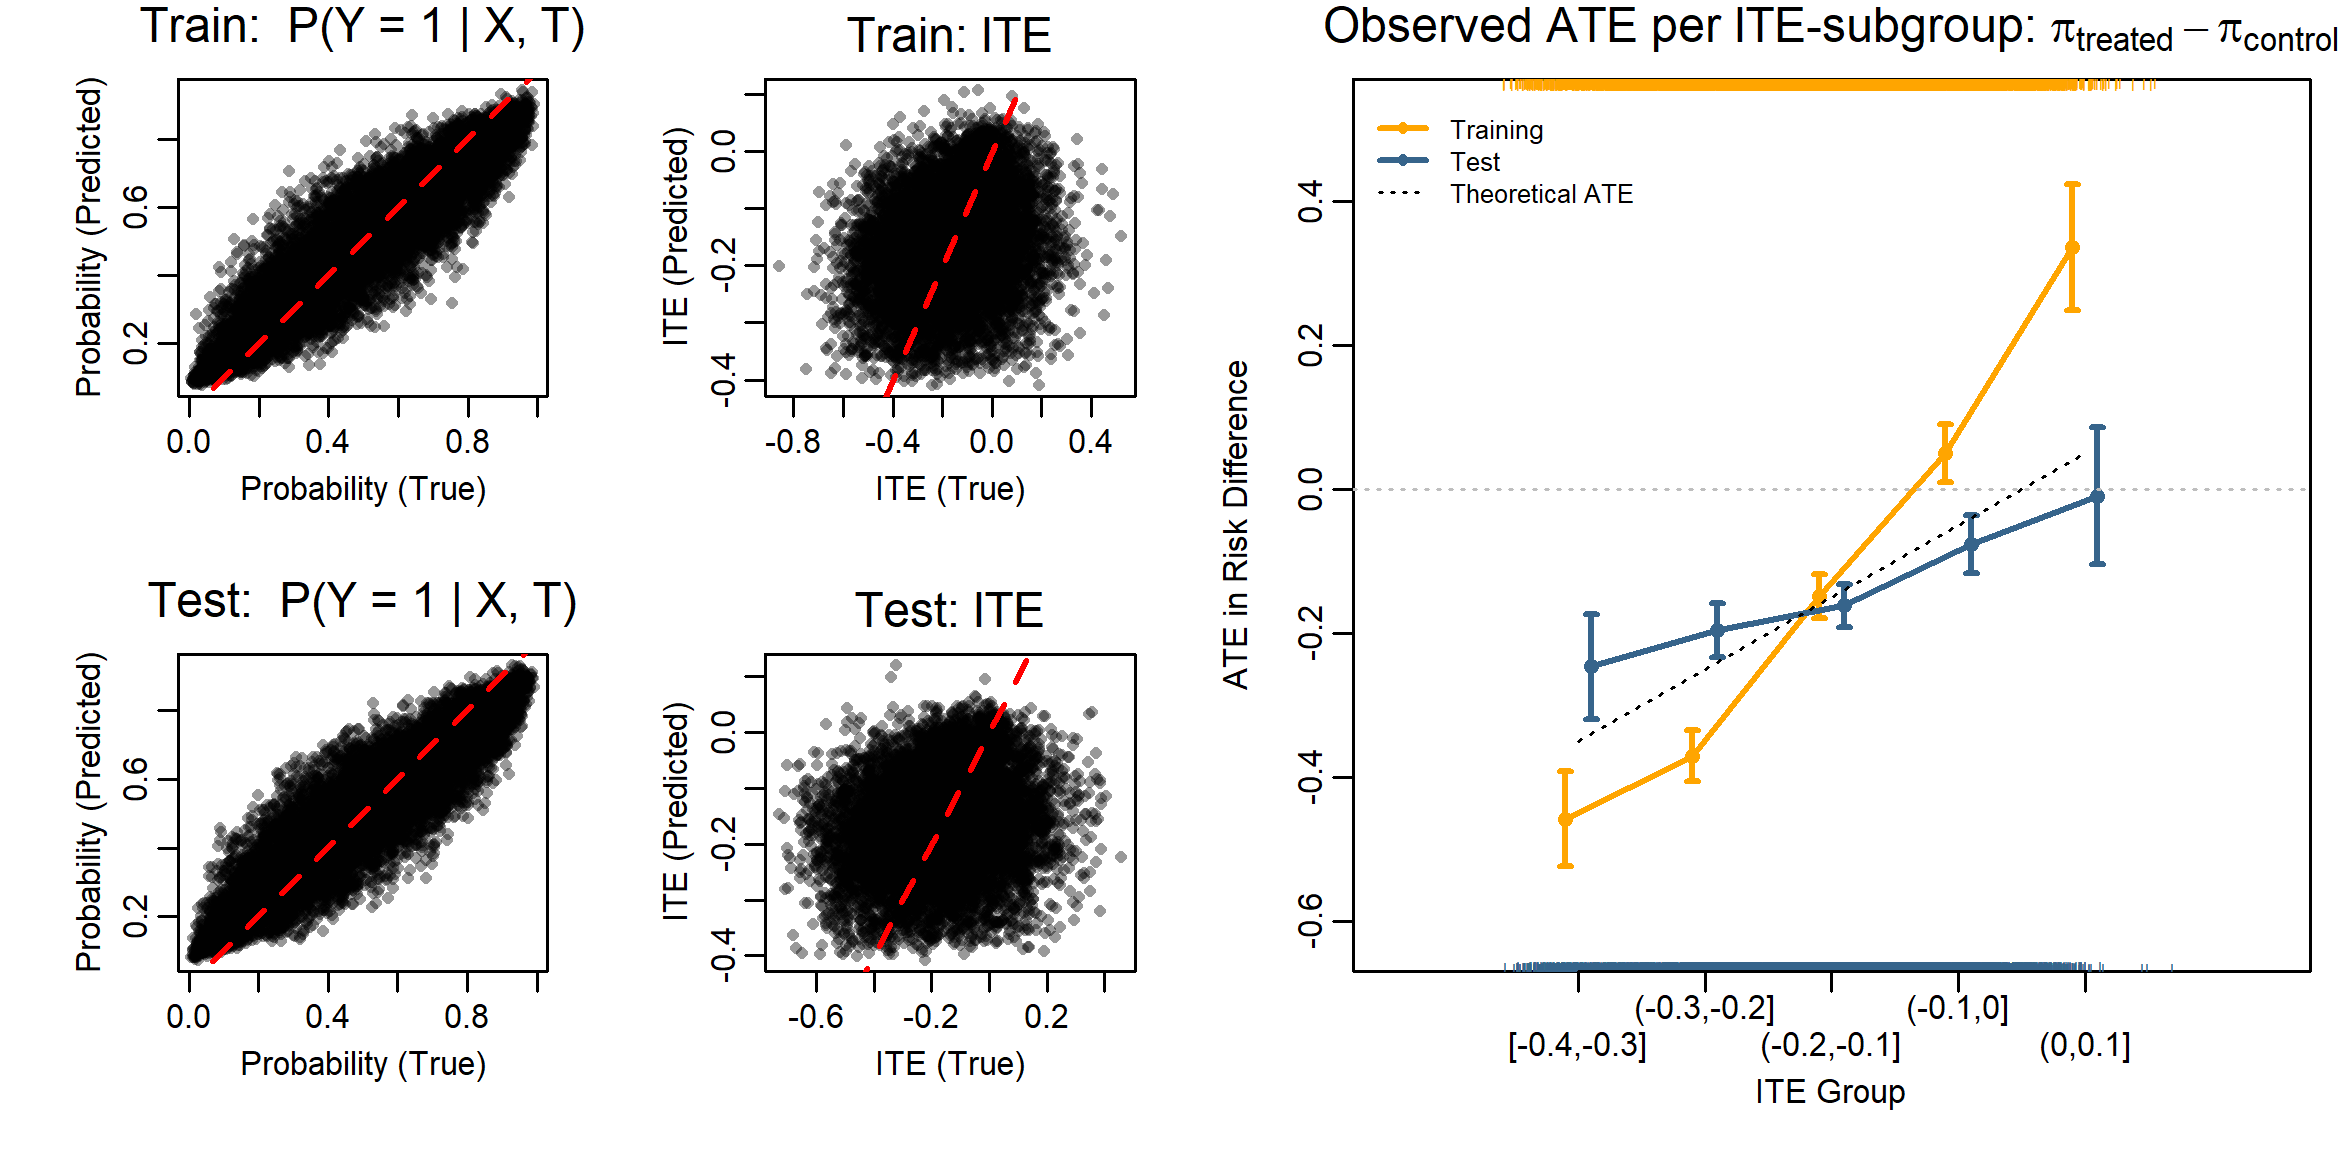
\includegraphics[width=0.9\textwidth]{img/results_ITE_simulation/unobserved_interaction_tuned_rf_tlearner.png}
\caption{Results with the T-learner tuned random forest in scenario (2) when there are strong treatment and interaction effects, but variable $X_1$ is not observed. Left: true vs. predicted probabilities for $\text{P}(Y=1 \mid X, T)$; Middle: true vs. predicted ITEs; Right: observed ATE in terms of risk difference per estimated ITE subgroup.}
\label{fig:unobserved_interaction_tuned_rf_tlearner}
\end{figure}


\clearpage

\subsection{Scenario (3): Fully observed, small effects}

\begin{figure}[htbp]
\centering
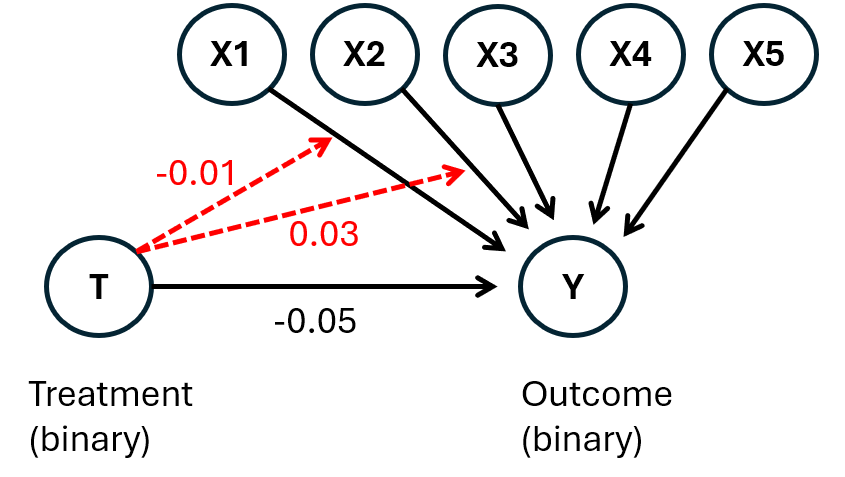
\includegraphics[width=0.35\textwidth]{img/results_ITE_simulation/simulation_small_effects.png}
\caption{DAG for scenario (3), where all variables are observed and there are weak treatment and interaction effects. The numbers indicate the coefficients on the log-odds-scale. Red: interaction effects between treatment ($T$) and covariates ($X_1$ and $X_2$) on the outcome ($Y$).}
\label{fig:small_interaction_dag}
\end{figure}




\begin{figure}[htbp]
\centering
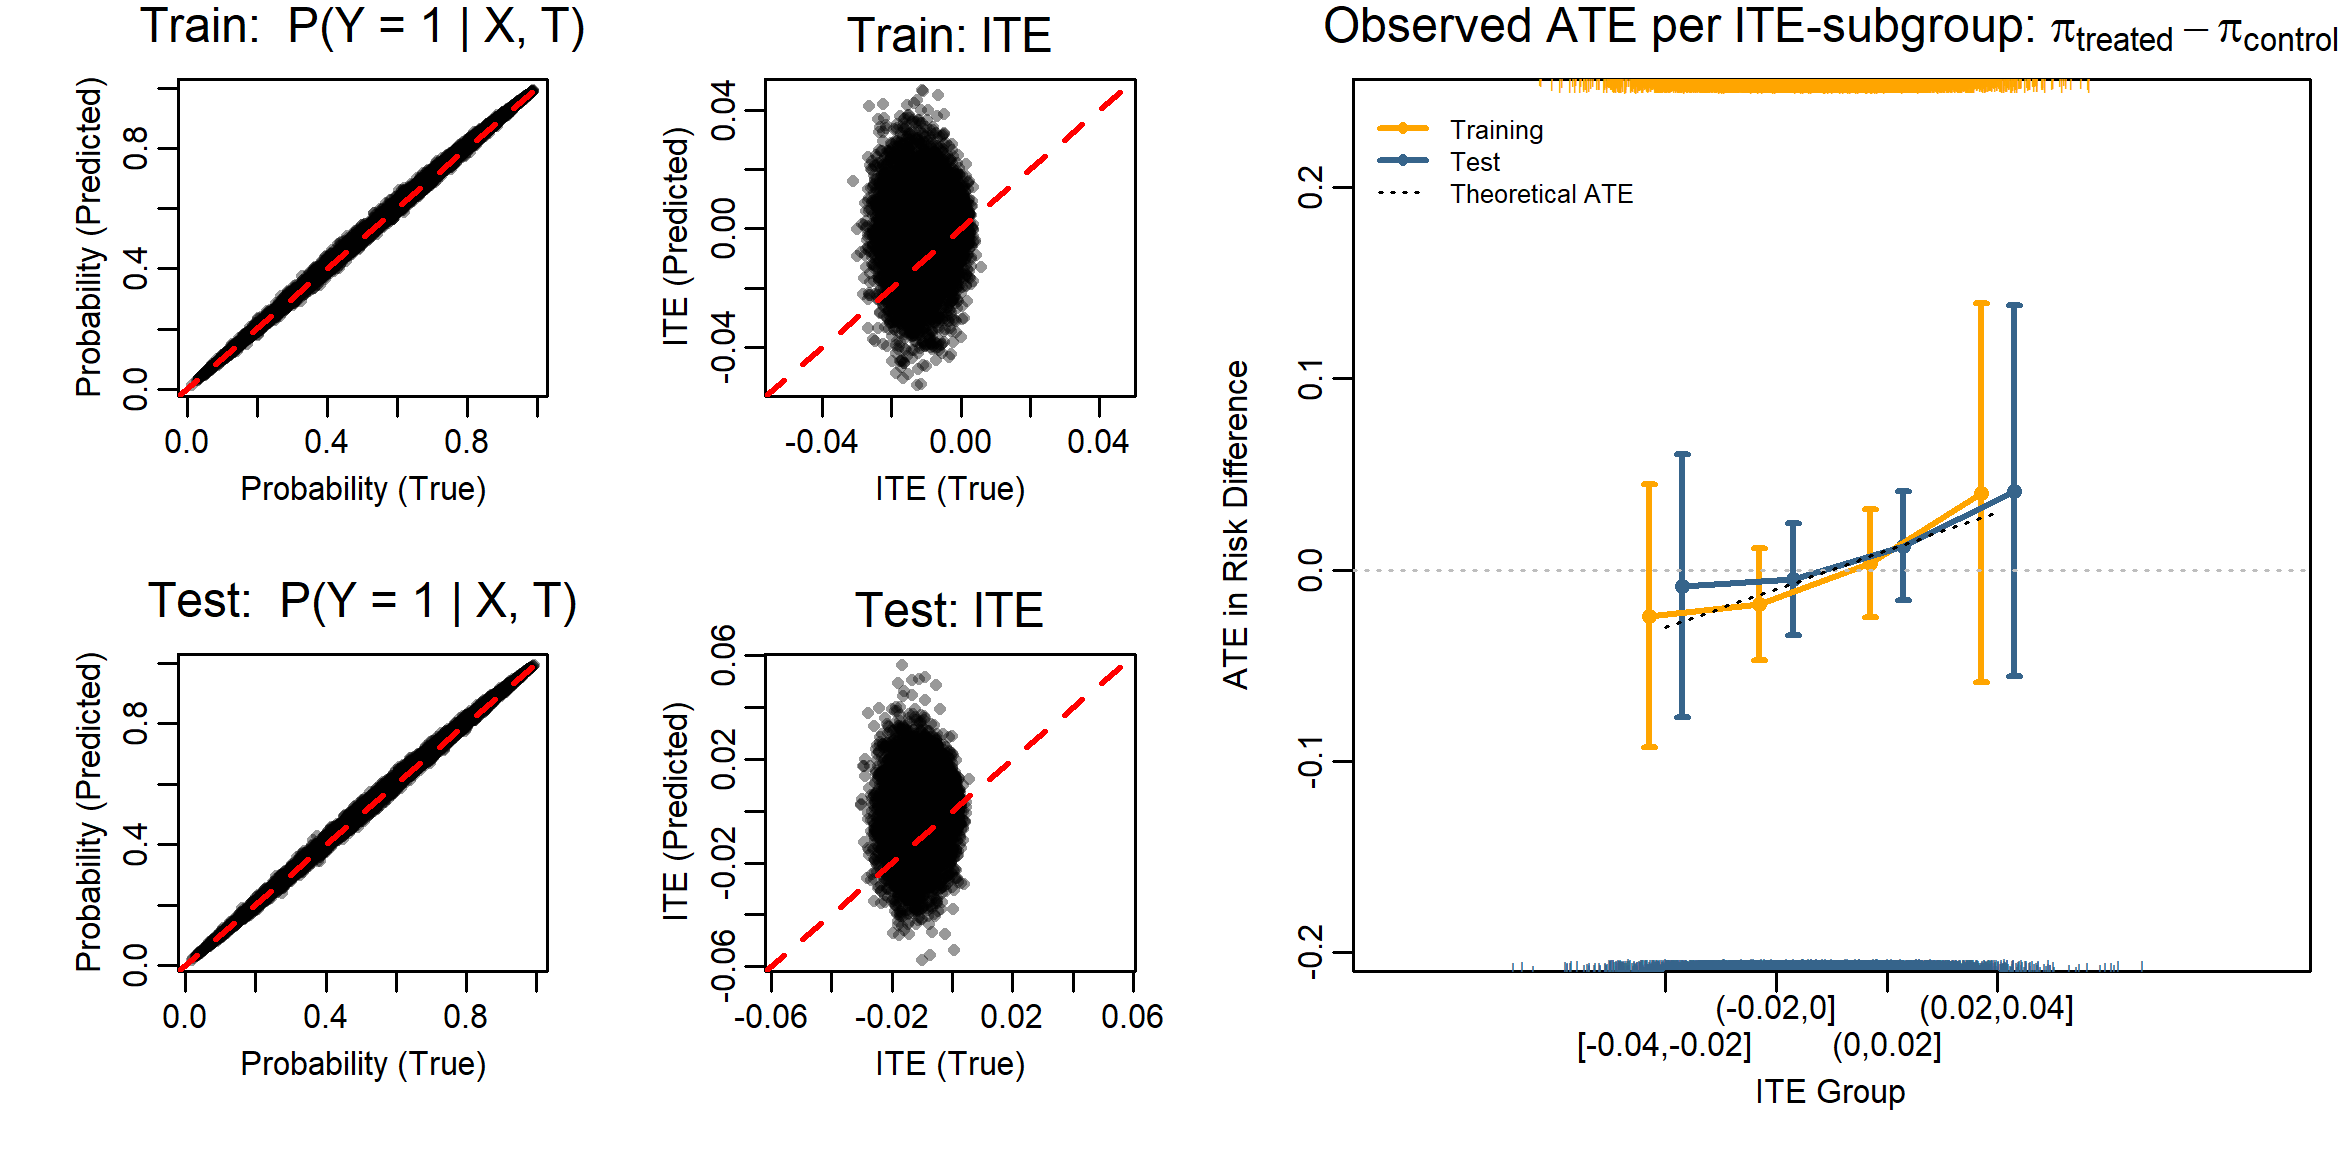
\includegraphics[width=0.9\textwidth]{img/results_ITE_simulation/small_interaction_glm_tlearner.png}
\caption{Results with the T-learner logistic regression in scenario (3) when the DAG is fully observed and there are weak treatment and interaction effects. Left: true vs. predicted probabilities for $\text{P}(Y=1 \mid X, T)$; Middle: true vs. predicted ITEs; Right: observed ATE in terms of risk difference per estimated ITE subgroup.}
\label{fig:small_interaction_glm_tlearner}
\end{figure}




\begin{figure}[htbp]
\centering
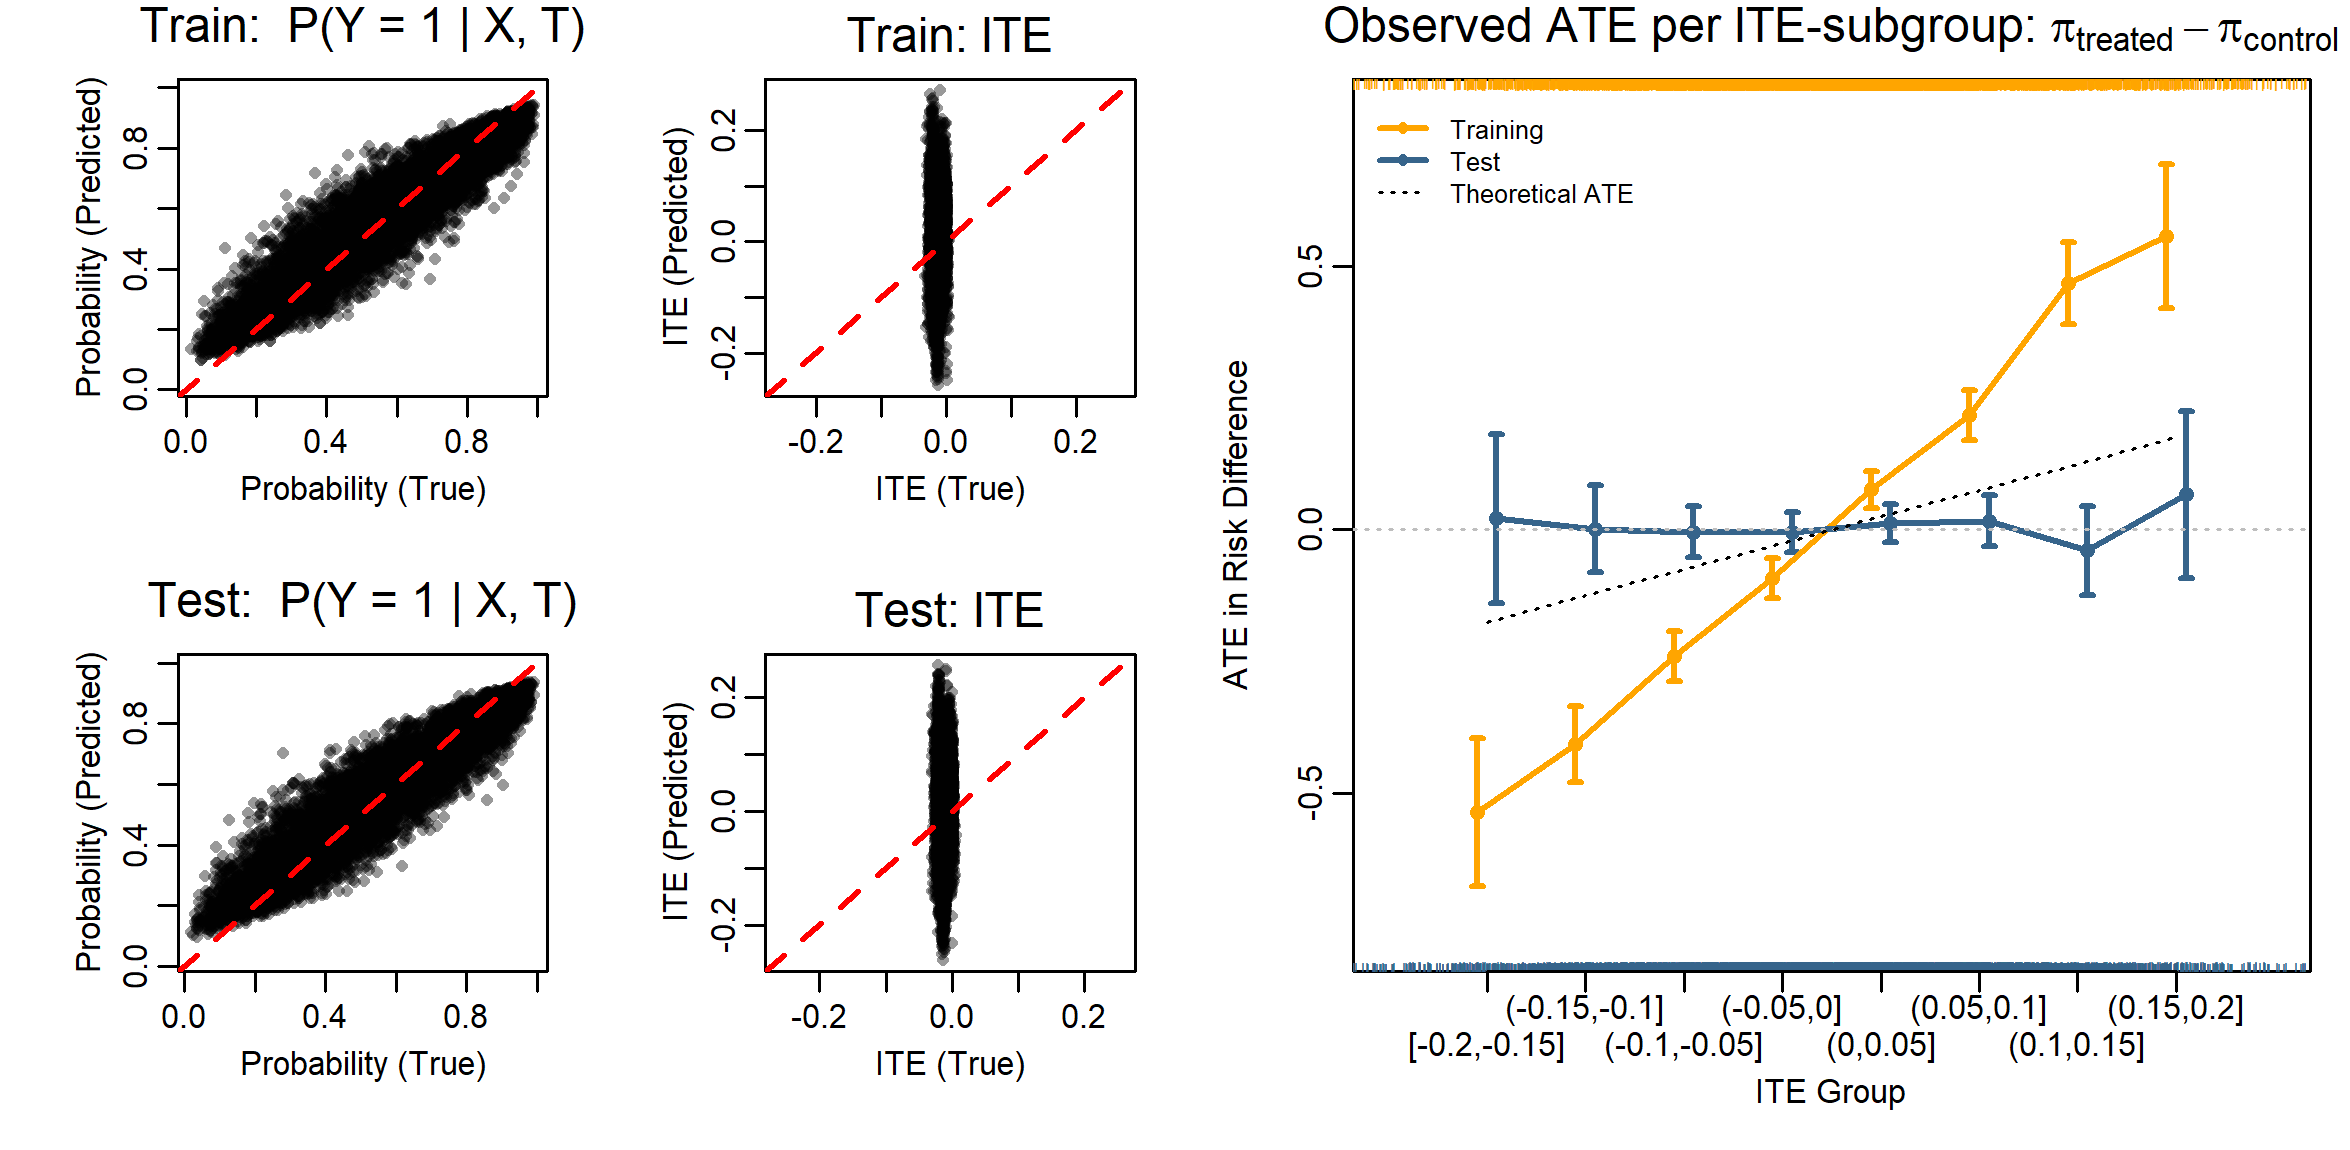
\includegraphics[width=0.9\textwidth]{img/results_ITE_simulation/small_interaction_tuned_rf_tlearner.png}
\caption{Results with the T-learner tuned random forest in scenario (3) when the DAG is fully observed and there are weak treatment and interaction effects. Left: true vs. predicted probabilities for $\text{P}(Y=1 \mid X, T)$; Middle: true vs. predicted ITEs; Right: observed ATE in terms of risk difference per estimated ITE subgroup.}
\label{fig:small_interaction_tuned_rf_tlearner}
\end{figure}


\clearpage


\section{ITE estimation with TRAM-DAGs (simulation study)}

First, we present the results for scenario (1) with a direct and interaction effect. Then, we present the results for scenario (2) with a direct effect but no interaction effects, and finally, scenario (3) with interaction effects but no direct effect of the treatment. For each scenario, we compare the results in an observational setting with confounded treatment allocation and in a randomized controlled trial (RCT) setting without confounders. We also compare the average treatment effect (ATE), which can directly be calculated in the RCT, with the ATE based on the estimated individualized treatment effects. If the estimated ITEs are unbiased, they should be a good estimate of the ATE. All ITEs presented in this section are technically quantile treatment effects (QTEs) based on the 0.5-quantile of the potential outcomes. For simplicity we will refer to them as ITEs in the following.


\subsection{Scenario (1): Direct and interaction effects} 

Scenario (1) included a direct effect of the treatment on the outcome and an additional interaction effect of the treatment with the covariates X2 and X3. A train and test set were generated with 20'000 observations each. In the observational setting, the treatment allocation was confounded by the covariates X1 and X2.  In the train set, $38.6$\% of patients were in the control group and $61.4$\% were in the treatment group. This ratio was similar in the test set. In the RCT setting treatment allocation was randomized. In the train set $49.8$\% individuals were in the control group and $50.2$\% in the treatment group. In the test set $50.2$\% were in the control group and $49.8$\% in the treatment group. Figure \ref{fig:scenario1_ite_distribution_dgp} illustrates the true ITE distribution that resulted from the DGP. Due to the interaction effects, there is some heterogeneity in the ITE distribution. Figure \ref{fig:scenario1_sampling_distributions_vertical} shows the marginal distributions of all variables according to the DGP and the estimates of the fitted TRAM-DAG. Figure \ref{fig:scenario1_outcome_distributions} shows the distribution of the outcome under the do(Tr=0) and do(Tr=1) interventions. The fitted model was applied to estimate the ITEs in terms of the difference in medians of the potential outcomes. The resulting density of the estimated ITEs compared to the true ITEs according to the DGP is shown in Figure \ref{fig:scenario1_ite_densities_train_test}. Across both settings, the densities of the estimated ITEs are close to the true densities in both the training and test datasets. Figure \ref{fig:scenario1_ite_scatter_train_test} shows the scatterplots of true against estimated ITEs. Finally, Figure \ref{fig:scenario1_ite_cATE} displays the ITE-ATE plot where the ATE is computed as the difference in medians of the observed outcome under the treatments within the respective ITE-subgroups The trends observed in the training and test sets are consistent.

The average treatment effect (ATE) is presented in Table \ref{tab:scenario1_ate_comparison}. In the RCT setting in the training set, the difference in means of the outcomes in the two treatment groups was $-0.563$ with a confidence interval of $-0.582$ to $-0.543$. The ATE in terms of the difference in medians of the observed outcomes was $-0.626$. Also in the training set, the ATE in terms of the mean of the true ITEs was $-0.62$ and the ATE in terms of the mean of the estimated ITEs was $-0.619$. All measures, including the ones from the test datasets, are shown in Table \ref{tab:scenario1_ate_comparison}.

NOTE: also add CIs in the table with the ATEs?

\begin{table}[htbp]
\centering
\small
\caption{Scenario (1), including direct and interaction effects: Comparison of ATE measures across train and test sets for the observational and RCT setting.}
\label{tab:scenario1_ate_comparison}
\begin{tabular}{l c c c c}
\toprule
\textbf{Measure} & \multicolumn{2}{c}{\textbf{Observational}} & \multicolumn{2}{c}{\textbf{RCT}} \\
\cmidrule(lr){2-3} \cmidrule(lr){4-5}
 & \textbf{Train} & \textbf{Test} & \textbf{Train} & \textbf{Test} \\
\midrule
ATE as $\text{mean}(\text{Y}_\text{observed}^{(1)}) - \text{mean}(\text{Y}_\text{observed}^{(0)})$ & NA & NA & -0.563 & -0.563 \\
ATE as $\text{median}(\text{Y}_\text{observed}^{(1)}) - \text{median}(\text{Y}_\text{observed}^{(0)})$  & NA & NA & -0.626 & -0.638 \\
ATE as mean(ITE$_\text{true}$)  & -0.62 & -0.622 & -0.62 & -0.622 \\
ATE as mean(ITE$_\text{estimated}$) & -0.617 & -0.62 & -0.619 & -0.622 \\
\bottomrule
\end{tabular}
\end{table}




\begin{figure}[htbp]
\centering
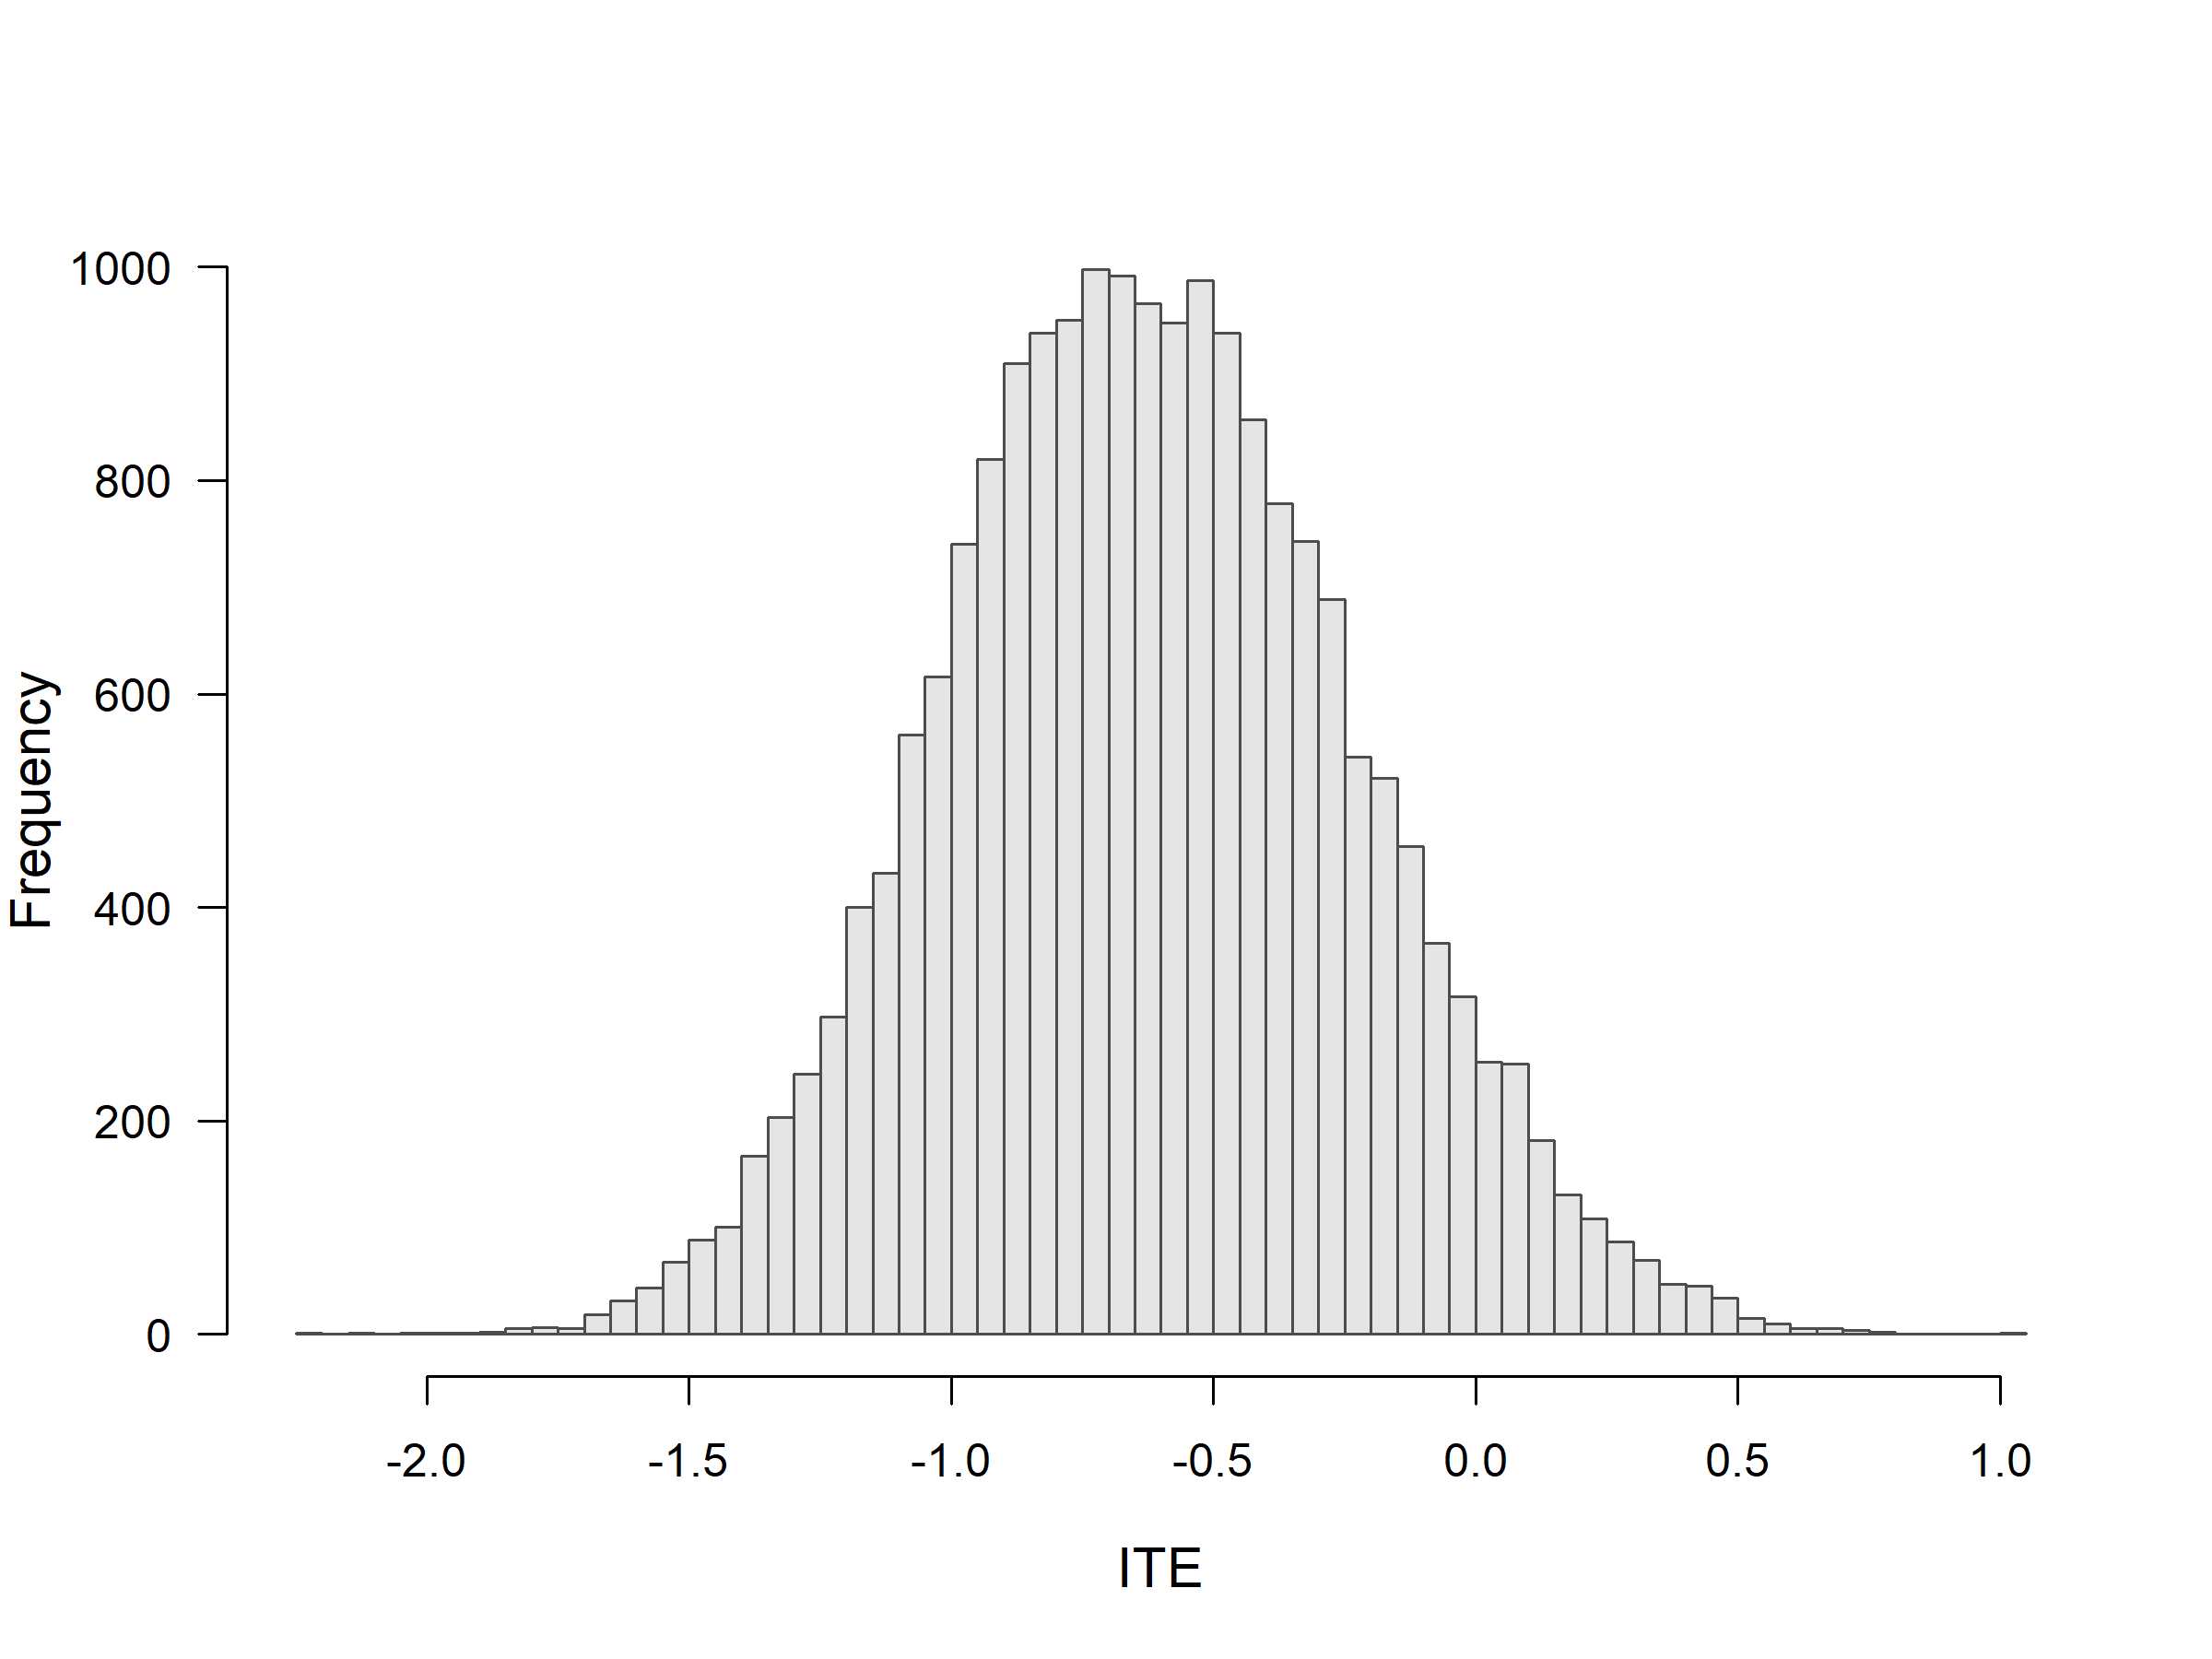
\includegraphics[width=0.45\textwidth]{img/results/observ_scenario1_ite_distribution_dgp.png}
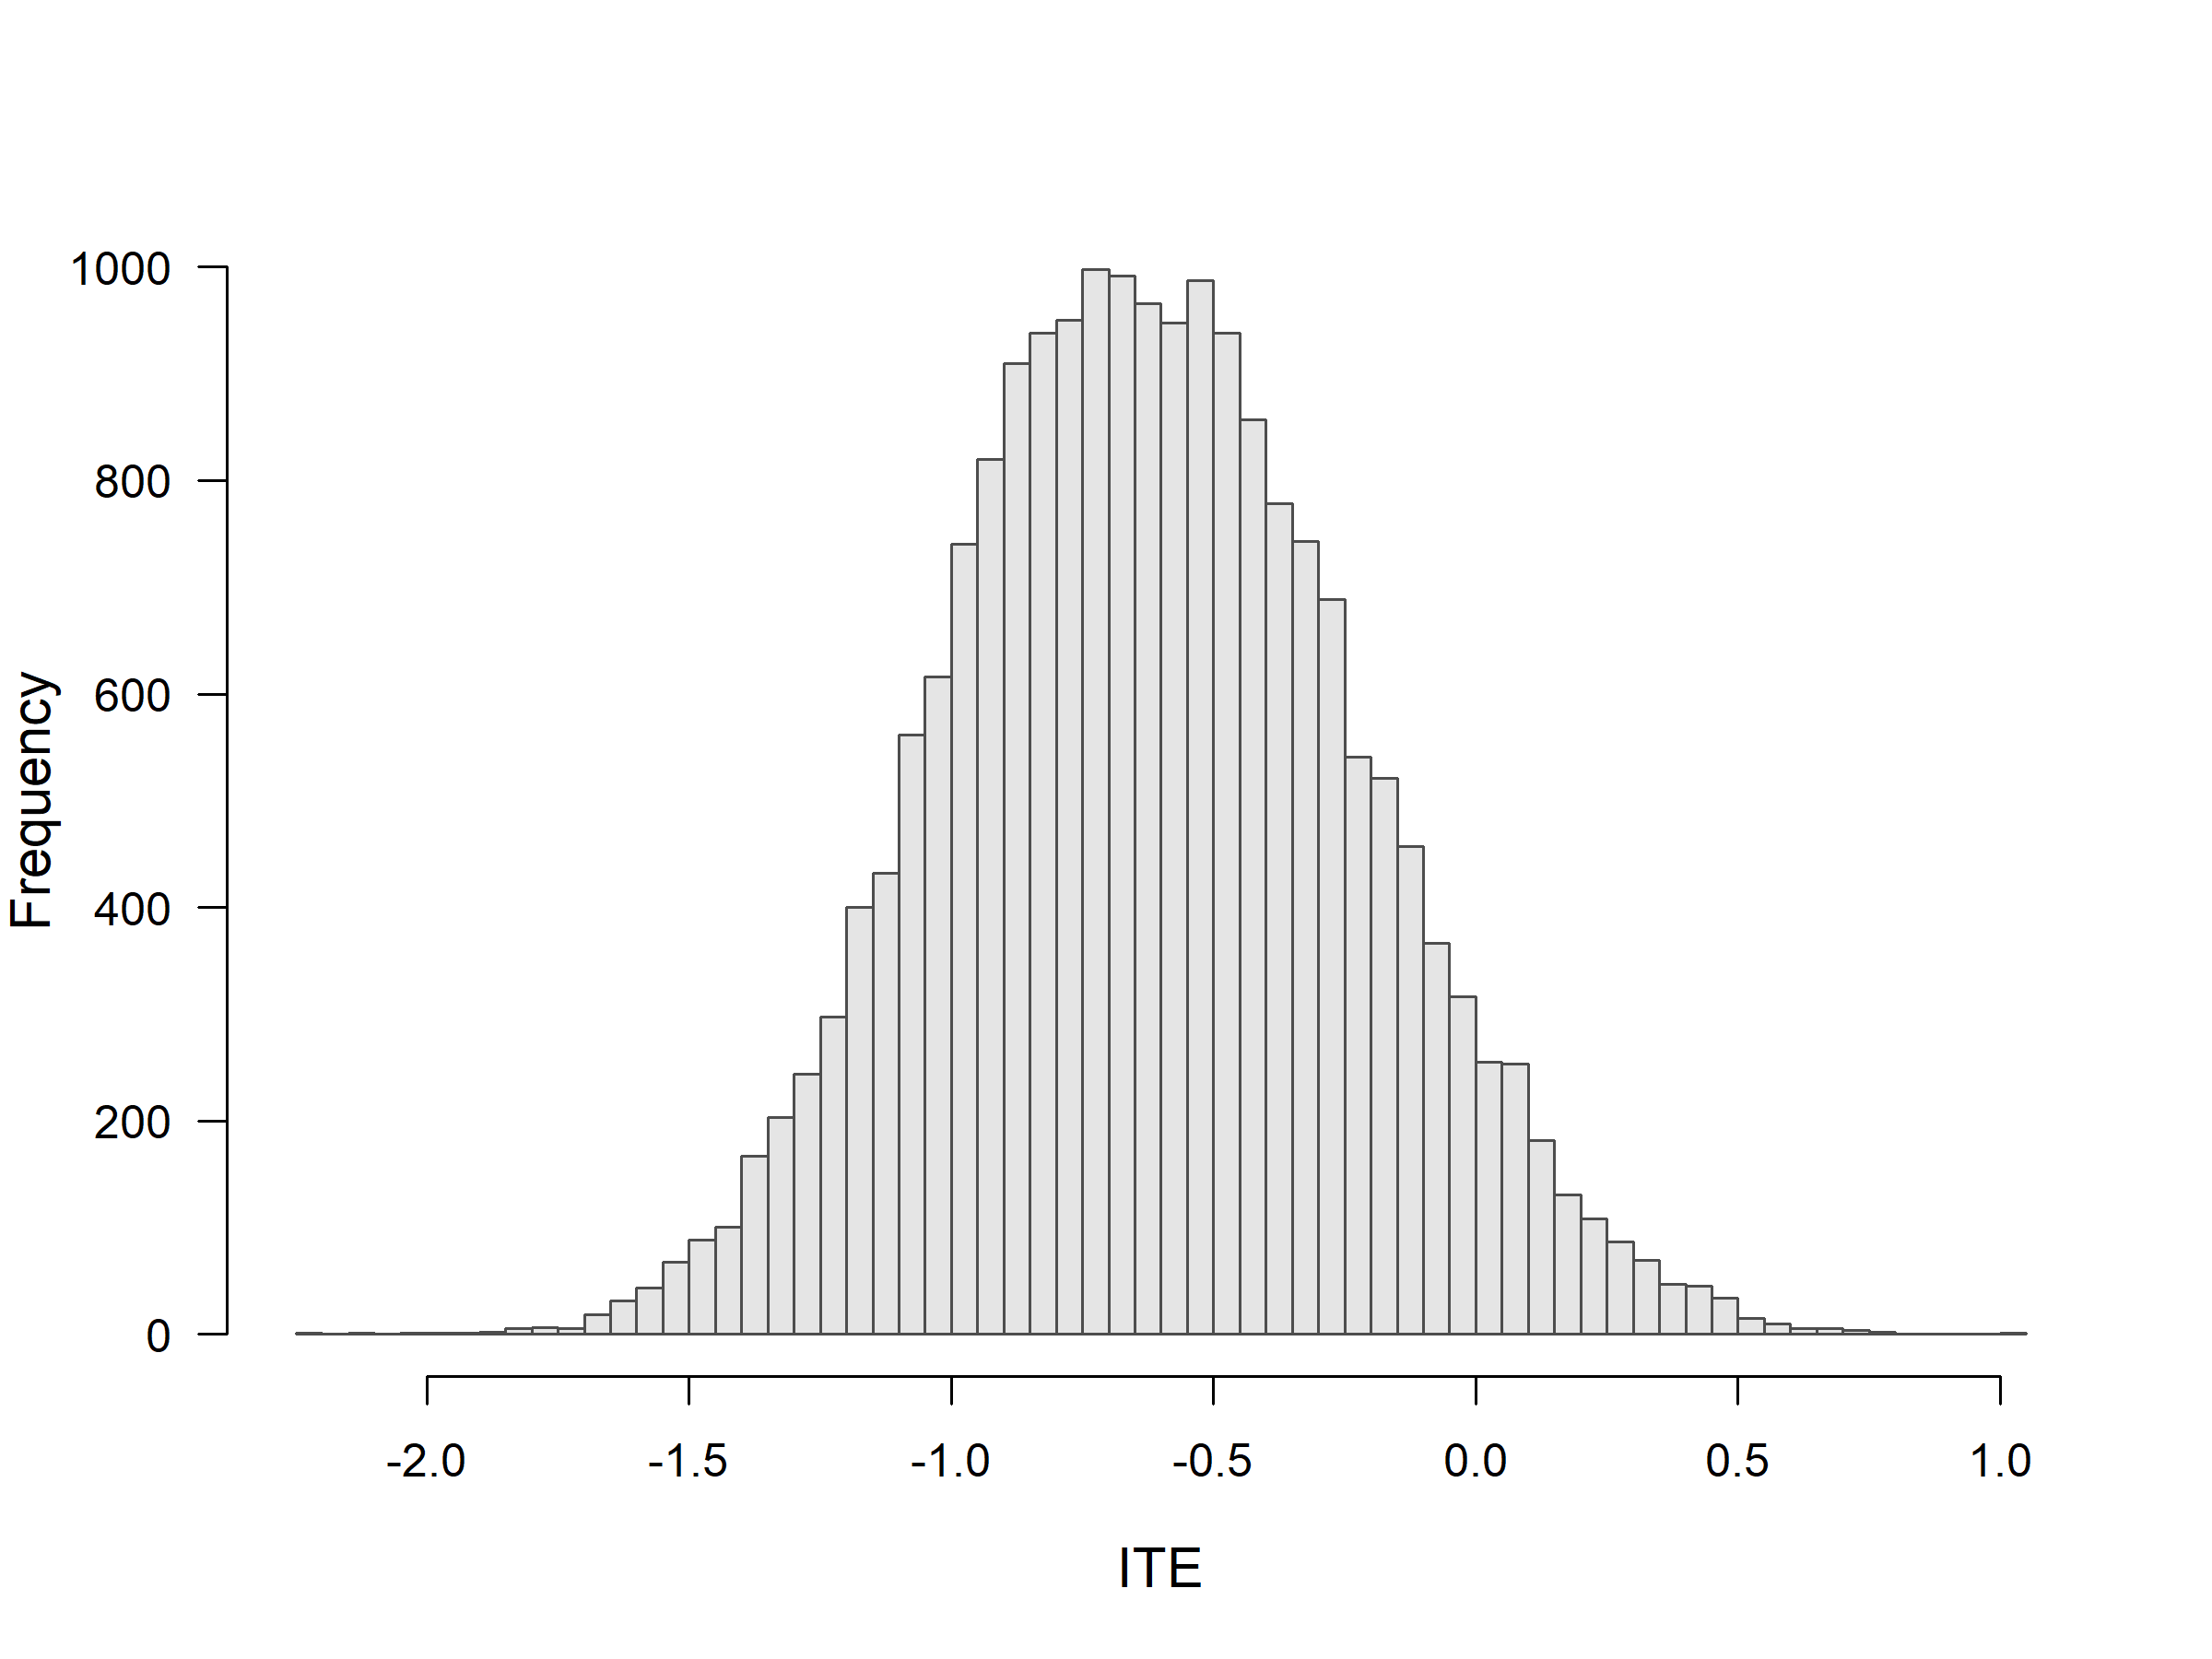
\includegraphics[width=0.45\textwidth]{img/results/rct_scenario1_ite_distribution_dgp.png}
\caption{True ITE distribution resulting from the DGP for scenario (1) with direct and interaction effects. The true ITEs are identical in the observational and in the RCT setting, since they depend on the potential outcomes under both treatment allocations. Left: Observational; Right: RCT setting.}
\label{fig:scenario1_ite_distribution_dgp}
\end{figure}



\begin{figure}[htbp]
\centering
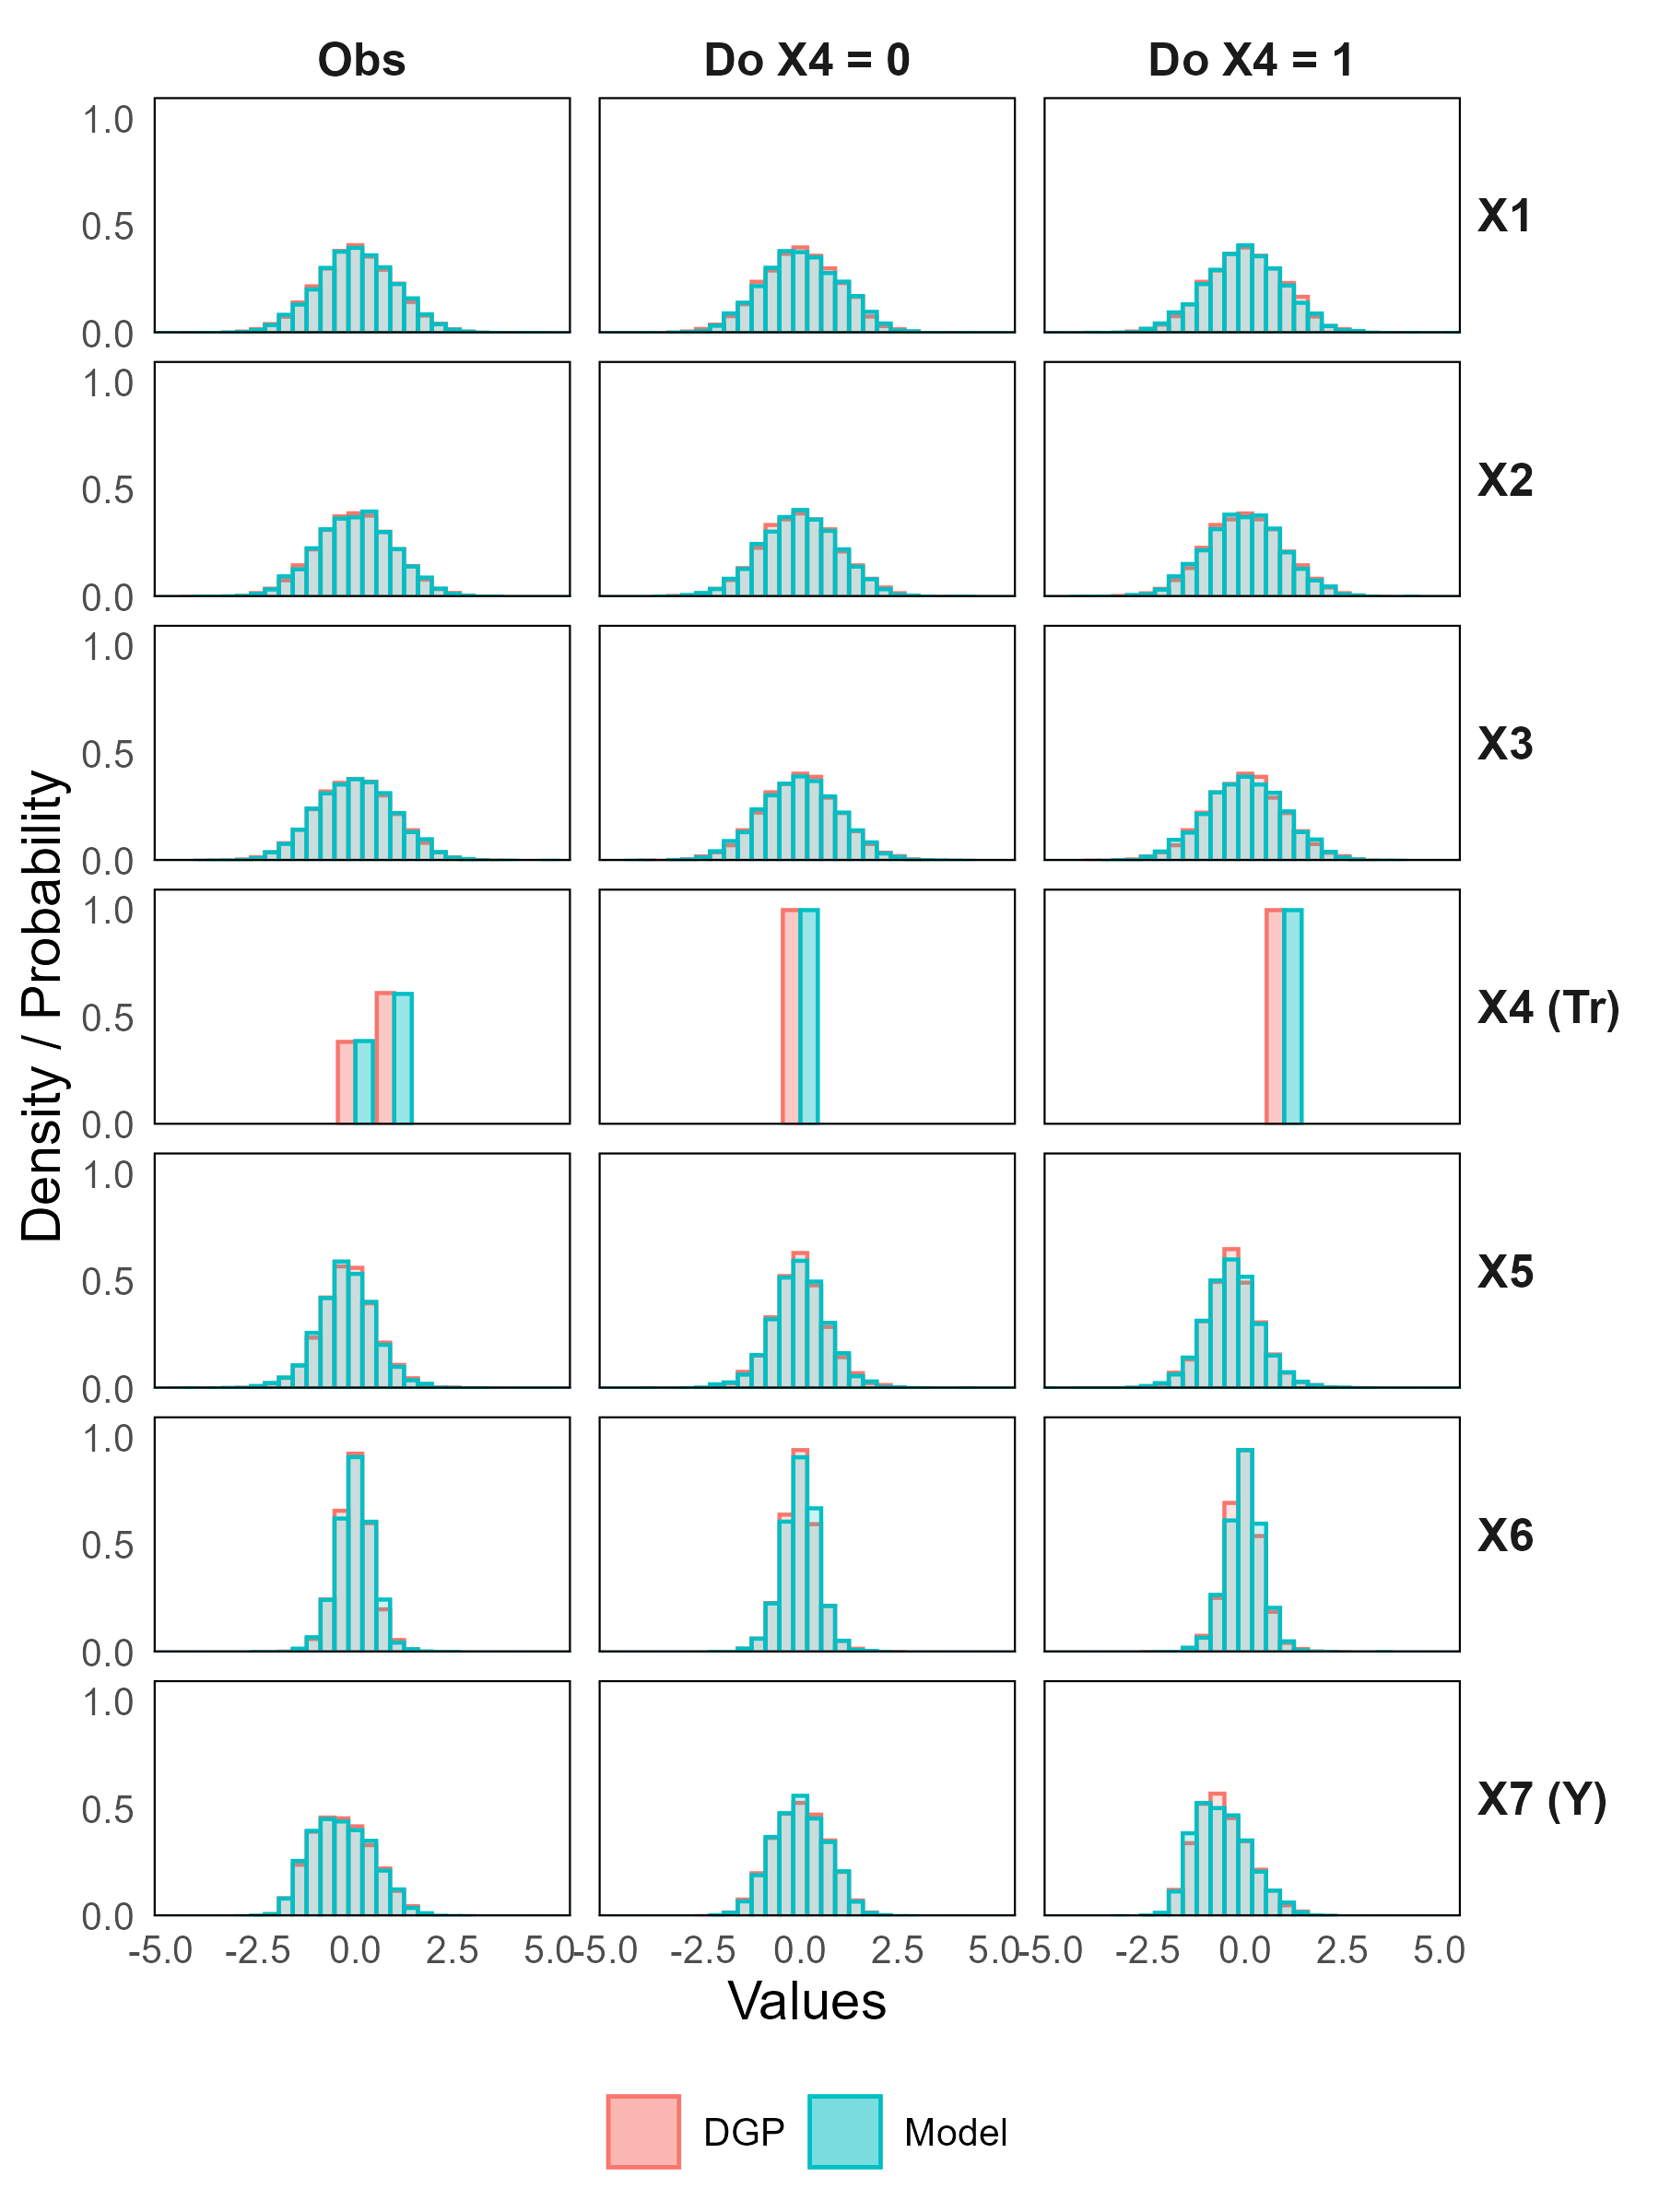
\includegraphics[width=0.45\textwidth]{img/results/observ_scenario1_sampling_distributions_vertical.png}
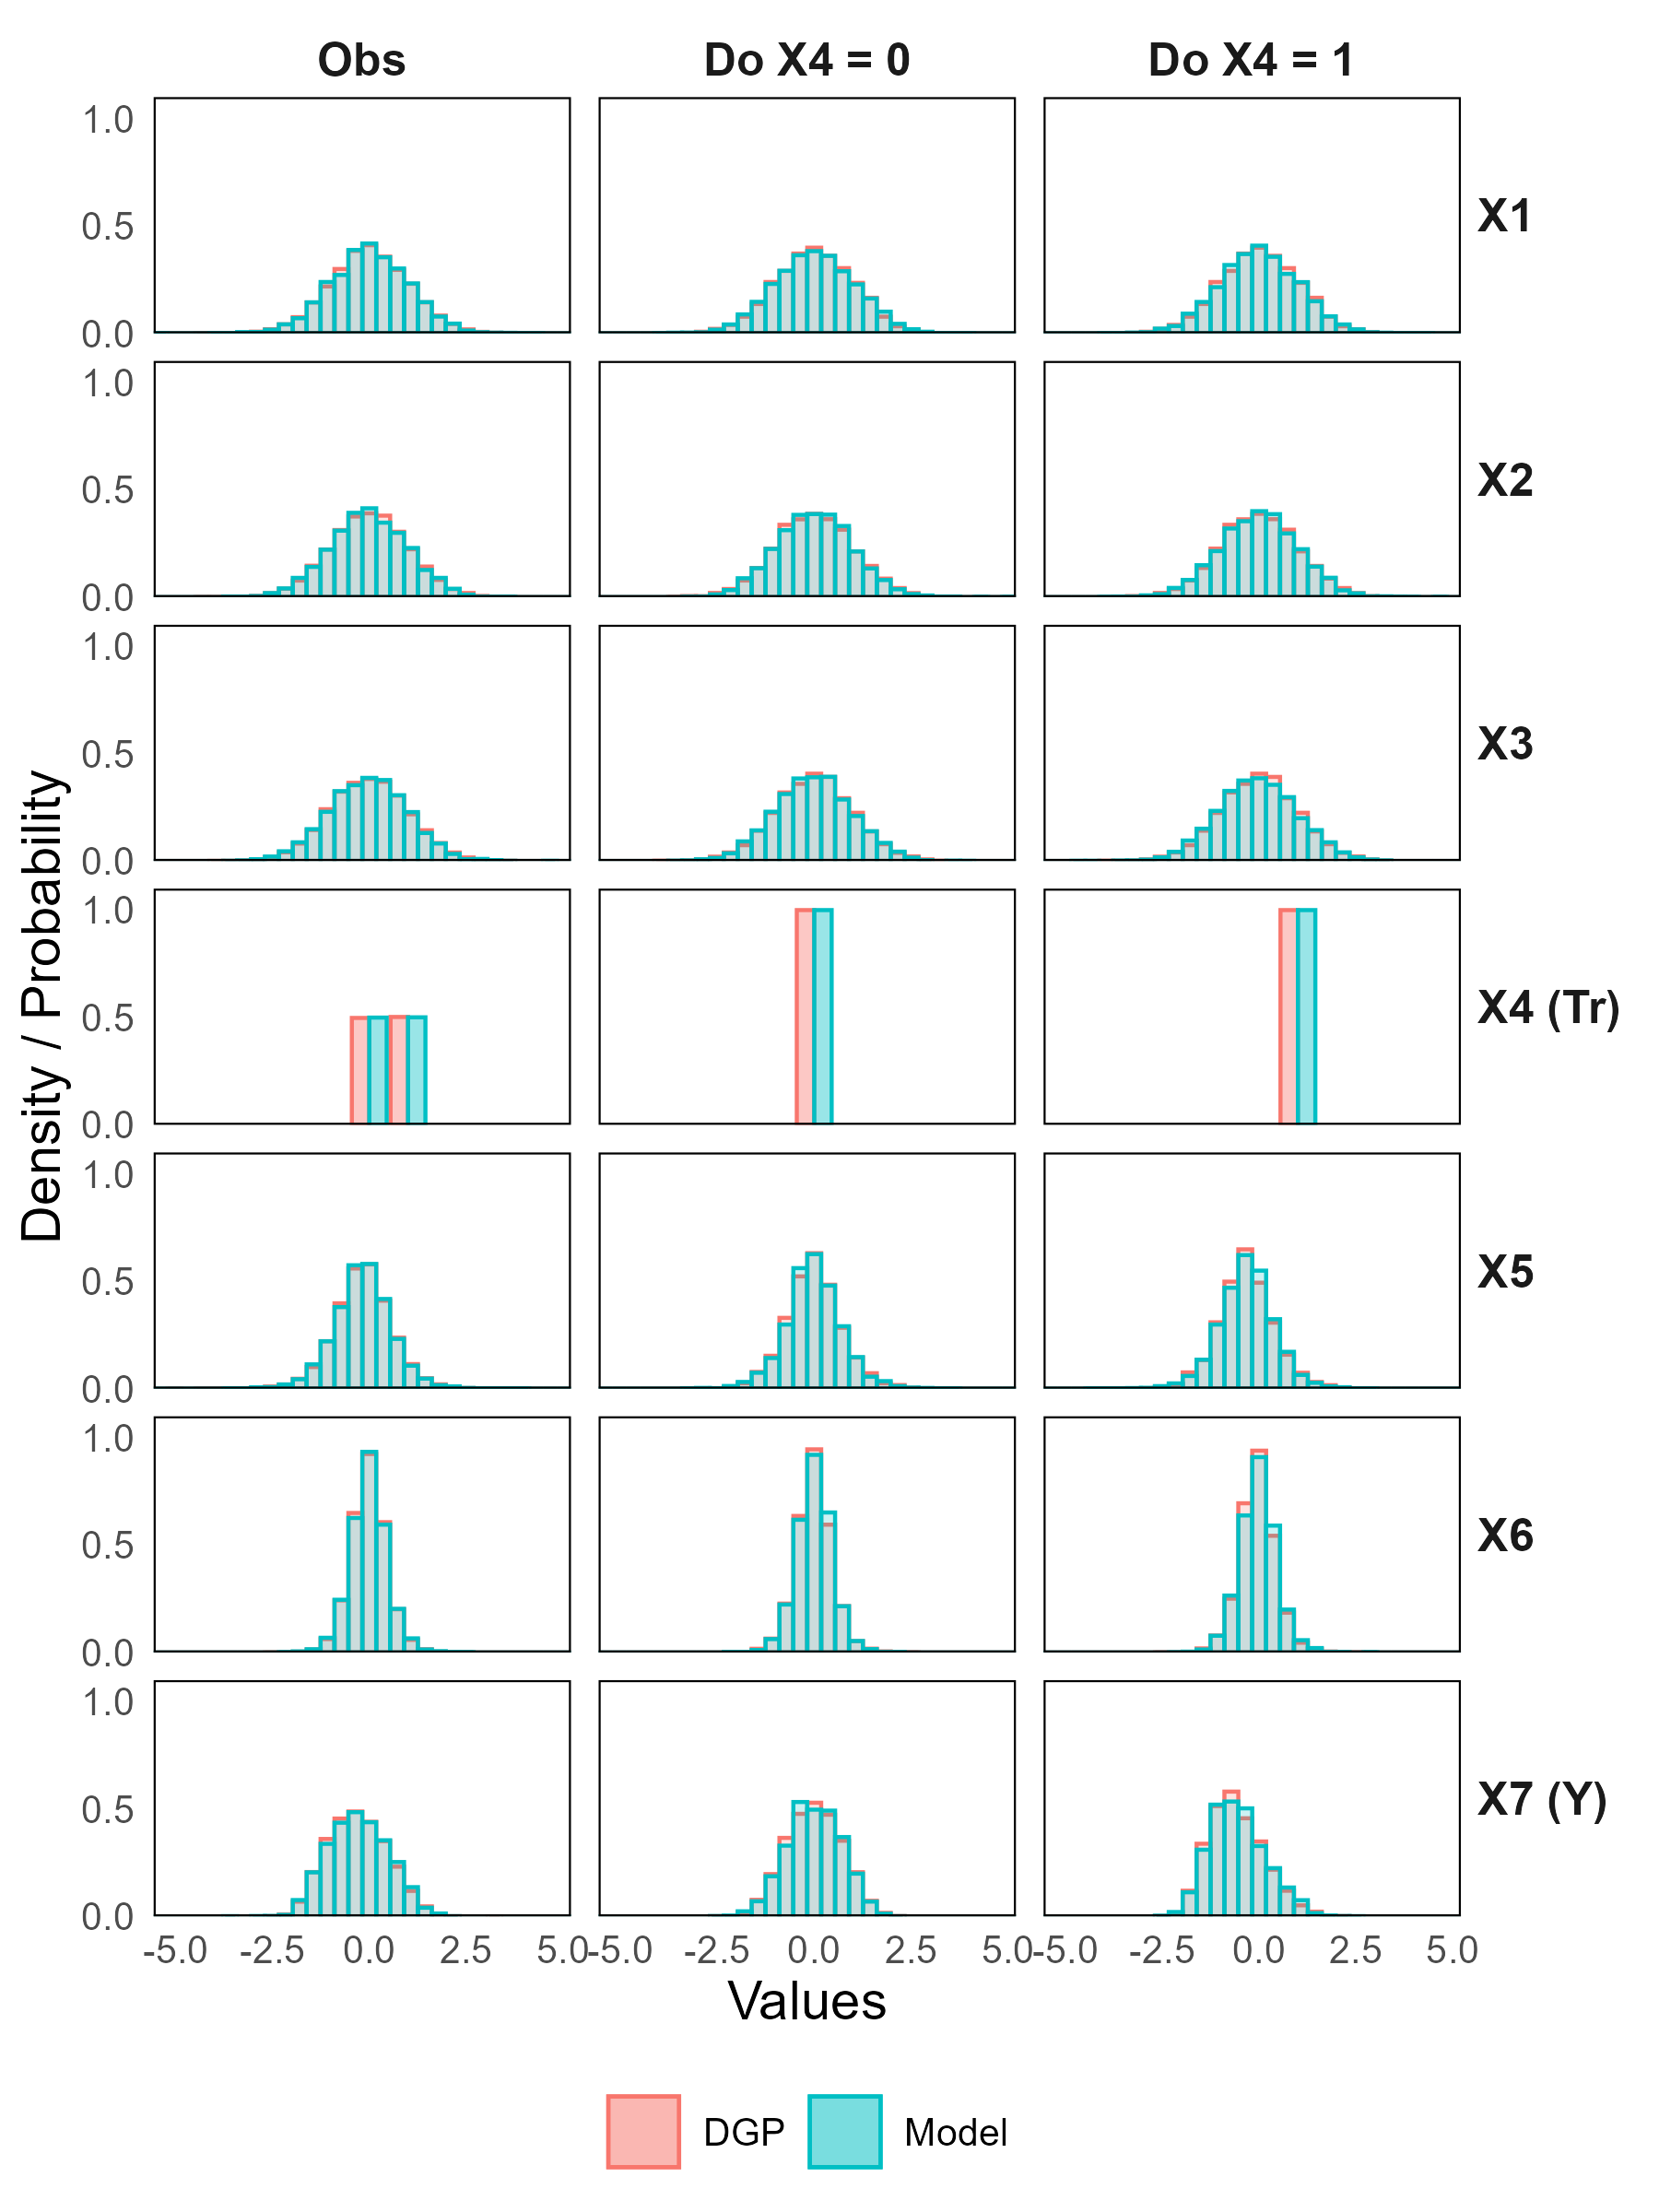
\includegraphics[width=0.45\textwidth]{img/results/rct_scenario1_sampling_distributions_vertical.png}
\caption{Marginal distributions of DGP variables and fitted TRAM-DAG samples for scenario (1) with direct and interaction effects. The distributions shown as observed (Obs), under control intervention (Do $X4=0$) and under treatment intervention (Do $X4=1$). Left: Observational; Right: RCT setting.}
\label{fig:scenario1_sampling_distributions_vertical}
\end{figure}

\begin{figure}[htbp]
\centering
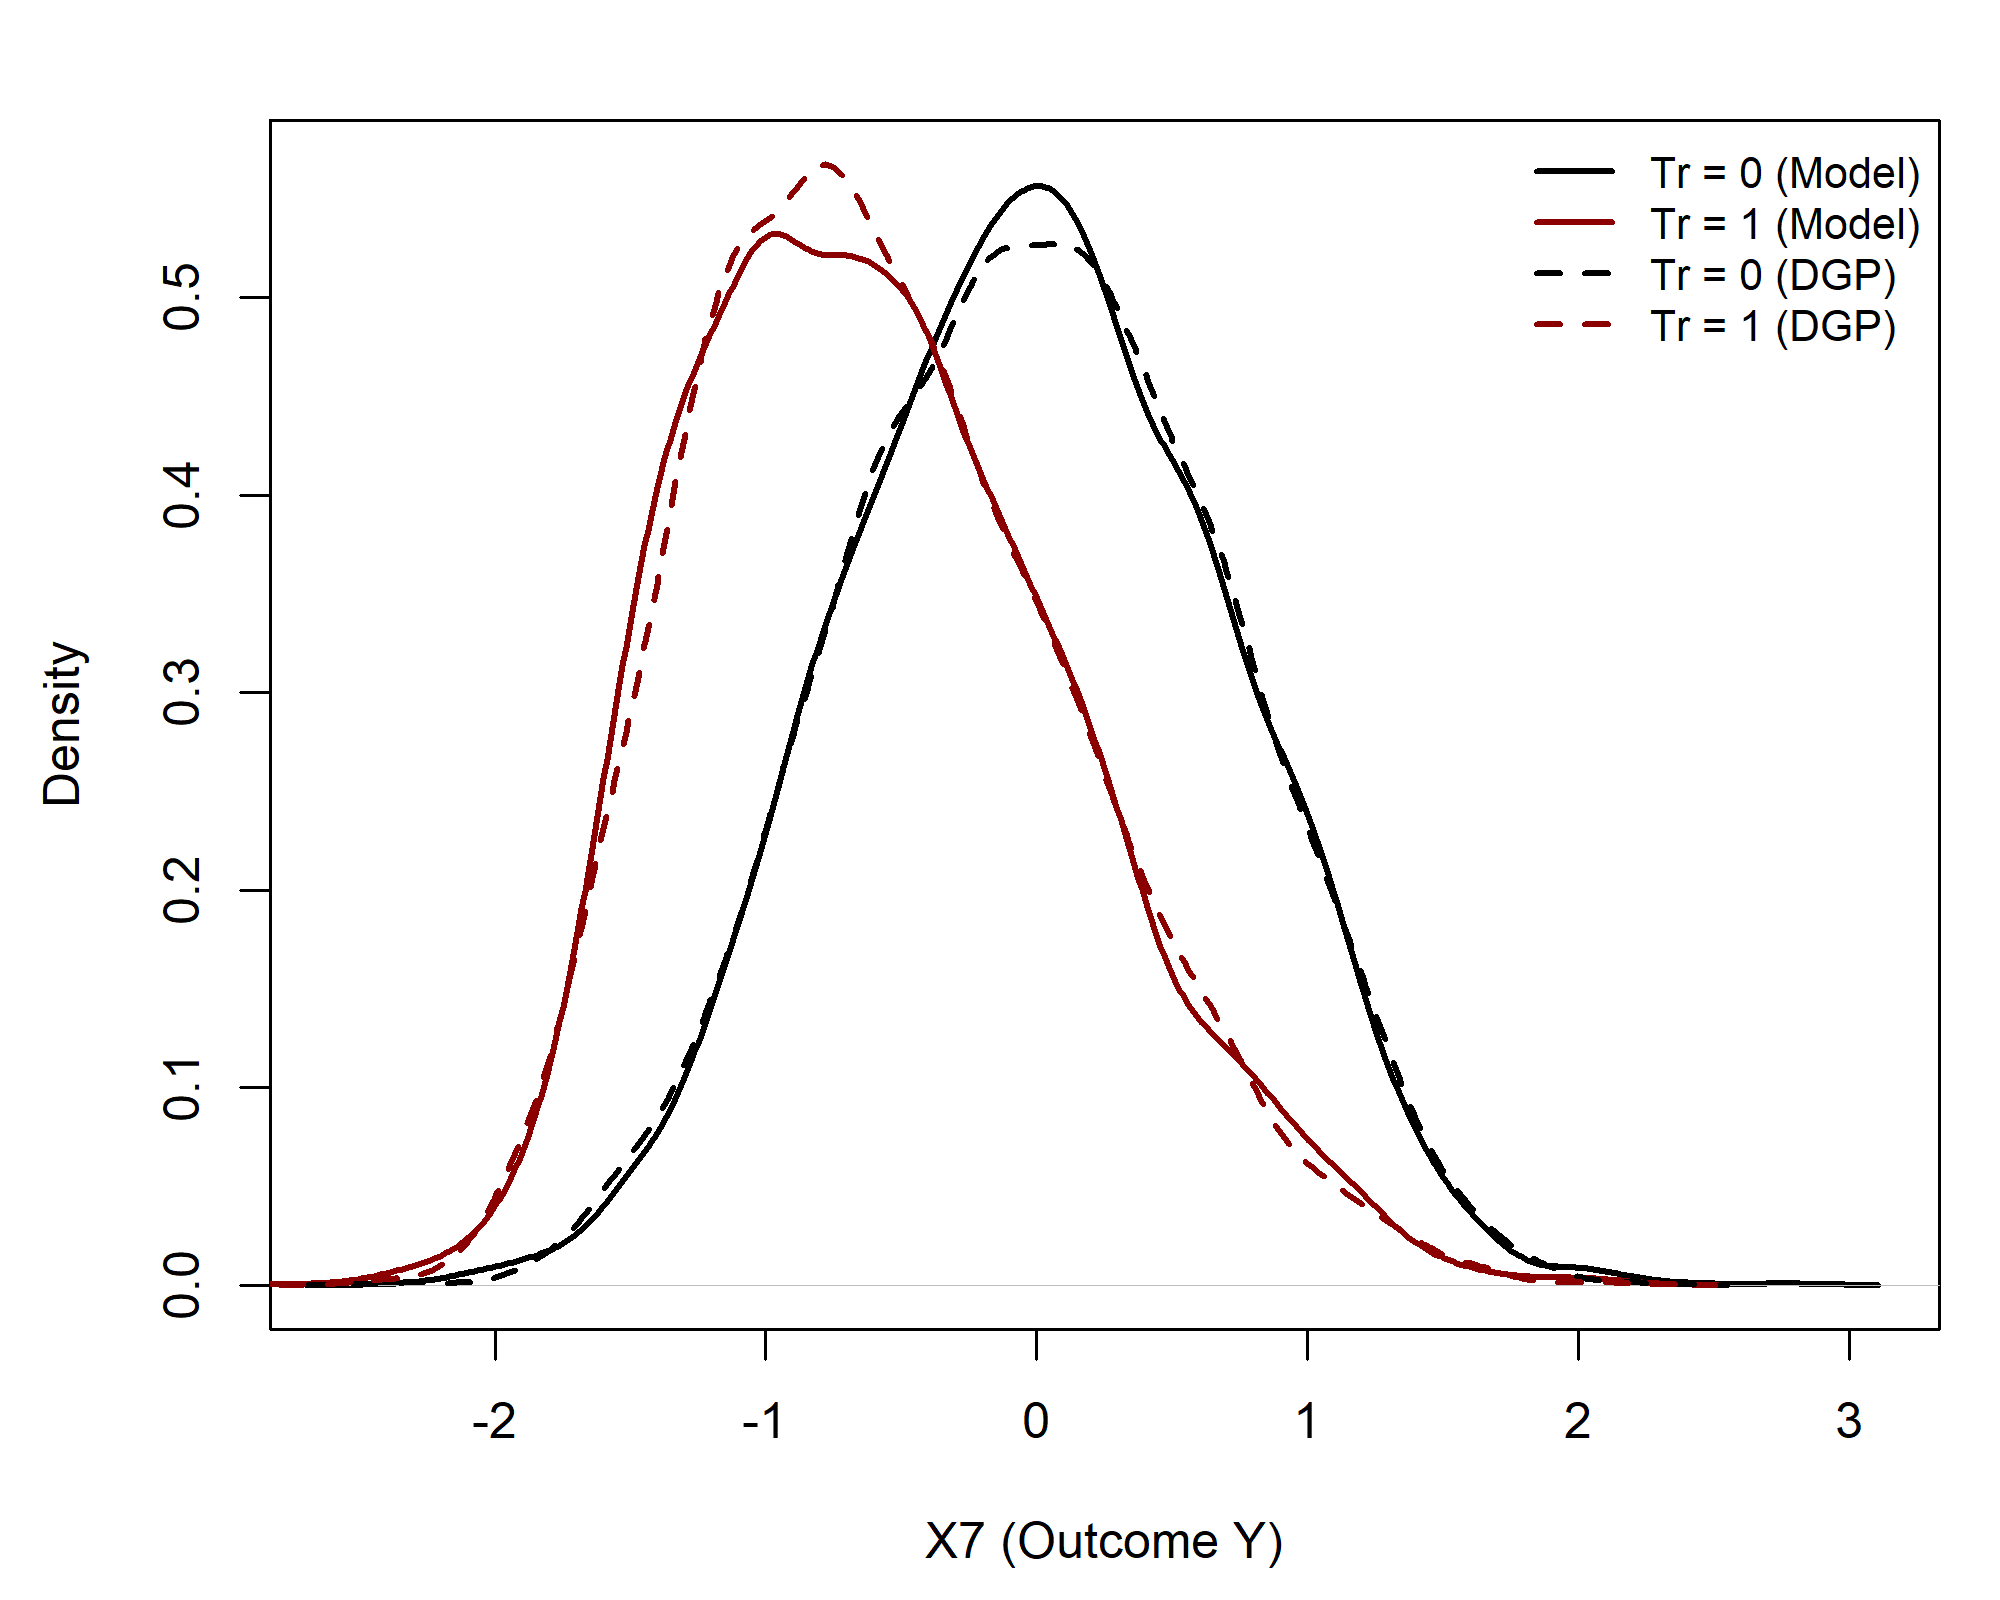
\includegraphics[width=0.45\textwidth]{img/results/observ_scenario1_X7_treatment_densities.png}
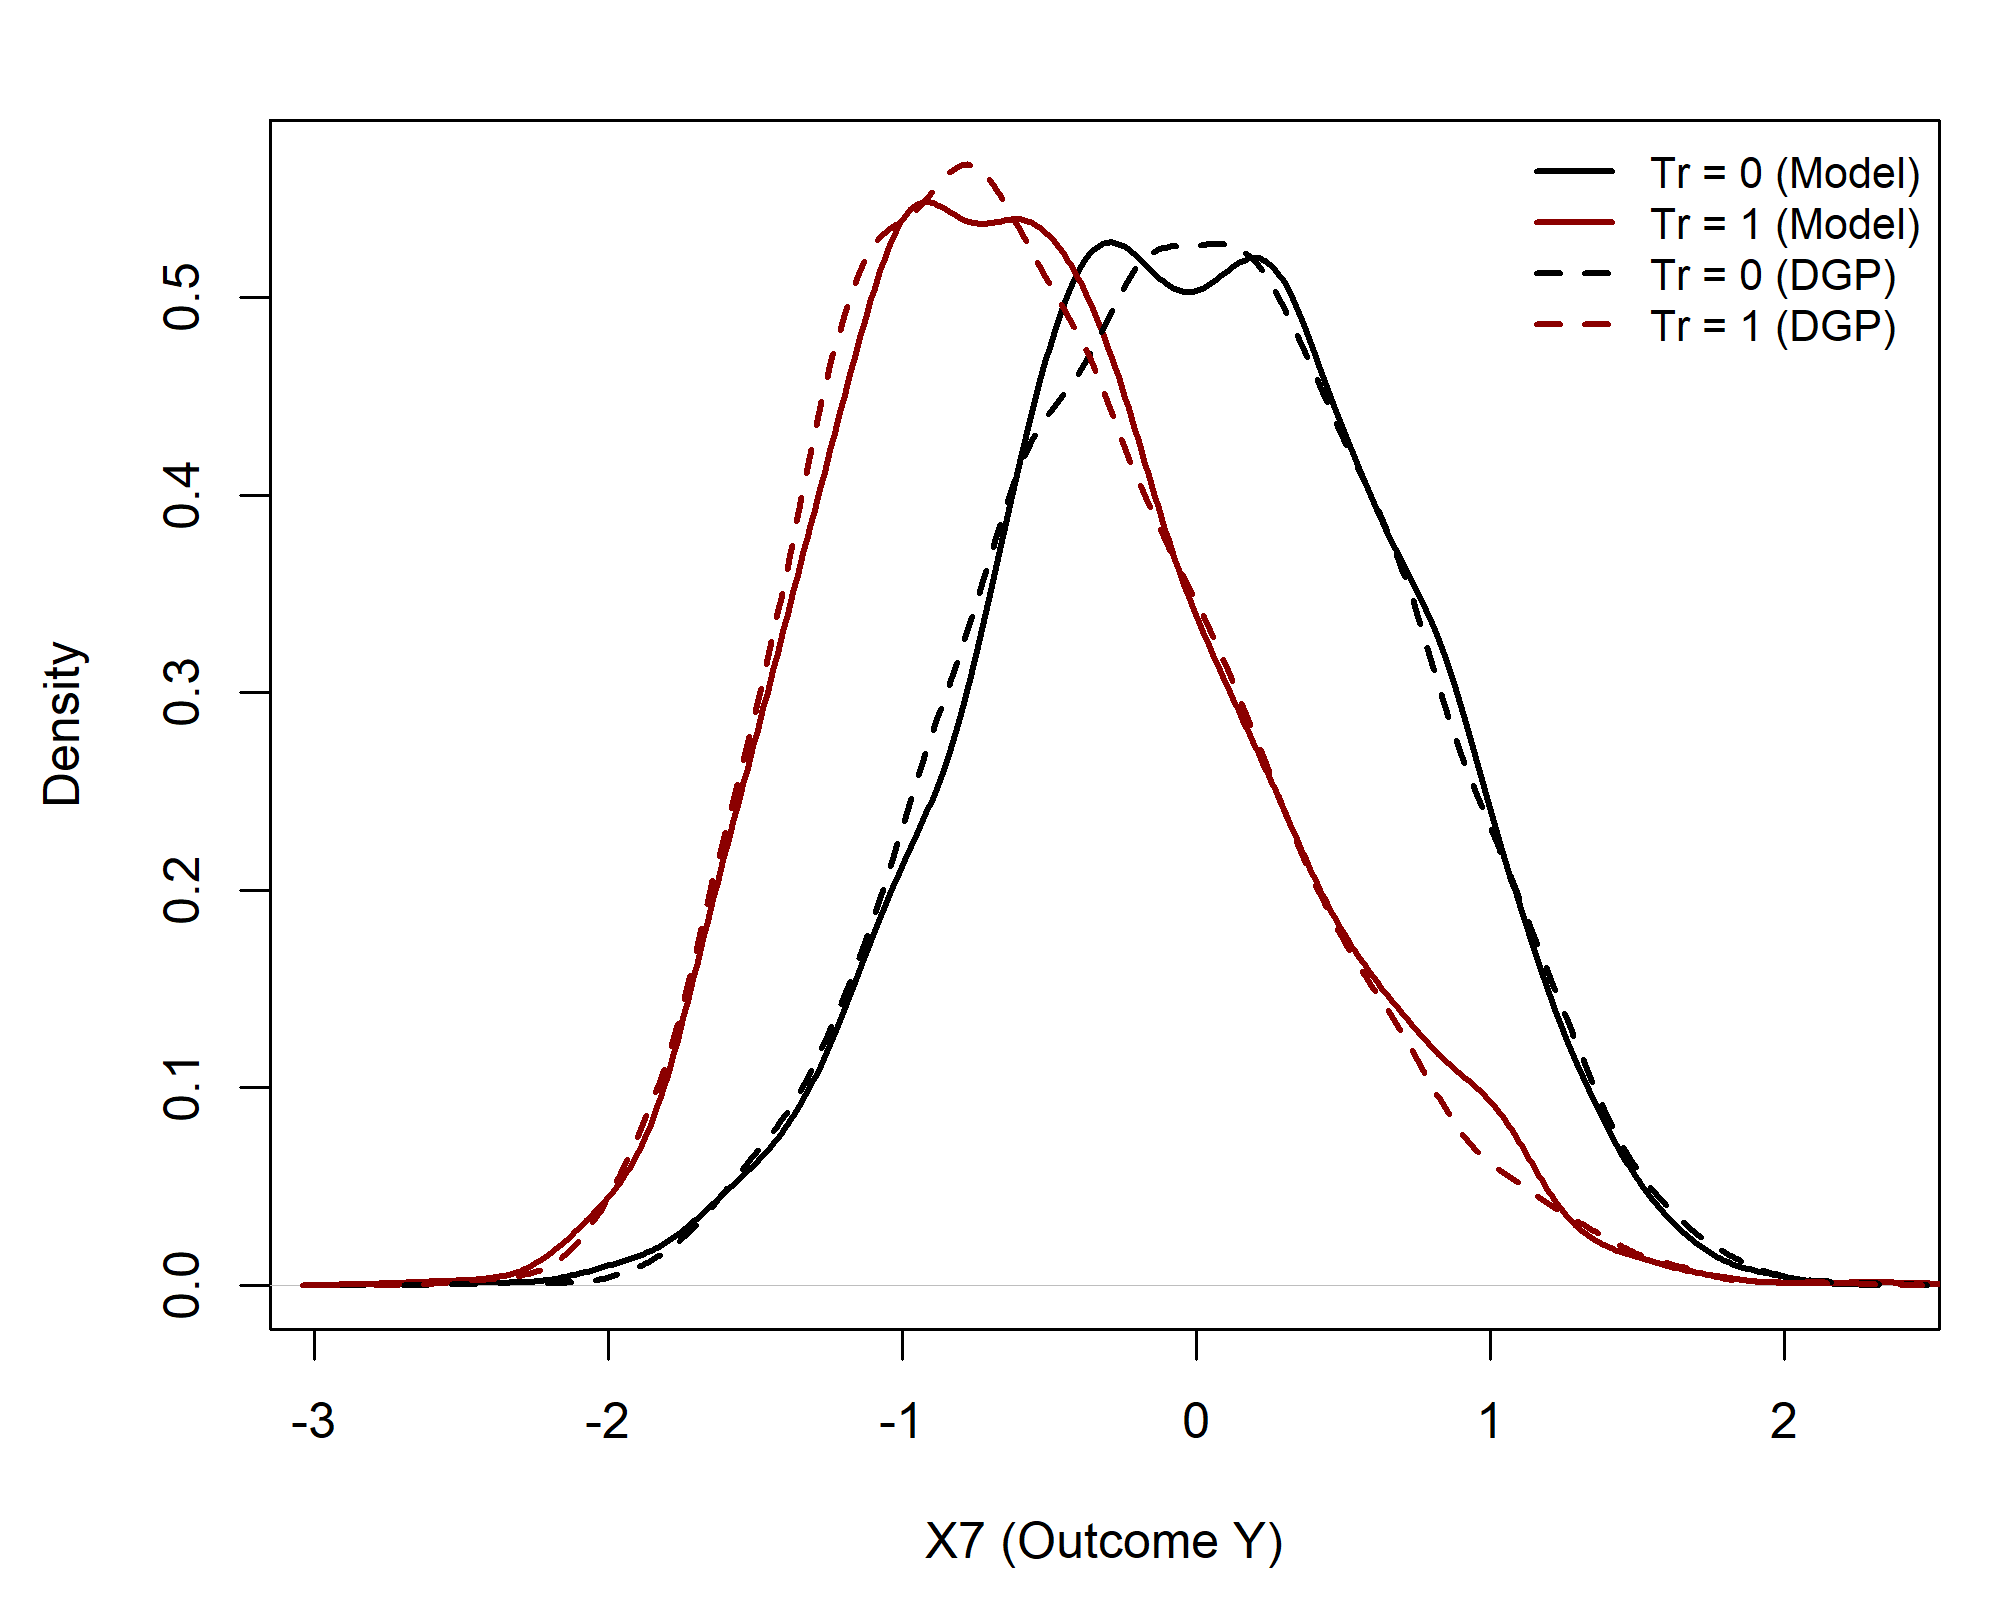
\includegraphics[width=0.45\textwidth]{img/results/rct_scenario1_X7_treatment_densities.png}
\caption{Distributions of the outcome variable (X7) under treatment and control interventions for scenario (1), including direct and interaction effects. This plot is a higher resolution view of the X7 panels (Do $X4=0$) and (Do $X4=1$) from Figure \ref{fig:scenario1_sampling_distributions_vertical}. Left: Observational; Right: RCT setting.}
\label{fig:scenario1_outcome_distributions}
\end{figure}




\begin{figure}[htbp]
\centering
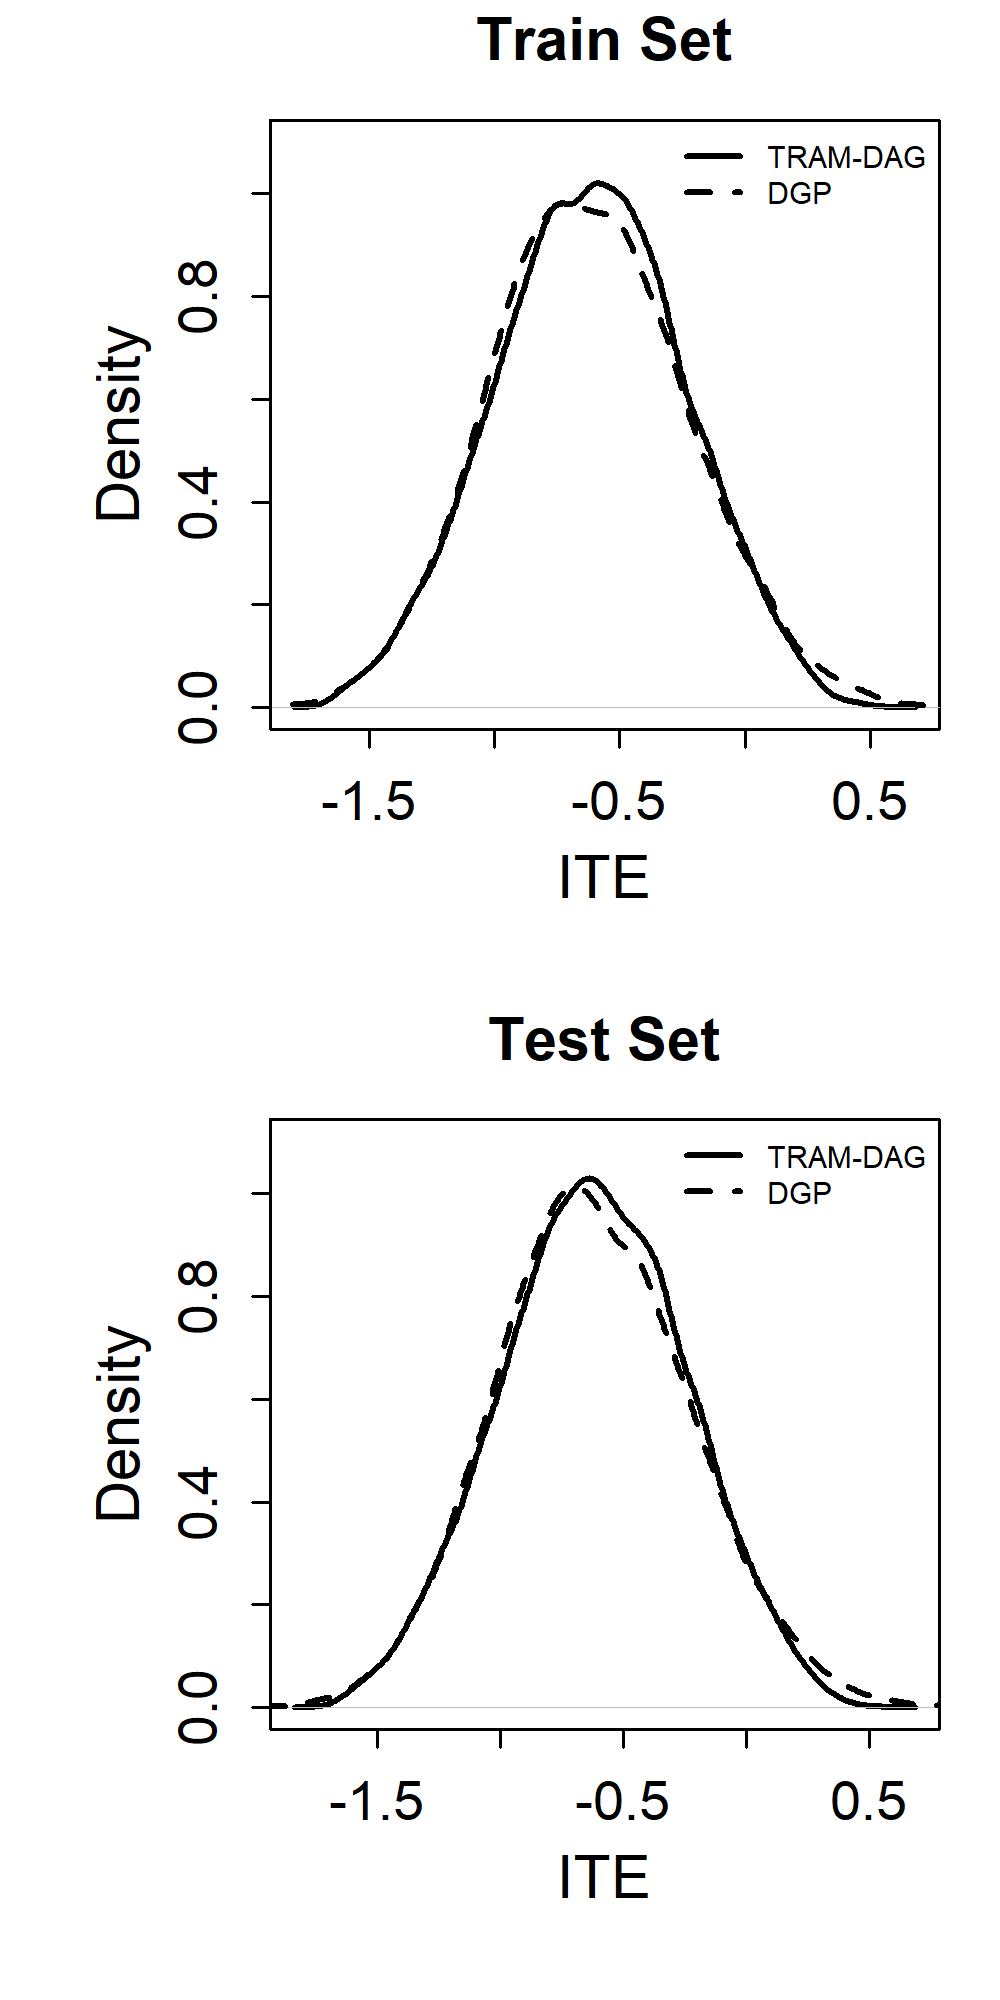
\includegraphics[width=0.45\textwidth]{img/results/observ_scenario1_ITE_densities_train_test.png}
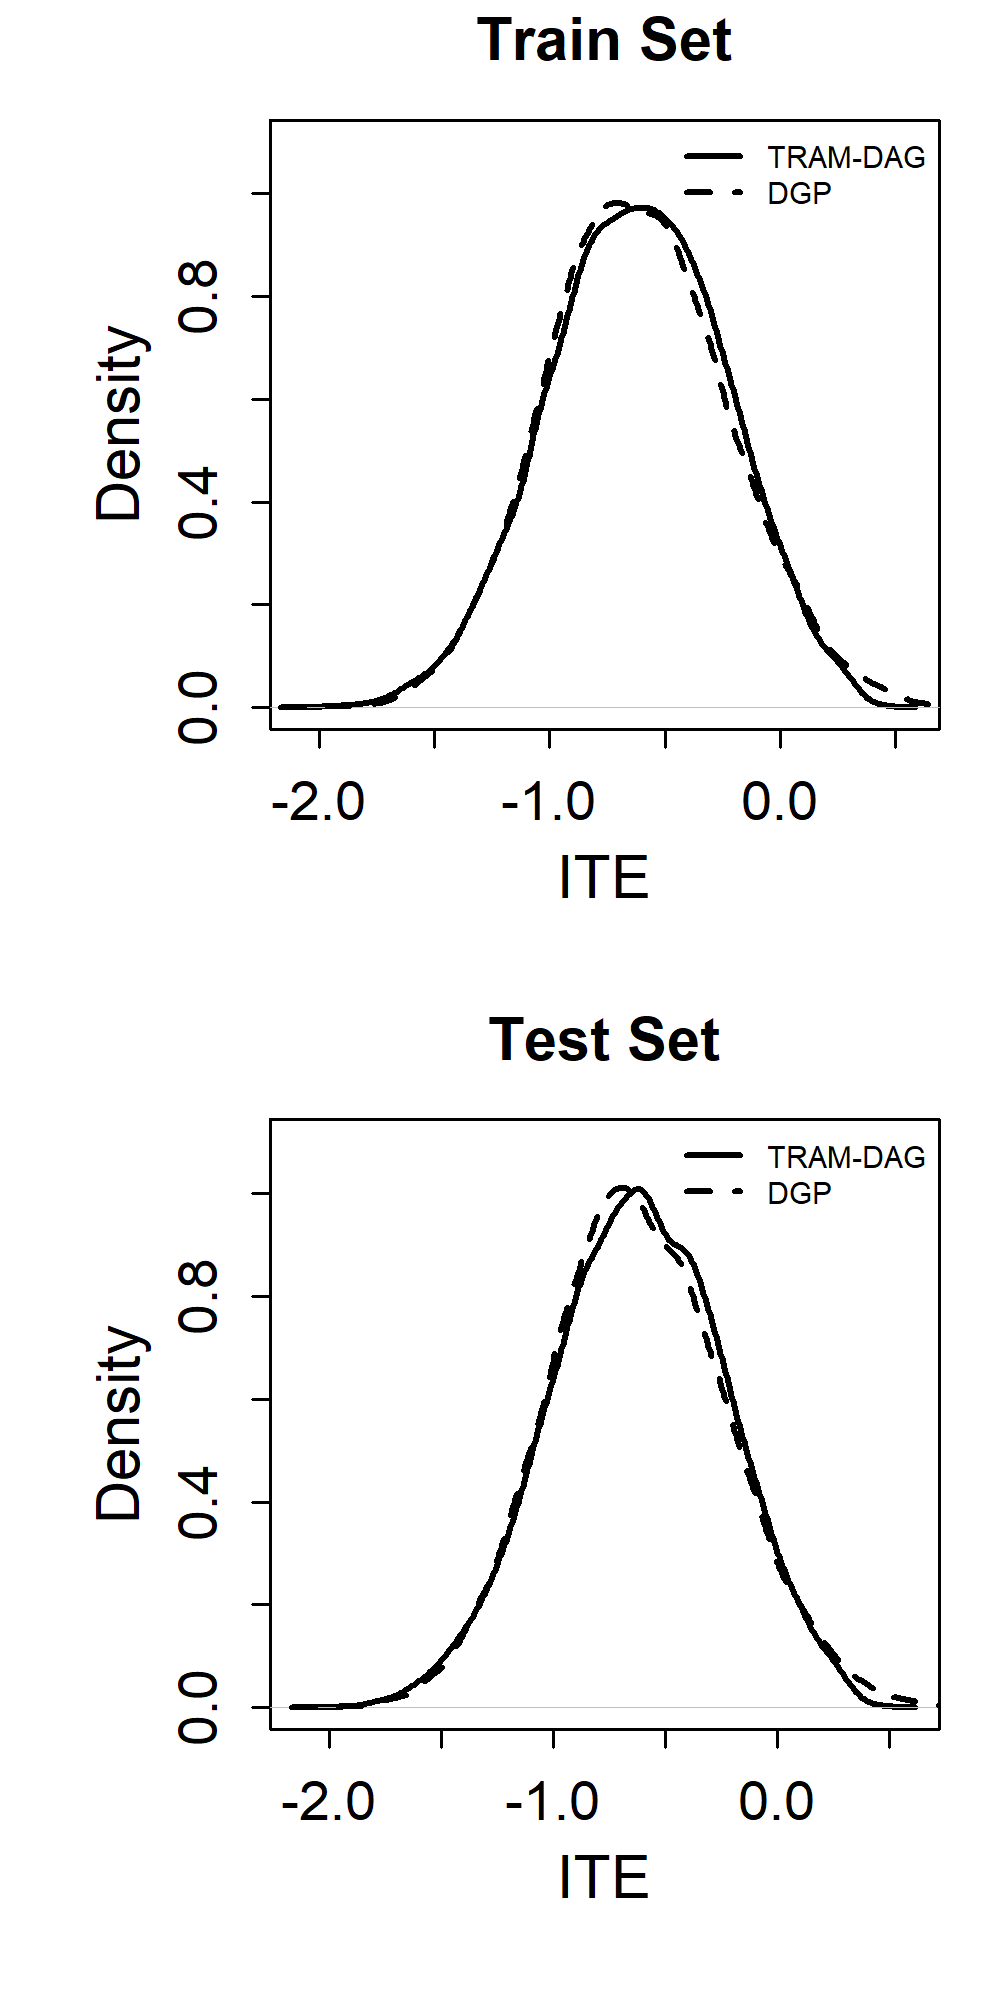
\includegraphics[width=0.45\textwidth]{img/results/rct_scenario1_ITE_densities_train_test.png}
\caption{Densities of estimated ITEs compared to the true ITEs in the training and test datasets for scenario (1), including direct and interaction effects. Left: Observational; right: RCT setting.}
\label{fig:scenario1_ite_densities_train_test}
\end{figure}






\begin{figure}[htbp]
\centering
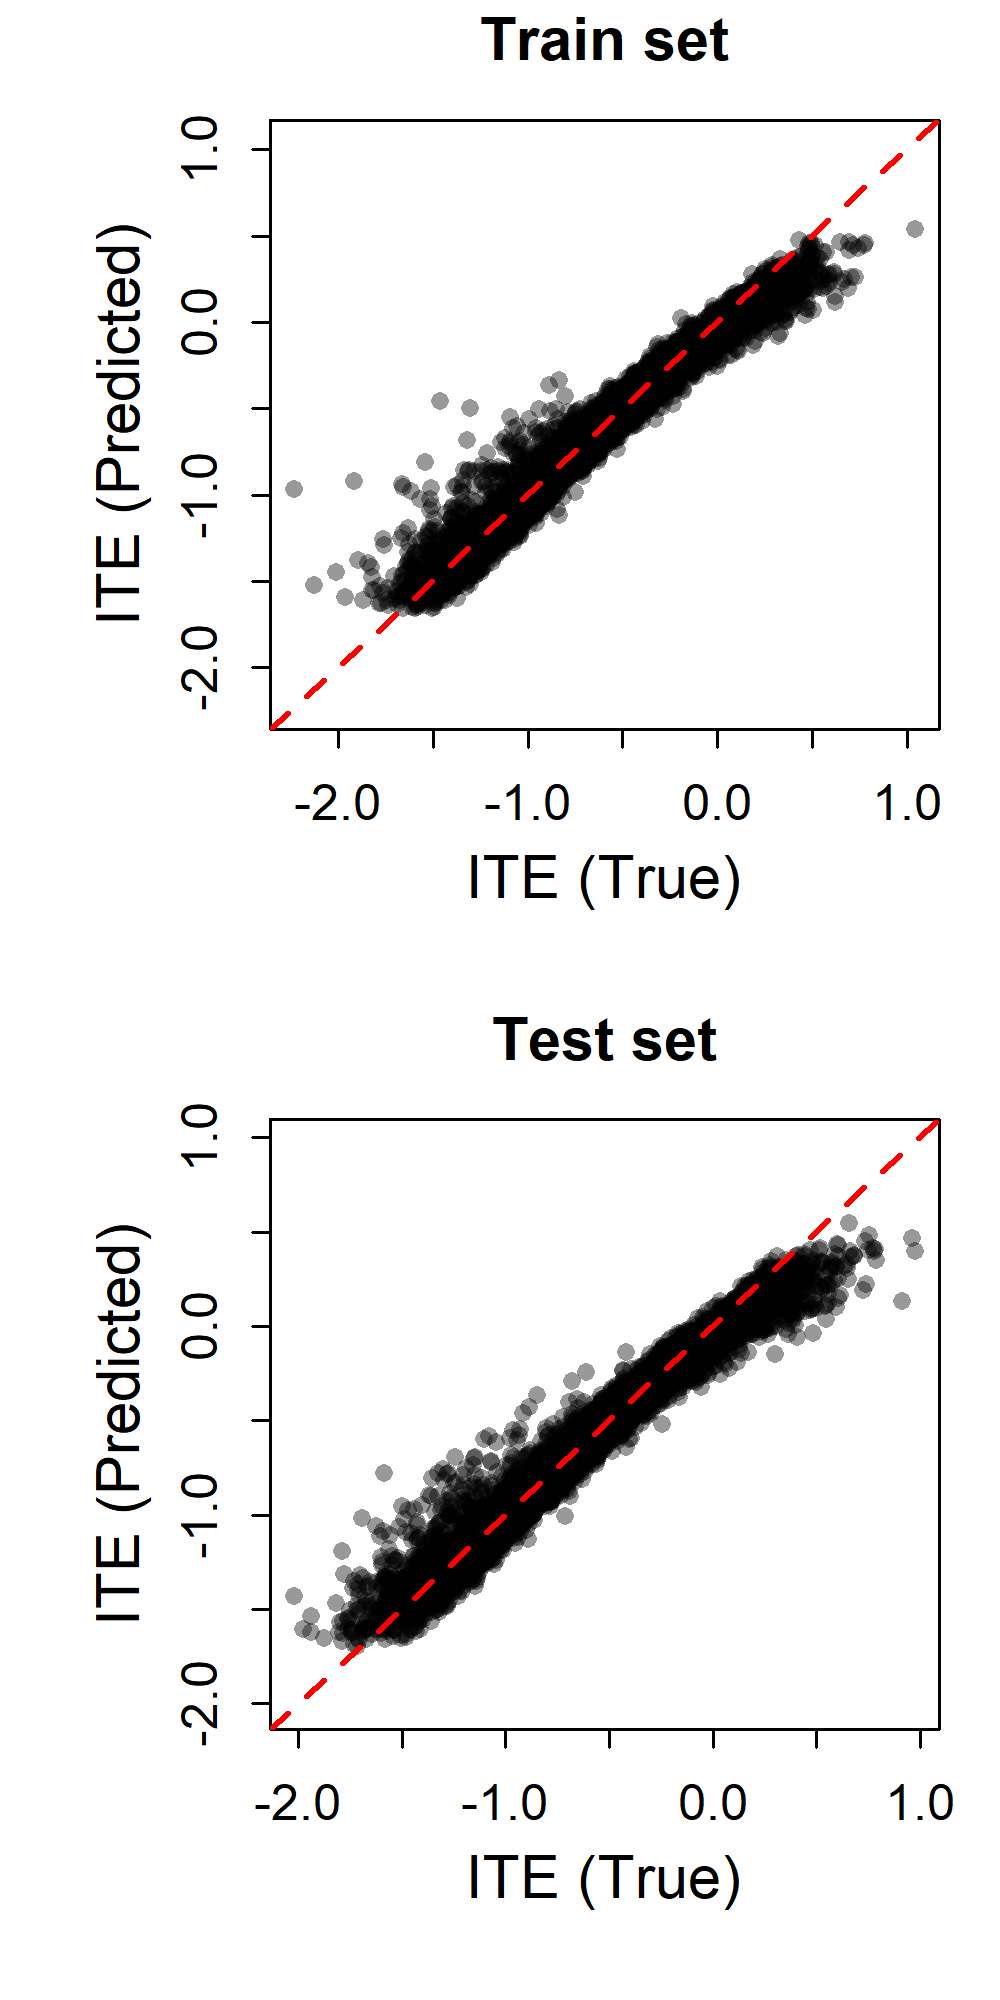
\includegraphics[width=0.45\textwidth]{img/results/observ_scenario1_ITE_scatter_train_test.png}
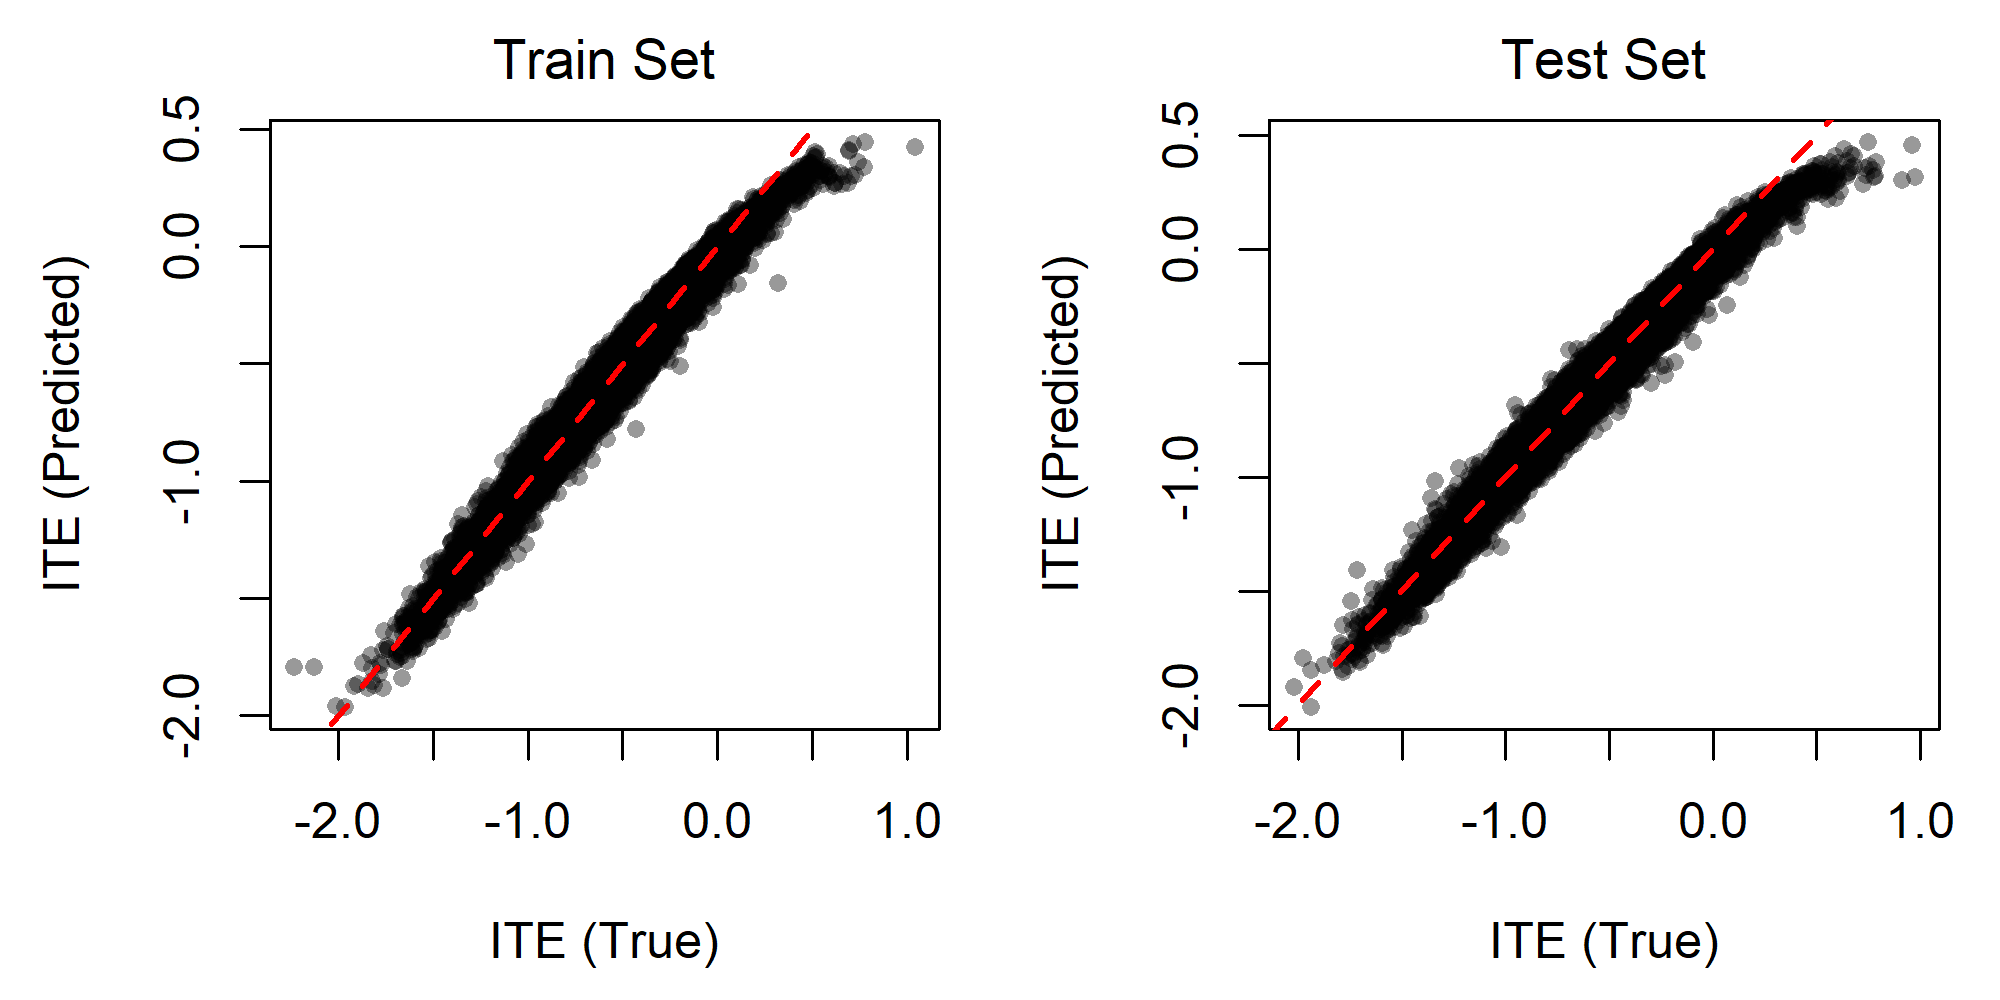
\includegraphics[width=0.45\textwidth]{img/results/rct_scenario1_ITE_scatter_train_test.png}
\caption{Scatterplots of estimated ITEs compared to the true ITEs in the training and test datasets for scenario (1), including direct and interaction effects. Left: Observational; right: RCT setting.}
\label{fig:scenario1_ite_scatter_train_test}
\end{figure}




\begin{figure}[htbp]
\centering
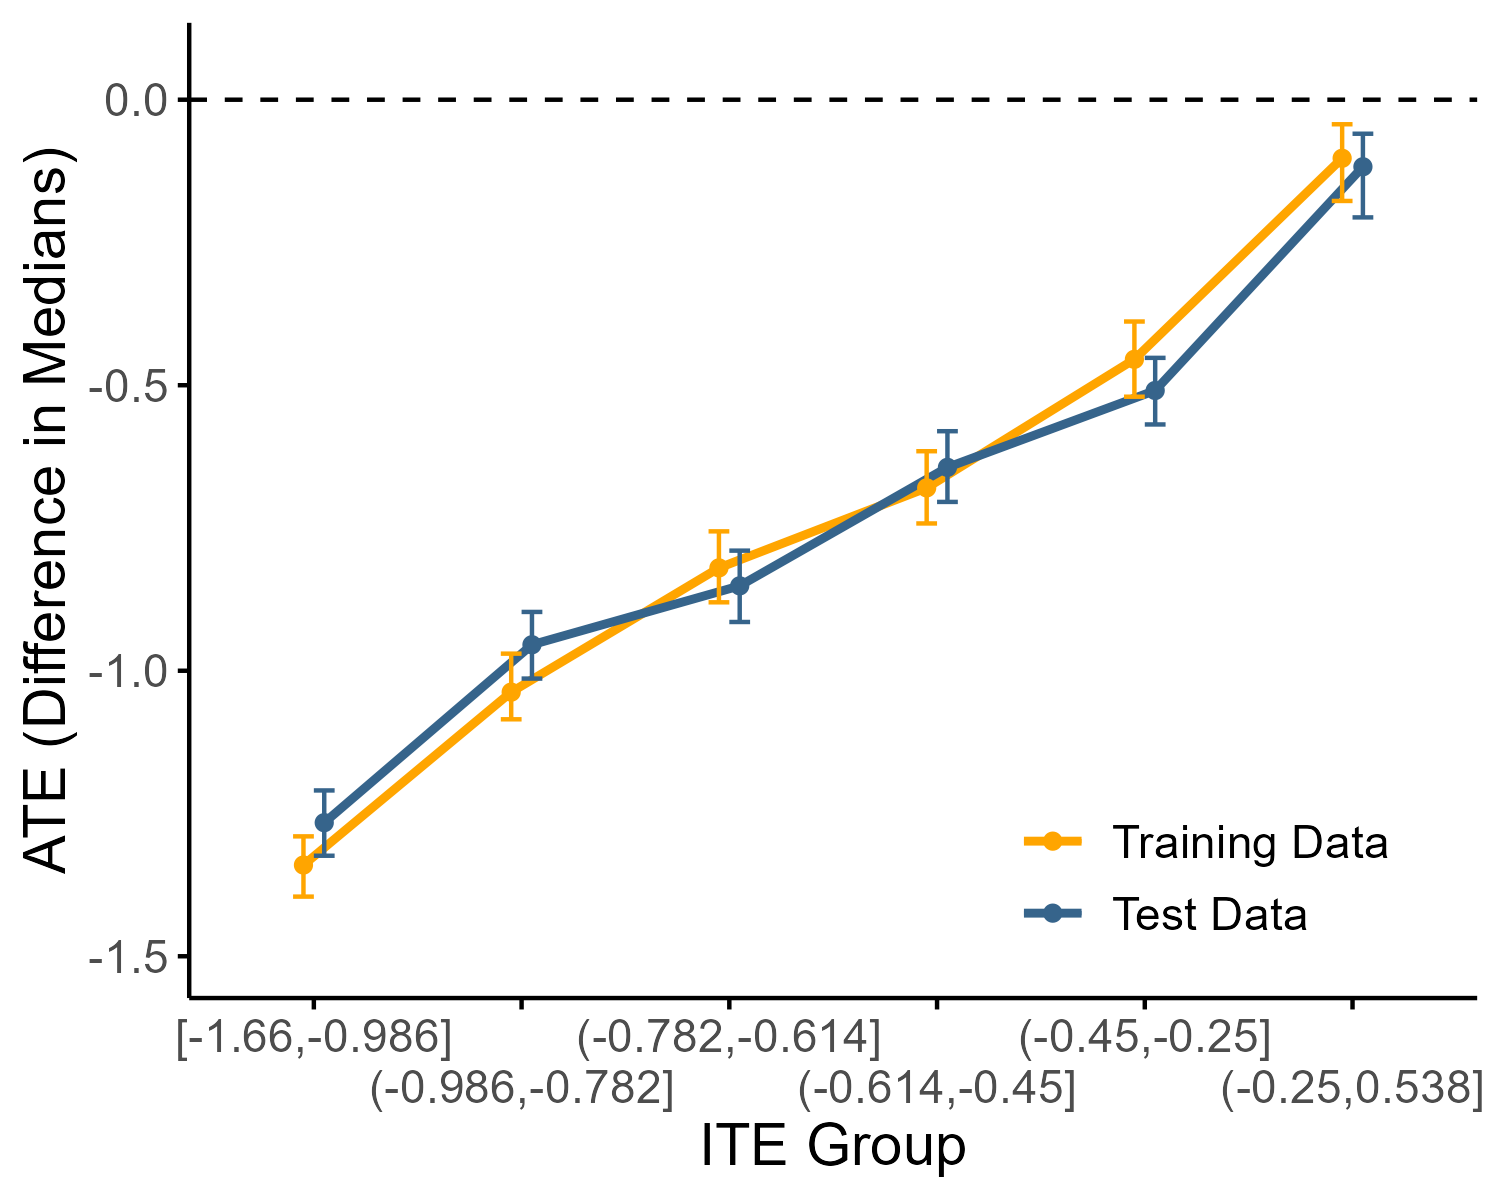
\includegraphics[width=0.45\textwidth]{img/results/observ_scenario1_ITE_cATE.png}
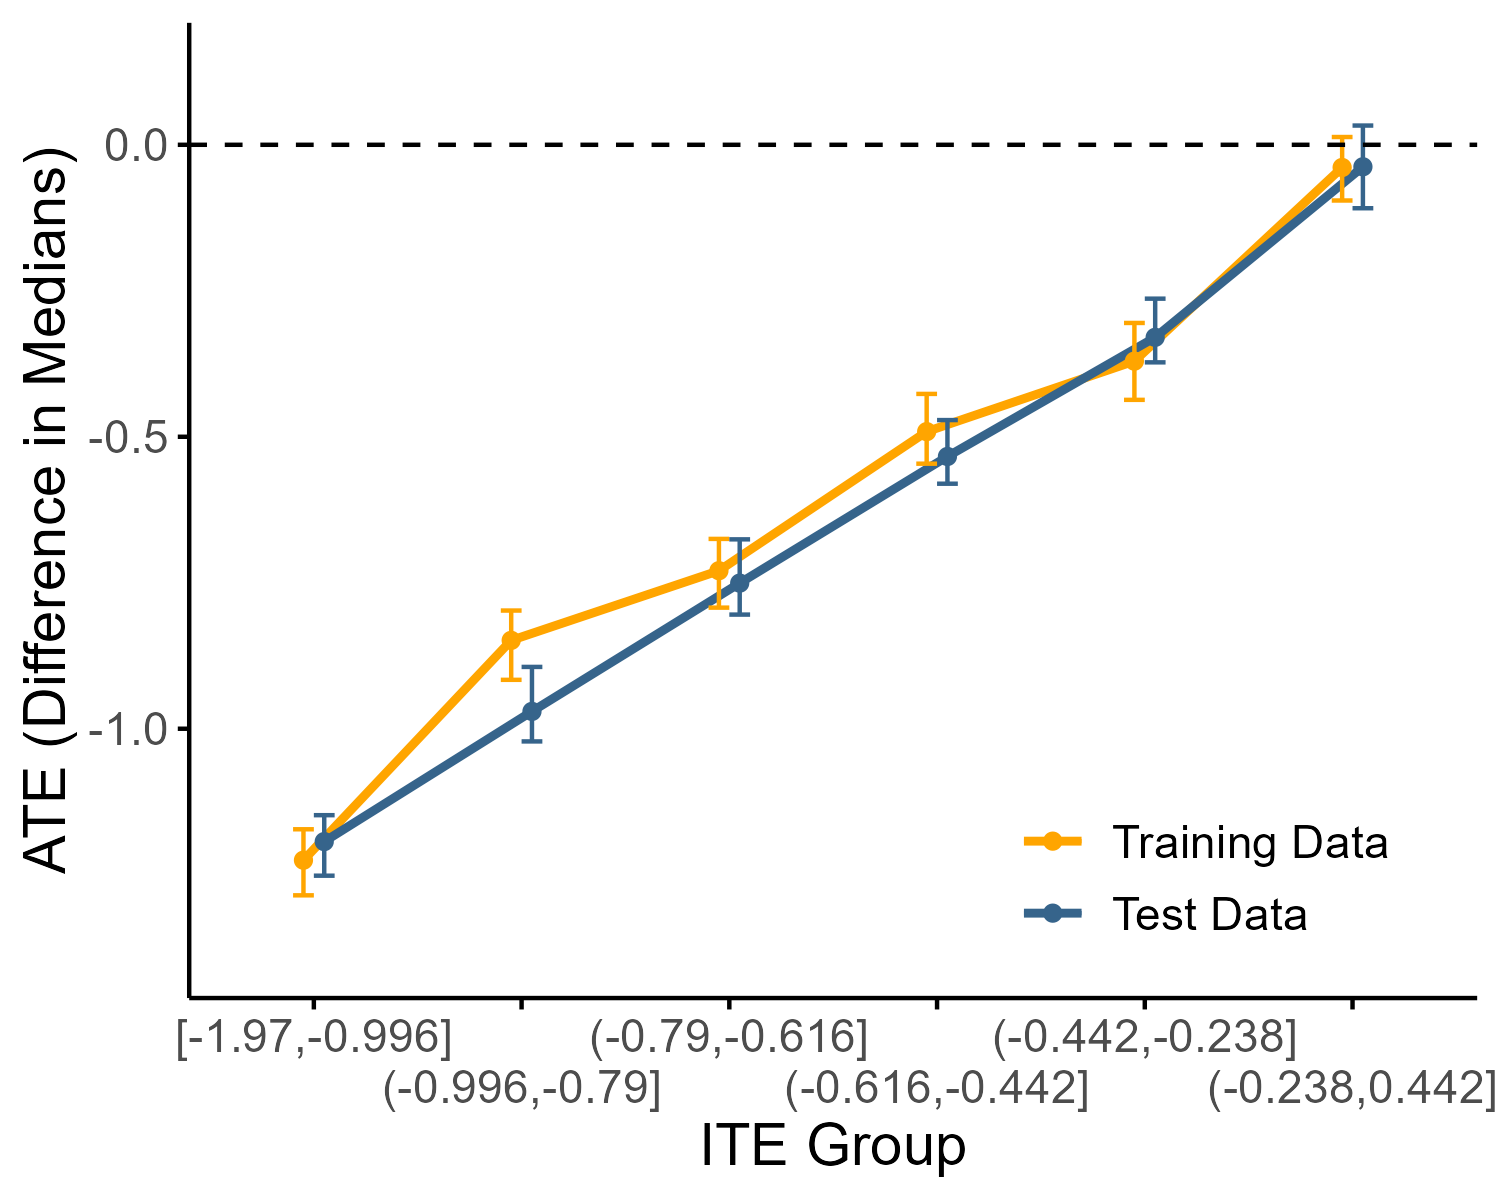
\includegraphics[width=0.45\textwidth]{img/results/rct_scenario1_ITE_cATE.png}
\caption{ITE-ATE plot for scenario (1), including direct and interaction effects. Individuals are grouped into bins according to the estimated ITE and in each bin the ATE is calculated as the difference in medians of the observed outcomes under the treatments. 95\% bootstrap confidence intervals indicate the uncertainty. Left: Observational; right: RCT setting.}
\label{fig:scenario1_ite_cATE}
\end{figure}



% start a new page
\clearpage


\subsection{Scenario (2): With direct but no interaction effects}

Scenario (2) included a direct effect of the treatment on the outcome and coefficients of the interaction effects are set to zero. This results in less heterogeneity of ITE compared to scenario (1) as shown in Figure \ref{fig:scenario2_ite_distribution_dgp}. The observational and interventional densities sampled by the fitted TRAM-DAG are aligned with the true densities according to the DGP as illustrated in Figures \ref{fig:scenario2_sampling_distributions_vertical} and \ref{fig:scenario2_outcome_distributions}. A notable discrepancy in variance exists between the estimated and true ITEs, as illustrated in Figures \ref{fig:scenario2_ite_densities_train_test} and \ref{fig:scenario2_ite_scatter_train_test}. The ITE-ATE plot in Figure \ref{fig:scenario2_ite_cATE} shows a less informative view compared to scenario (1). Table \ref{tab:scenario2_ate_comparison} presents the ATE measures for scenario (2). In the test set of the RCT setting, the ATE in terms of the difference in medians of the observed outcomes was $-0.639$. In contrast, the ATE based on the estimated ITEs in the same dataset was $-0.586$.


\begin{table}[htbp]
\centering
\small
\caption{Scenario (2), including a direct treatment but no interaction effects: Comparison of ATE measures across train and test sets for the observational and RCT setting.}
\label{tab:scenario2_ate_comparison}
\begin{tabular}{l c c c c}
\toprule
\textbf{Measure} & \multicolumn{2}{c}{\textbf{Observational}} & \multicolumn{2}{c}{\textbf{RCT}} \\
\cmidrule(lr){2-3} \cmidrule(lr){4-5}
 & \textbf{Train} & \textbf{Test} & \textbf{Train} & \textbf{Test} \\
\midrule
ATE as $\text{mean}(\text{Y}_\text{observed}^{(1)}) - \text{mean}(\text{Y}_\text{observed}^{(0)})$ & NA & NA & -0.569 & -0.572 \\
ATE as $\text{median}(\text{Y}_\text{observed}^{(1)}) - \text{median}(\text{Y}_\text{observed}^{(0)})$  & NA & NA & -0.629 & -0.639 \\
ATE as mean(ITE$_\text{true}$)  & -0.633 & -0.633 & -0.633 & -0.633 \\
ATE as mean(ITE$_\text{estimated}$) & -0.645 & -0.644 & -0.587 & -0.586 \\
\bottomrule
\end{tabular}
\end{table}



\begin{figure}[htbp]
\centering
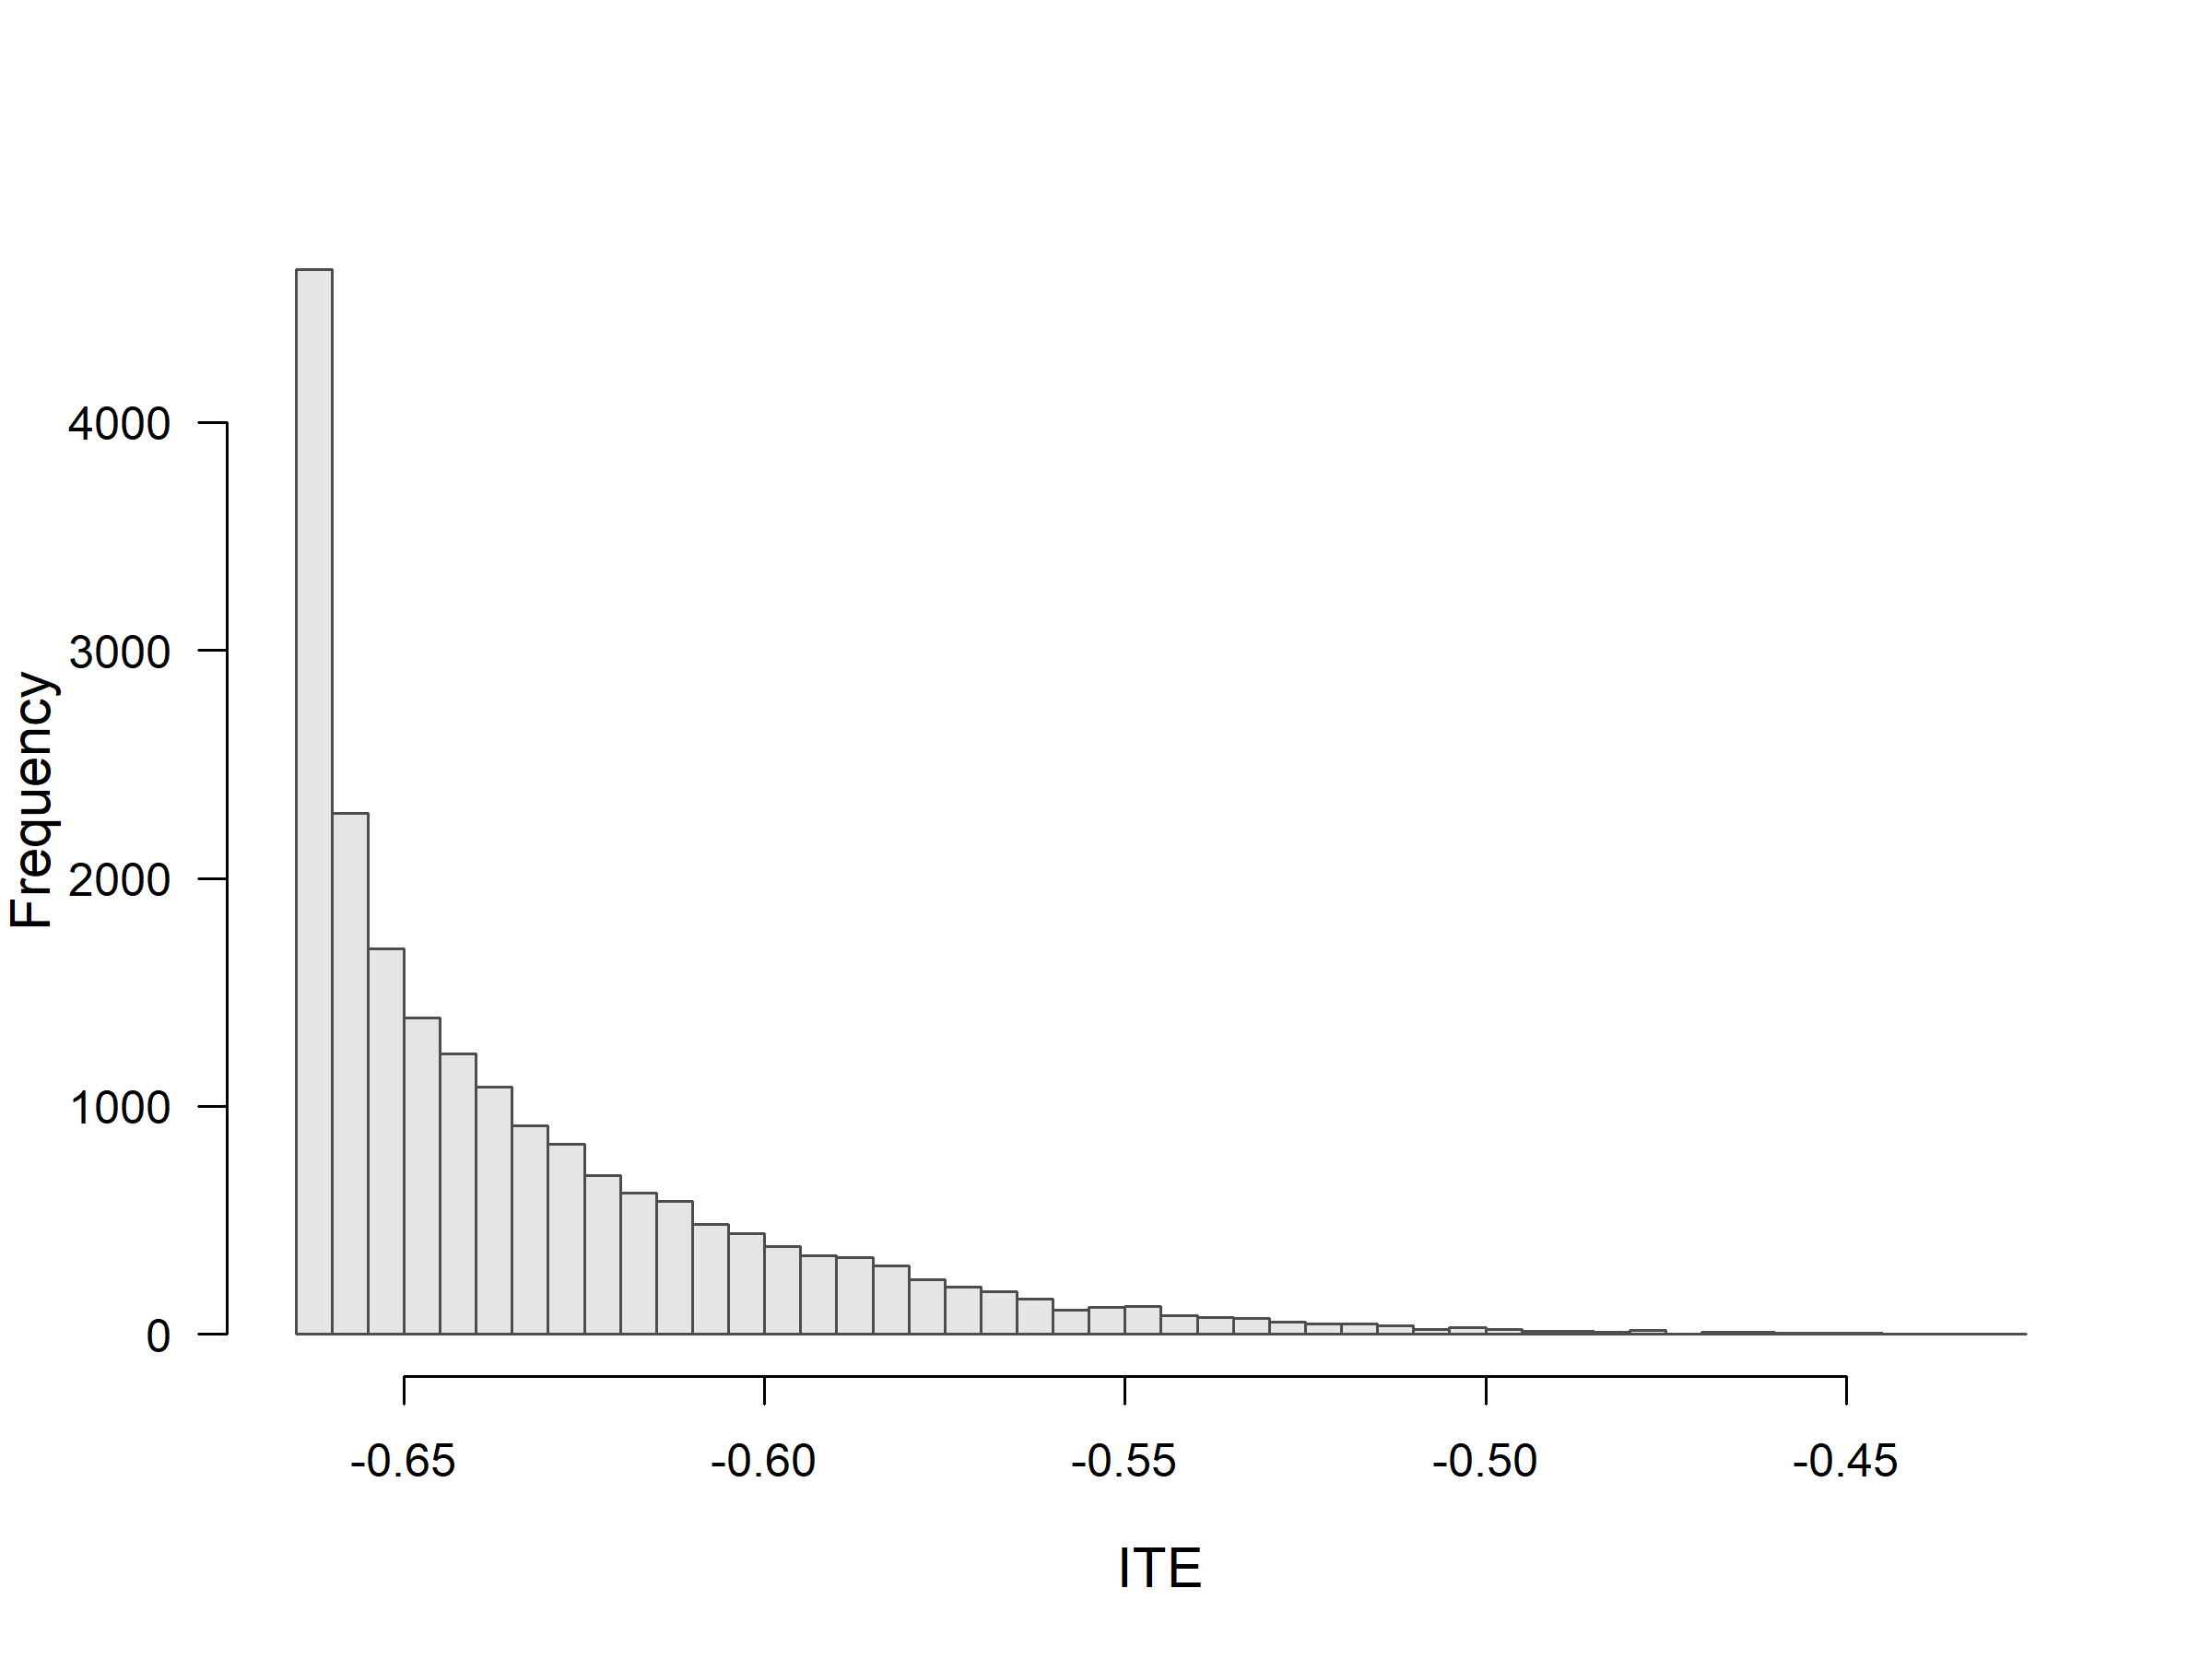
\includegraphics[width=0.45\textwidth]{img/results/observ_scenario2_ite_distribution_dgp.png}
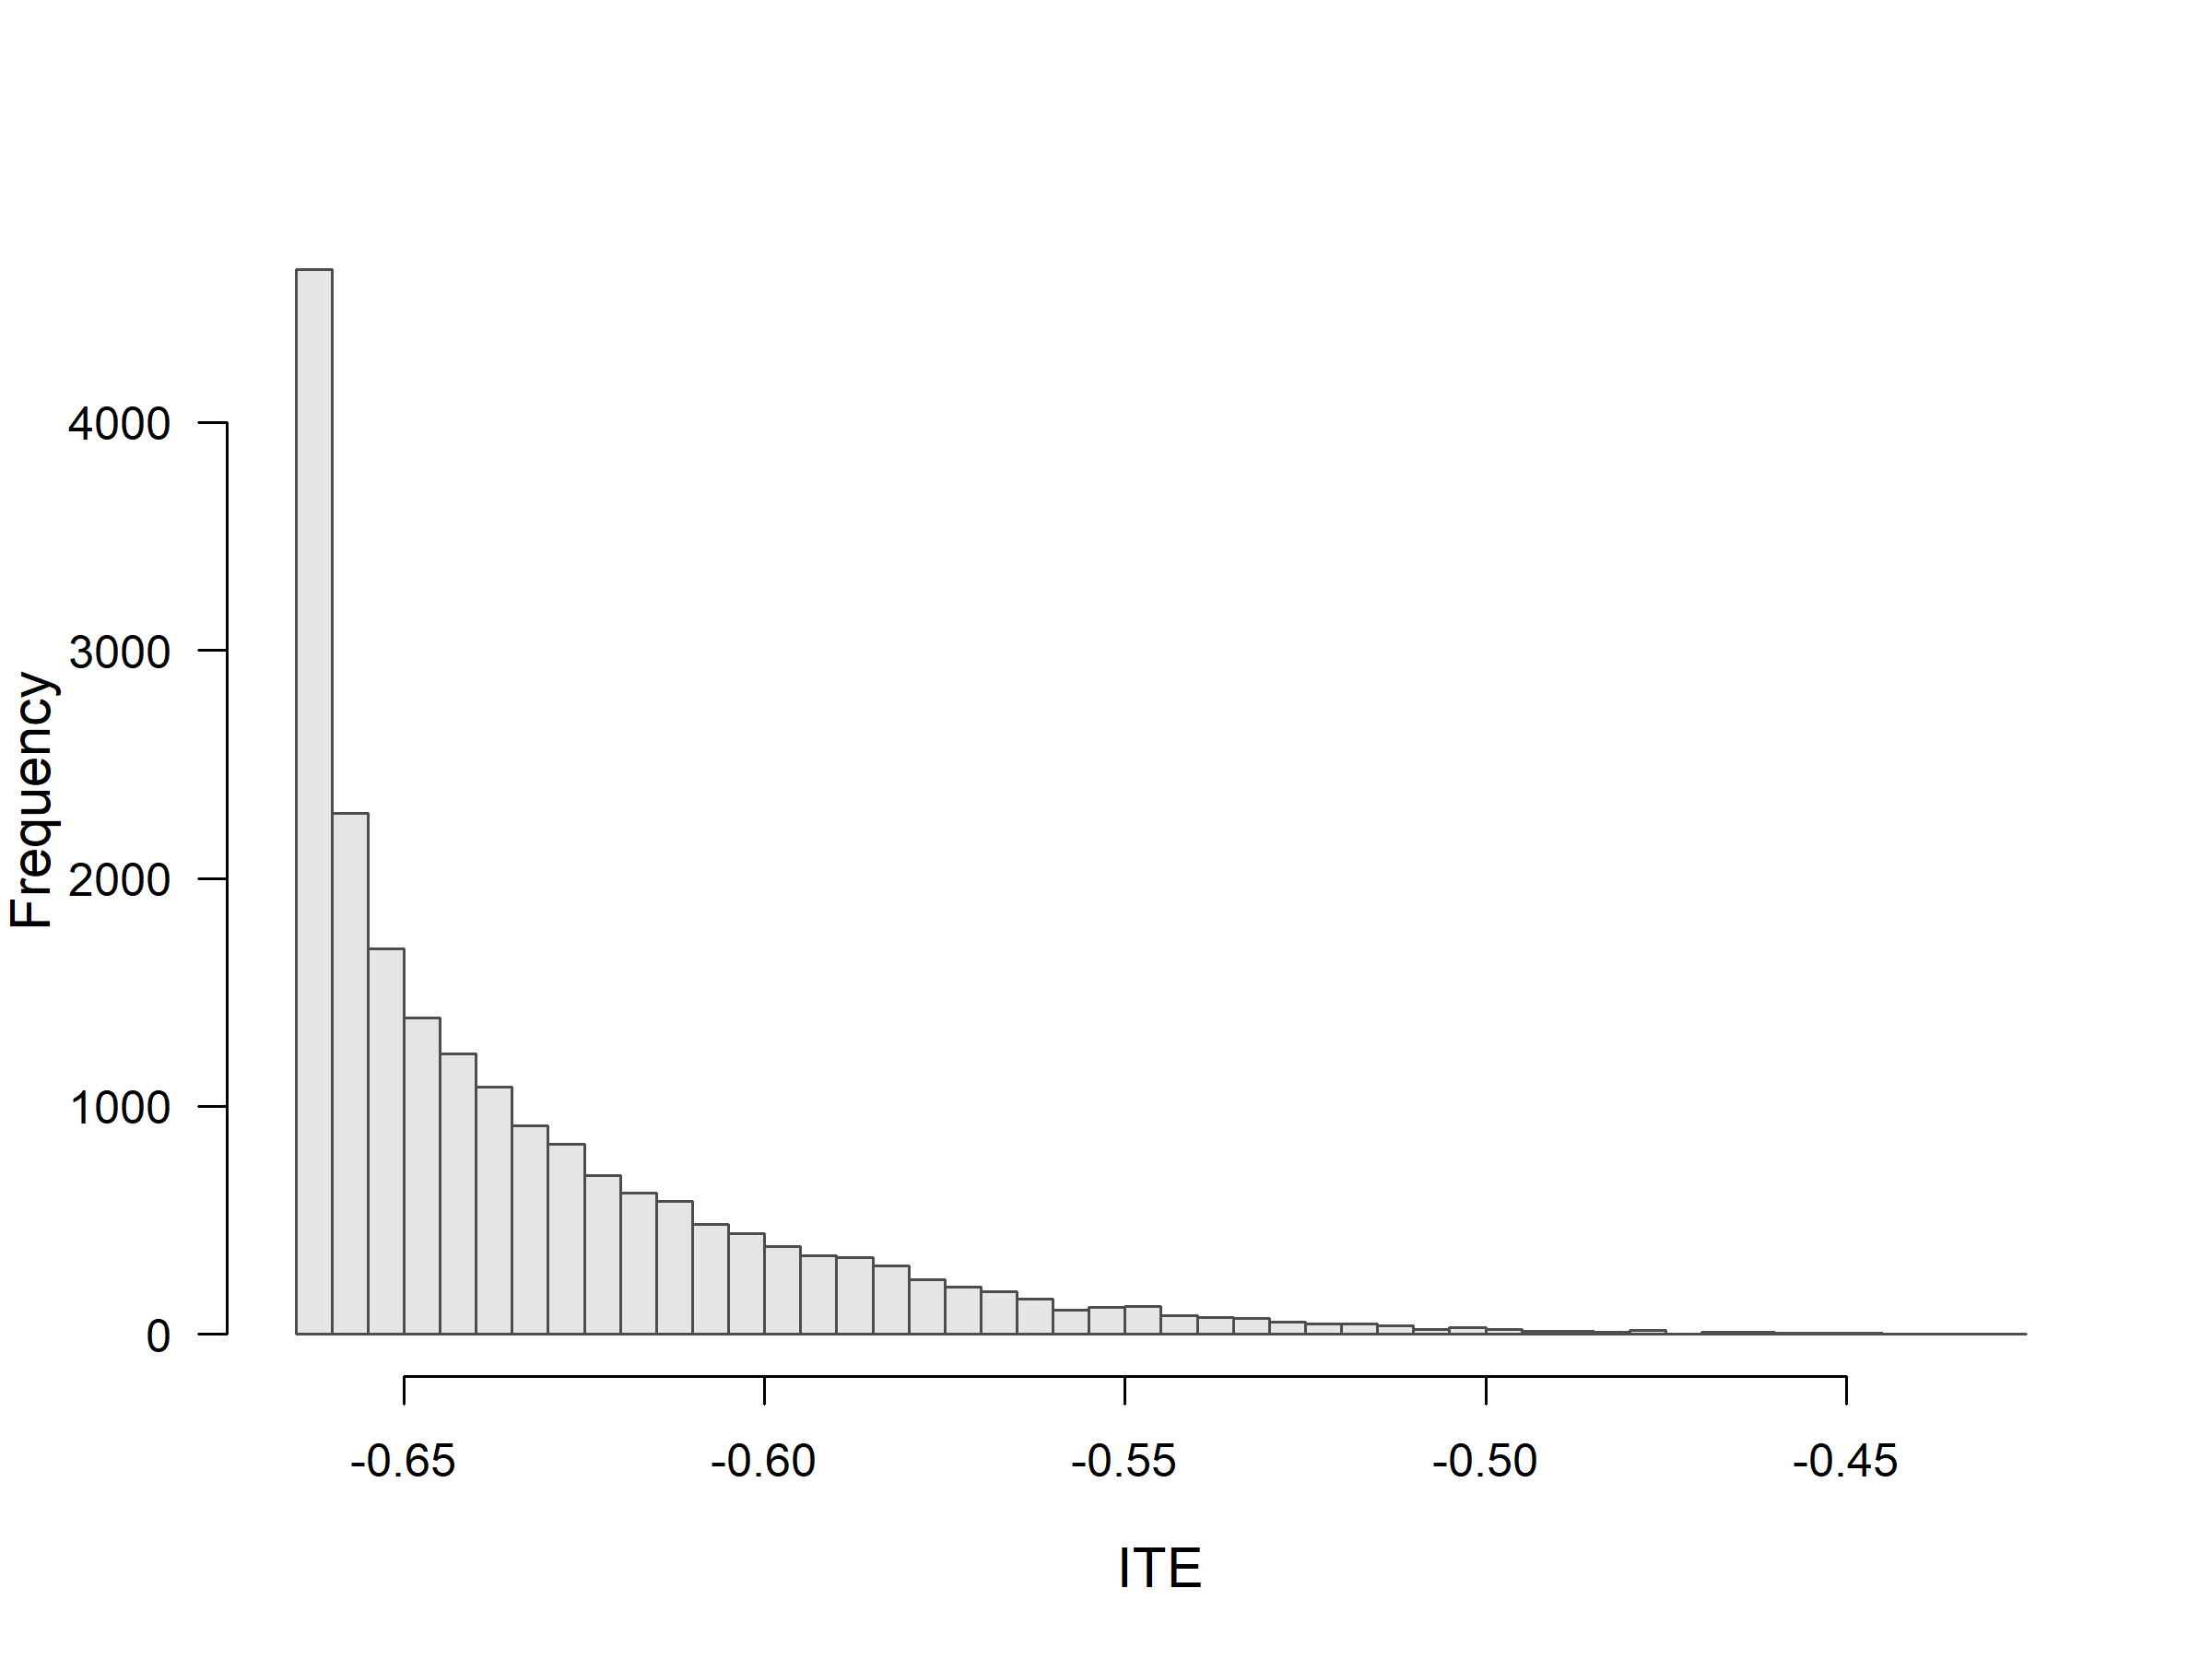
\includegraphics[width=0.45\textwidth]{img/results/rct_scenario2_ite_distribution_dgp.png}
\caption{True ITE distribution resulting from the DGP for scenario (2), including a direct treatment but no interaction effects. The true ITEs are identical in the observational and in the RCT setting, since they depend on the potential outcomes under both treatment allocations. Left: Observational; Right: RCT setting.}
\label{fig:scenario2_ite_distribution_dgp}
\end{figure}



\begin{figure}[htbp]
\centering
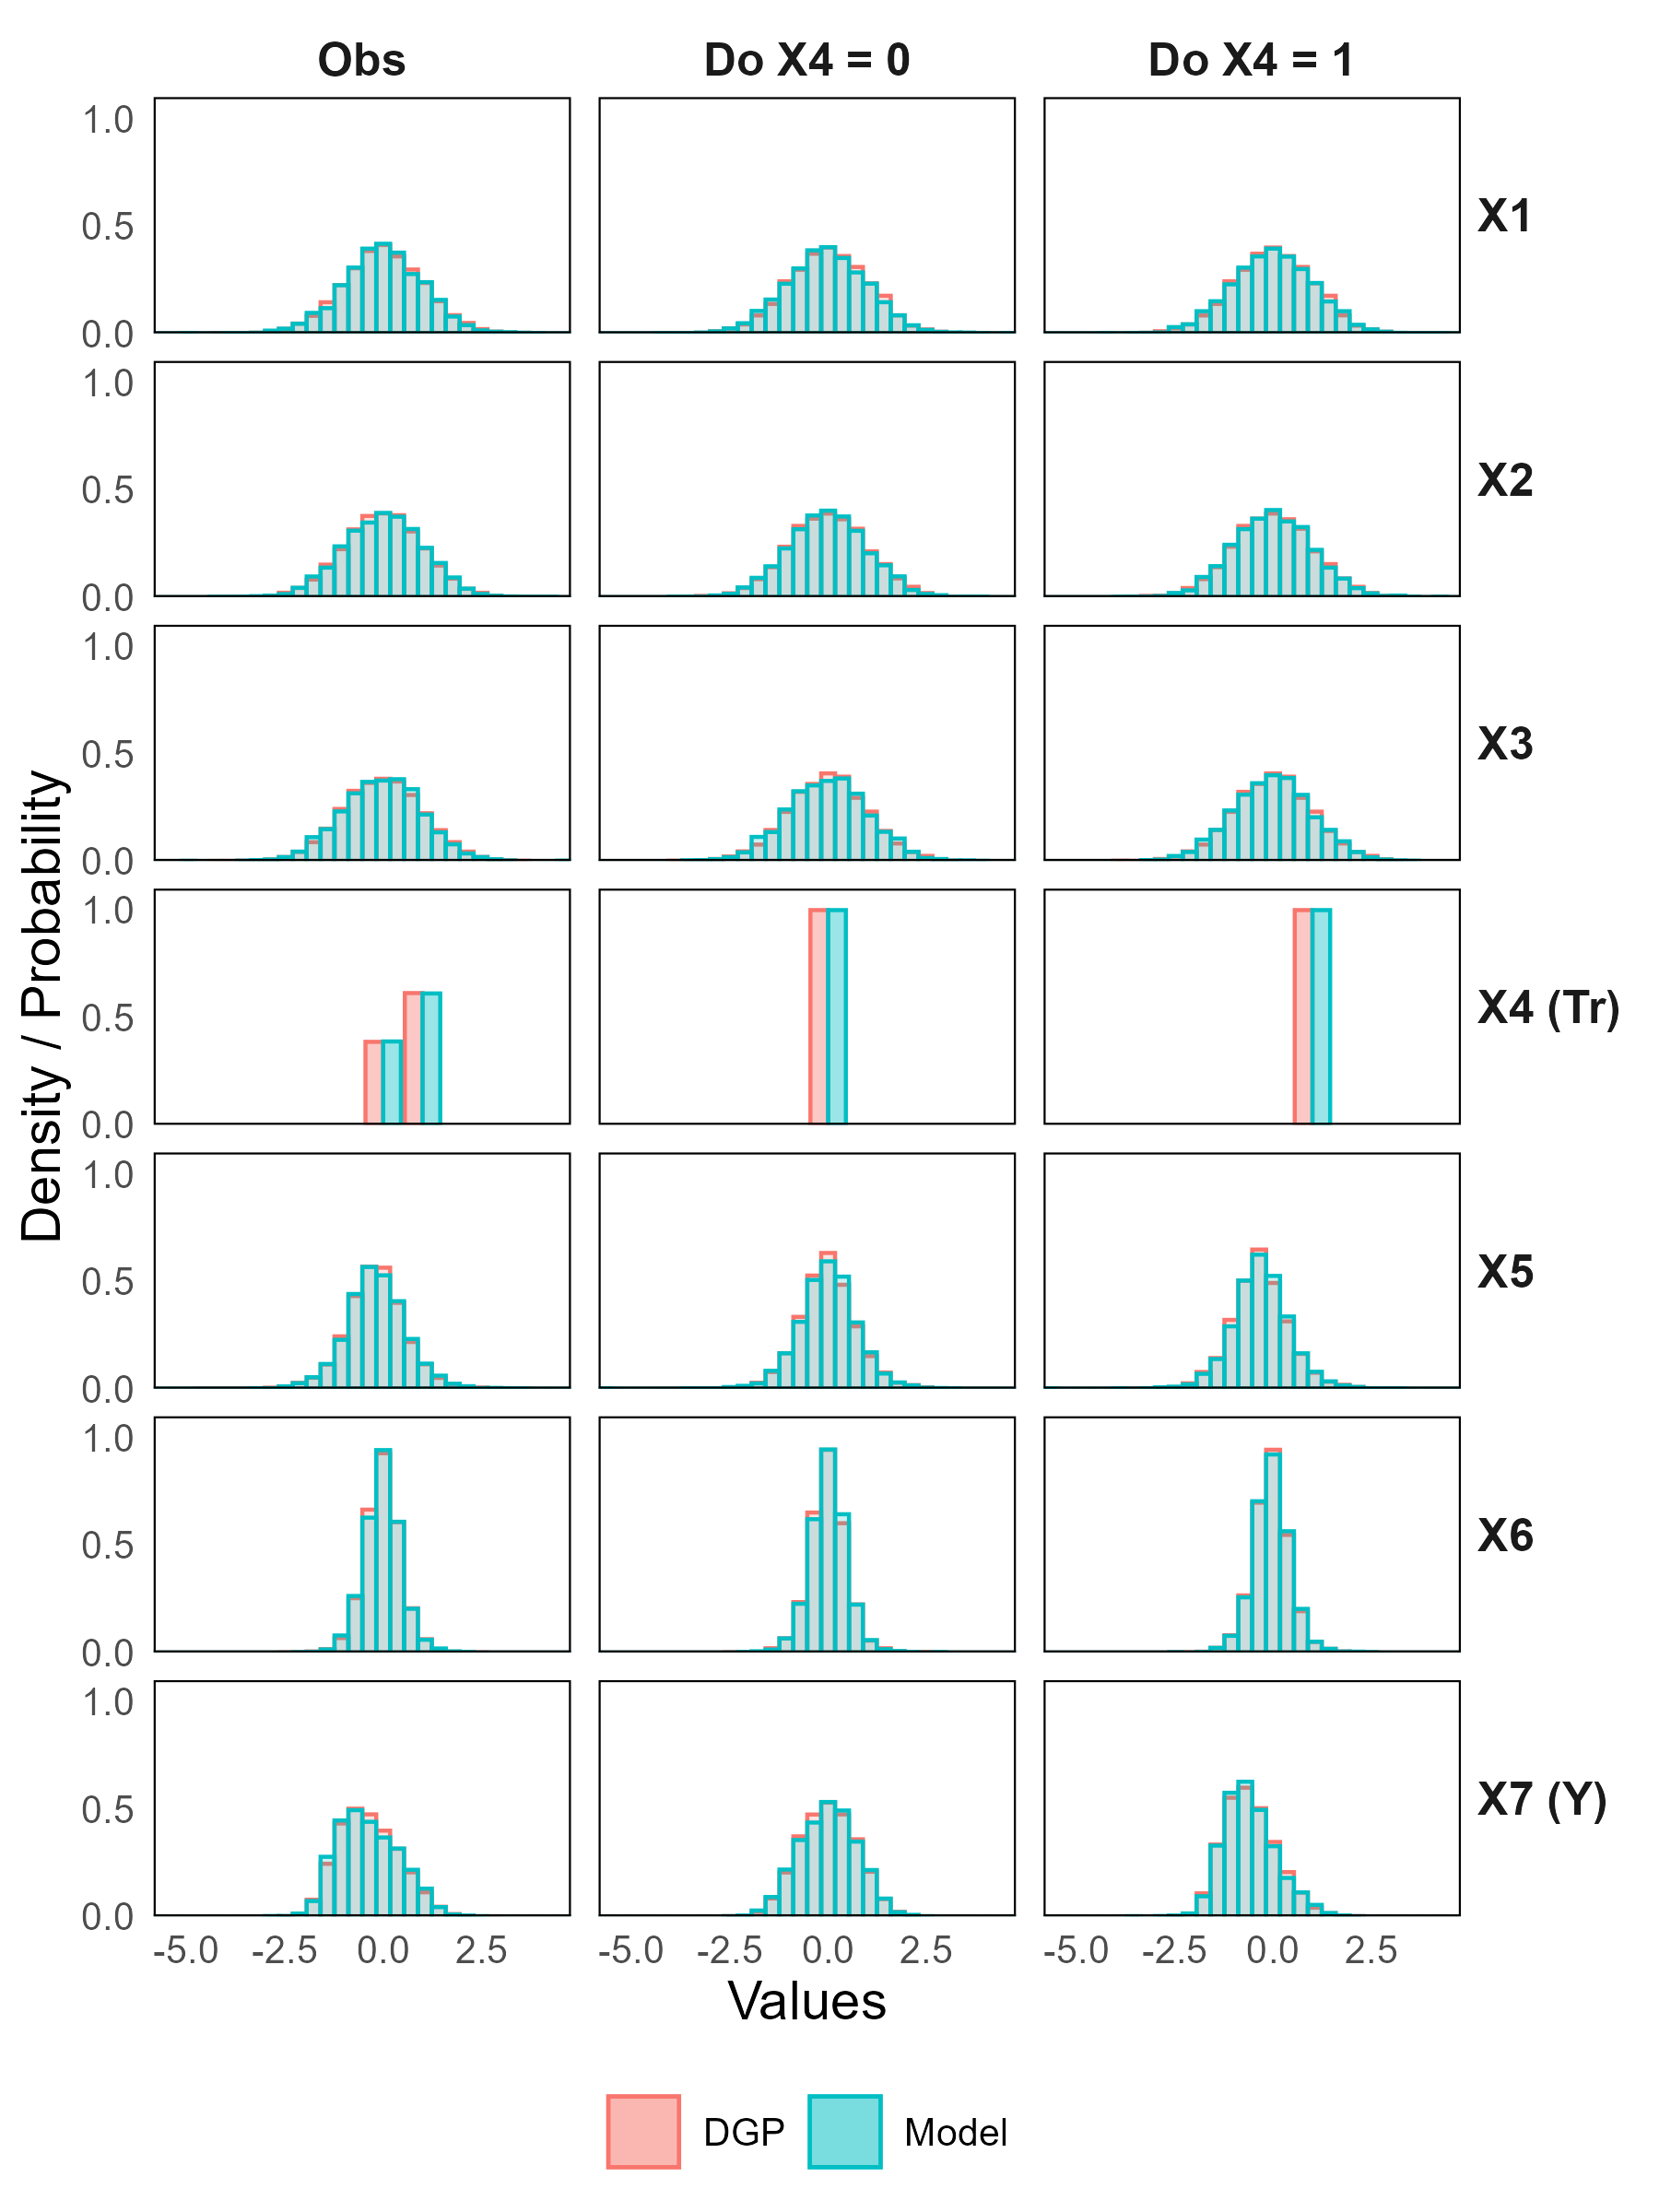
\includegraphics[width=0.45\textwidth]{img/results/observ_scenario2_sampling_distributions_vertical.png}
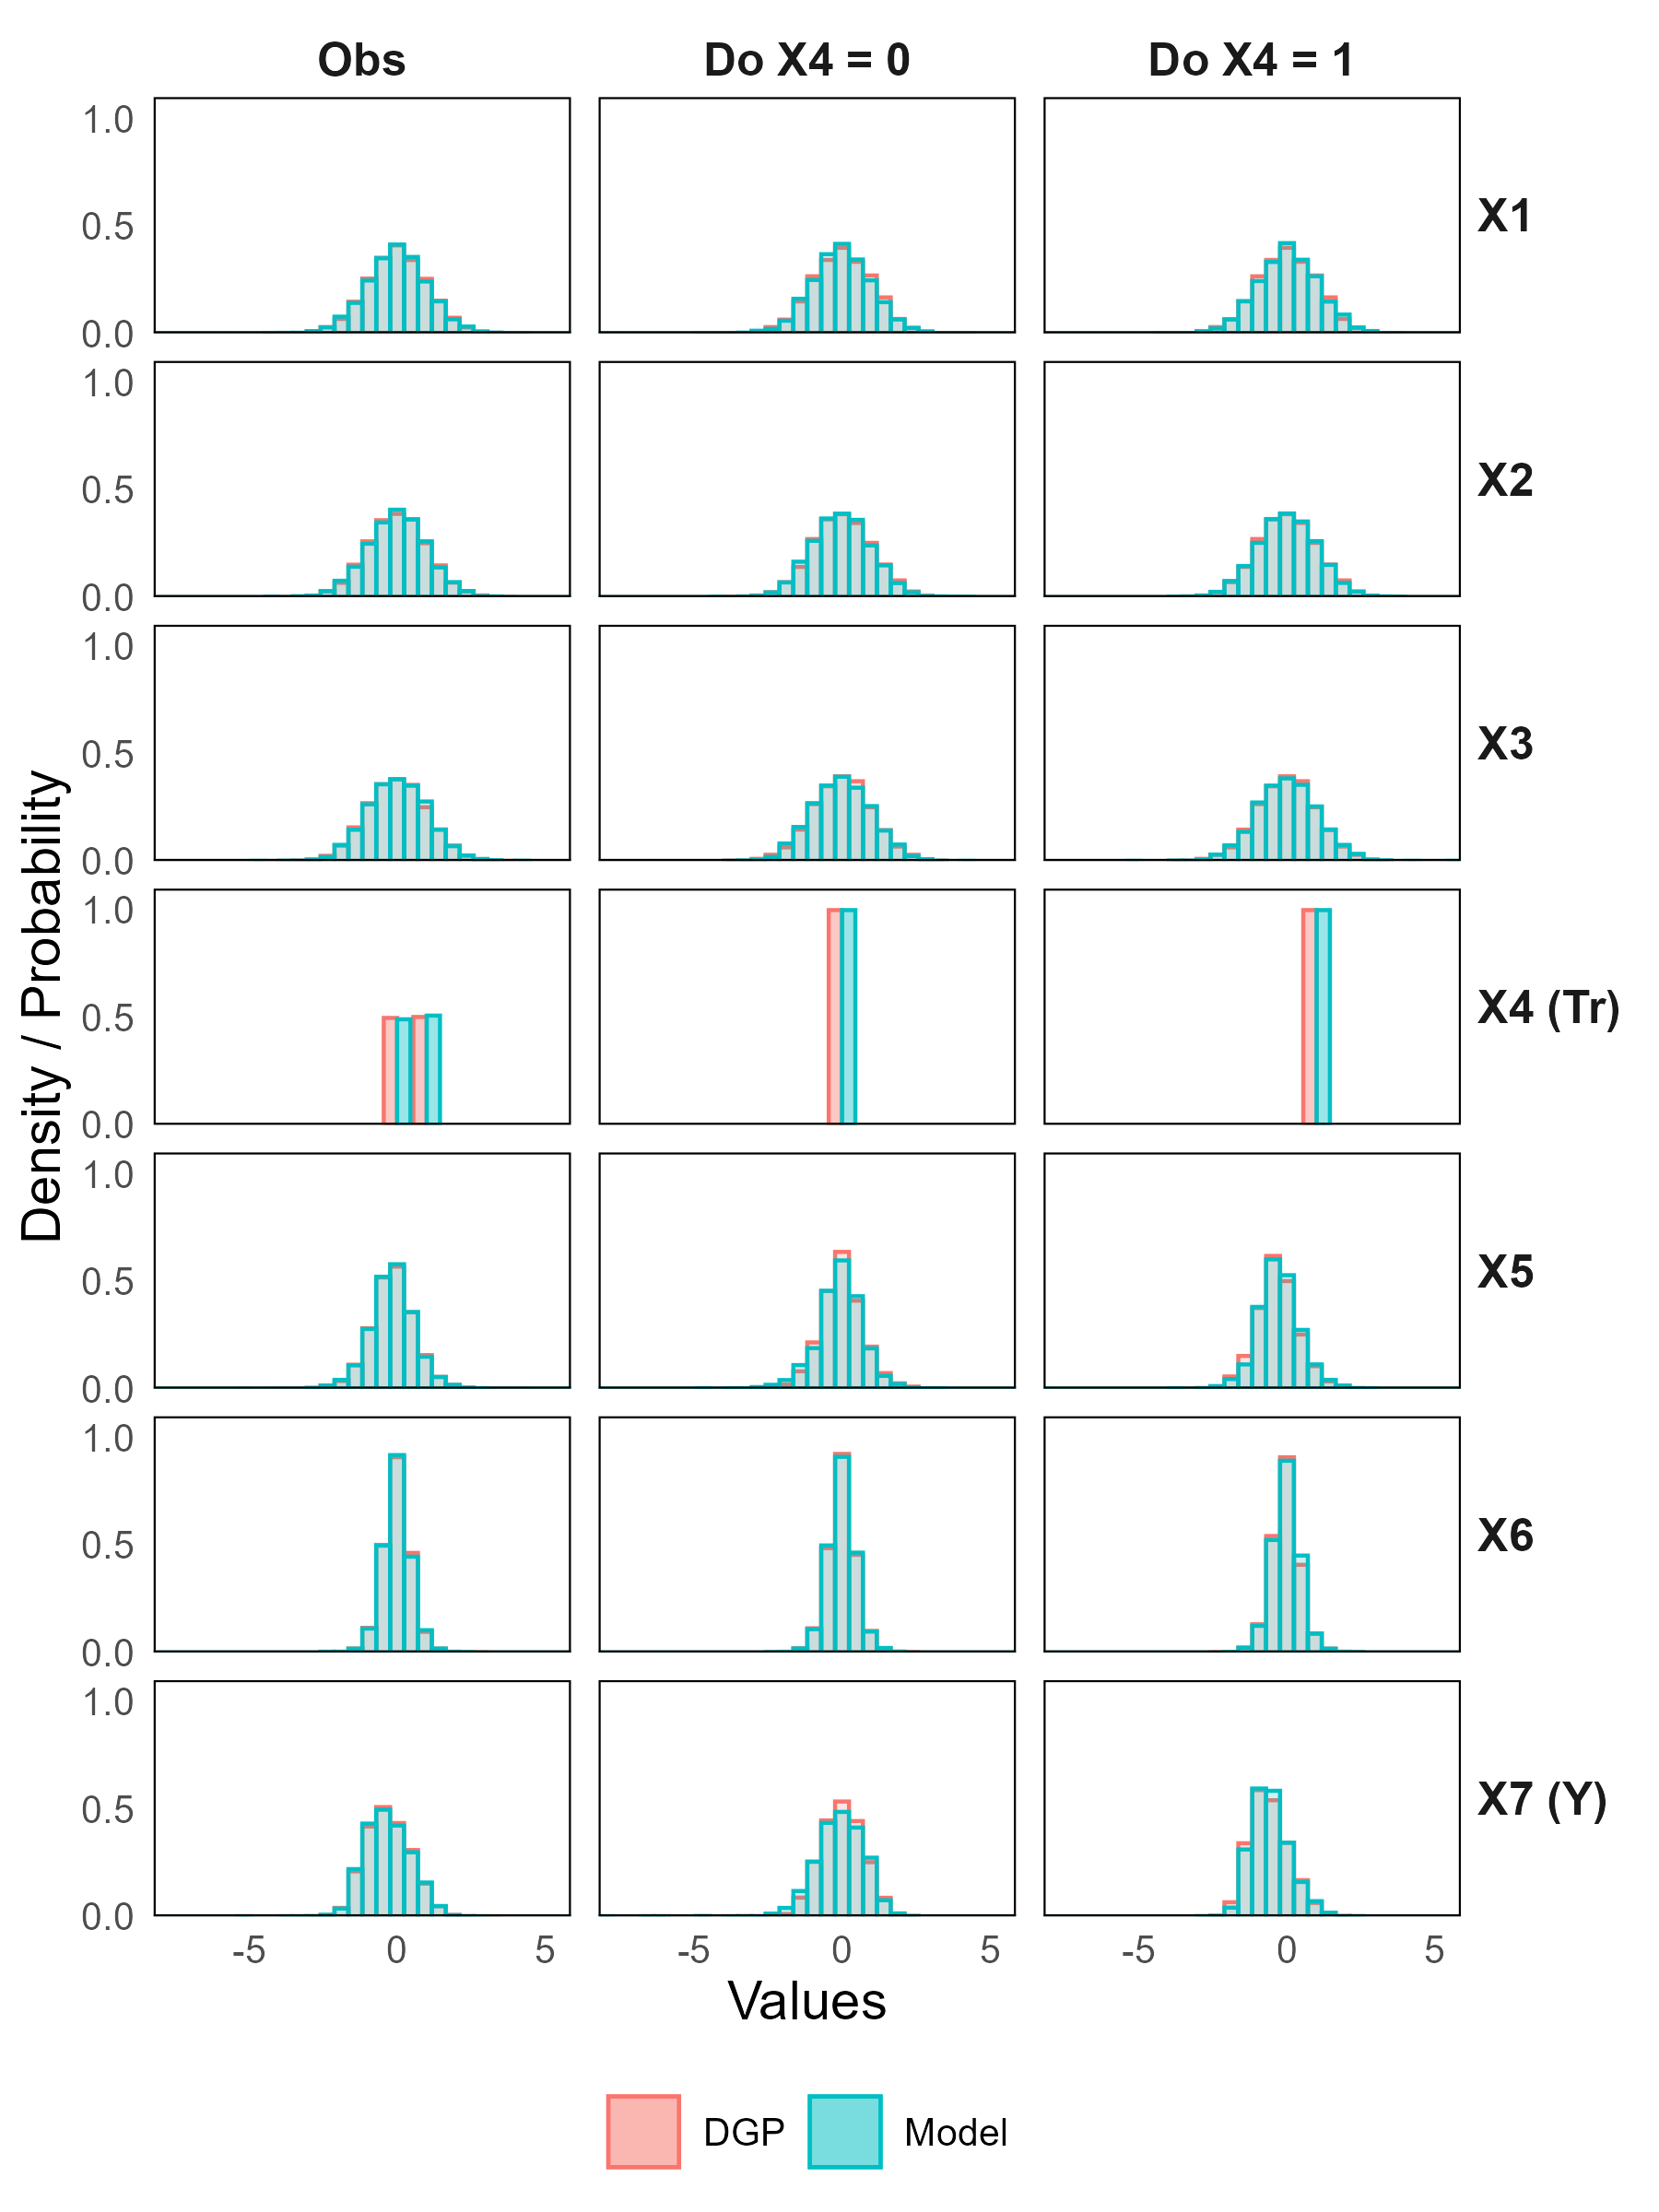
\includegraphics[width=0.45\textwidth]{img/results/rct_scenario2_sampling_distributions_vertical.png}
\caption{Marginal distributions of DGP variables and fitted TRAM-DAG samples for scenario (2), including a direct treatment but no interaction effects. The distributions shown as observed (Obs), under control intervention (Do $X4=0$) and under treatment intervention (Do $X4=1$). Left: Observational; Right: RCT setting.}
\label{fig:scenario2_sampling_distributions_vertical}
\end{figure}

\begin{figure}[htbp]
\centering
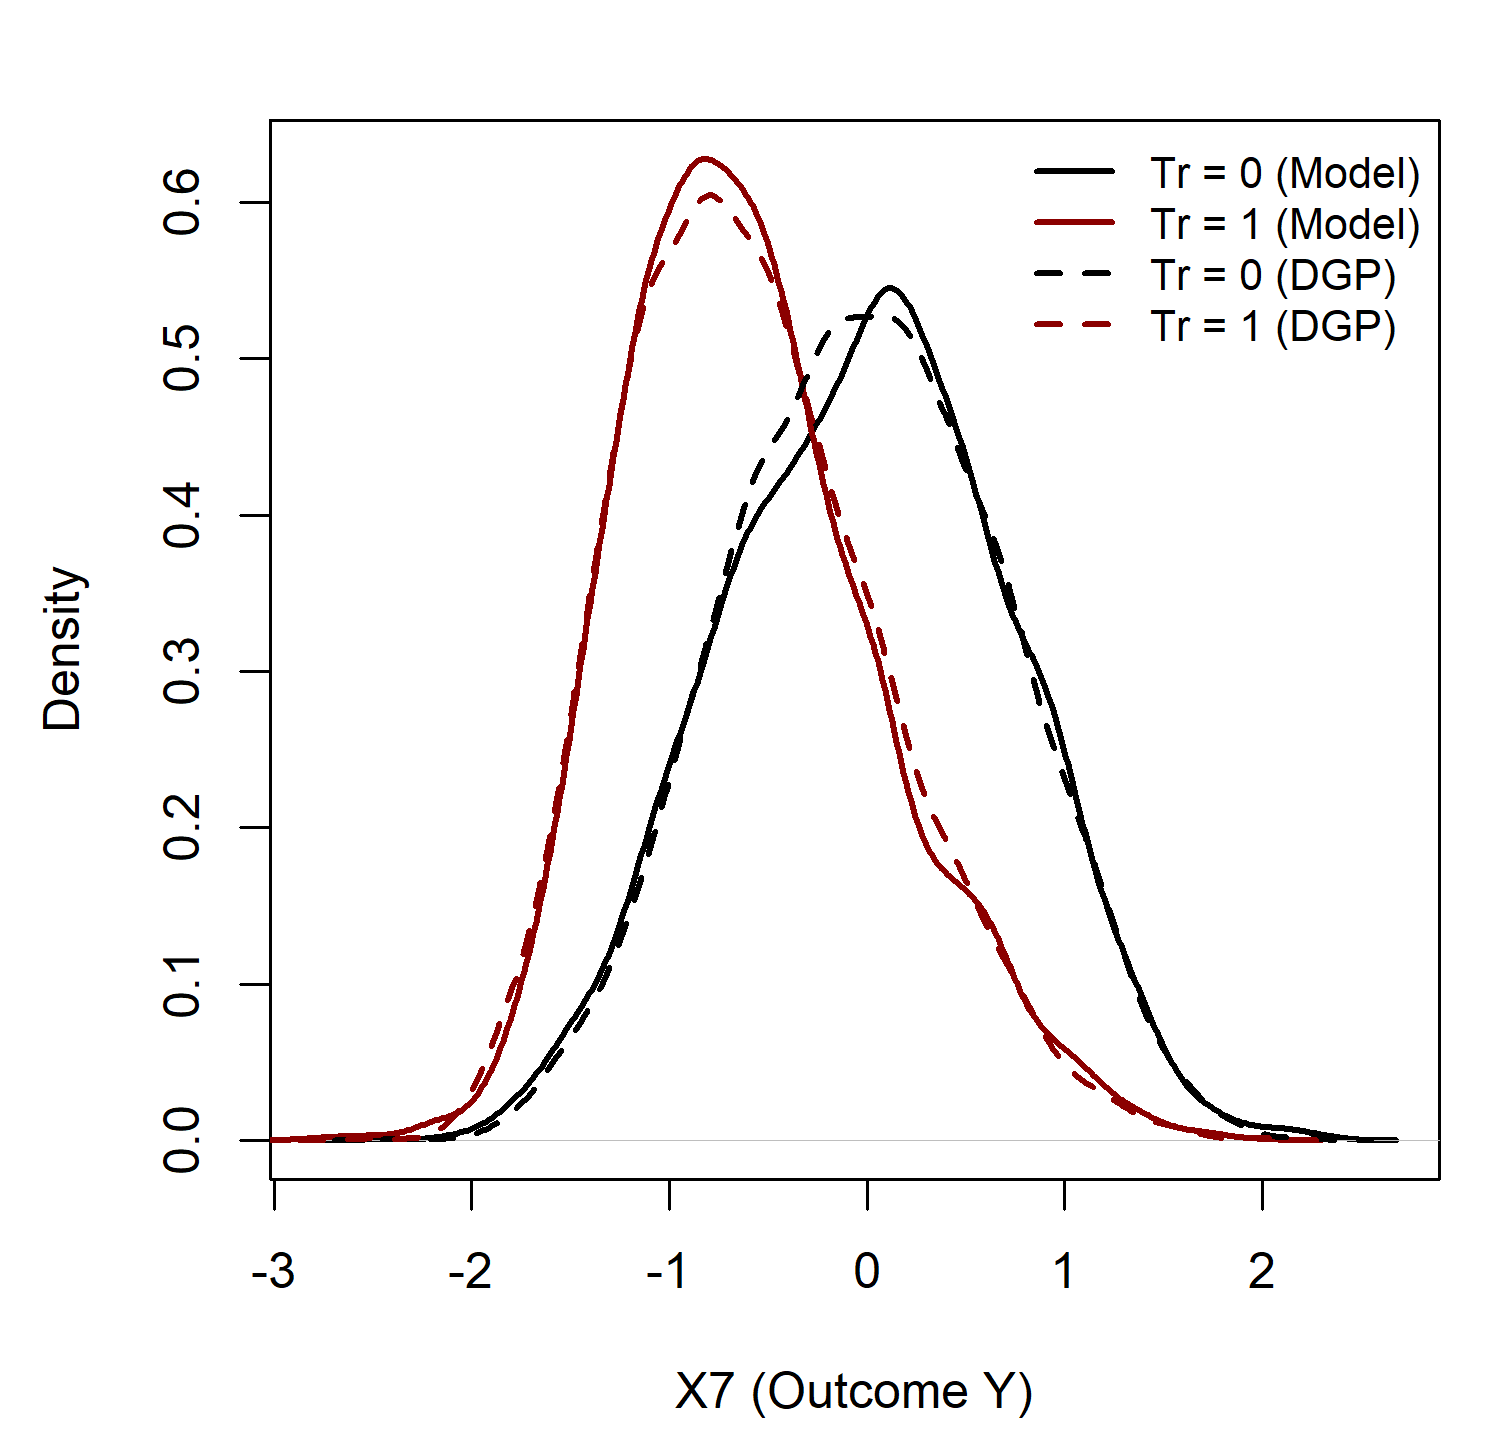
\includegraphics[width=0.45\textwidth]{img/results/observ_scenario2_X7_treatment_densities.png}
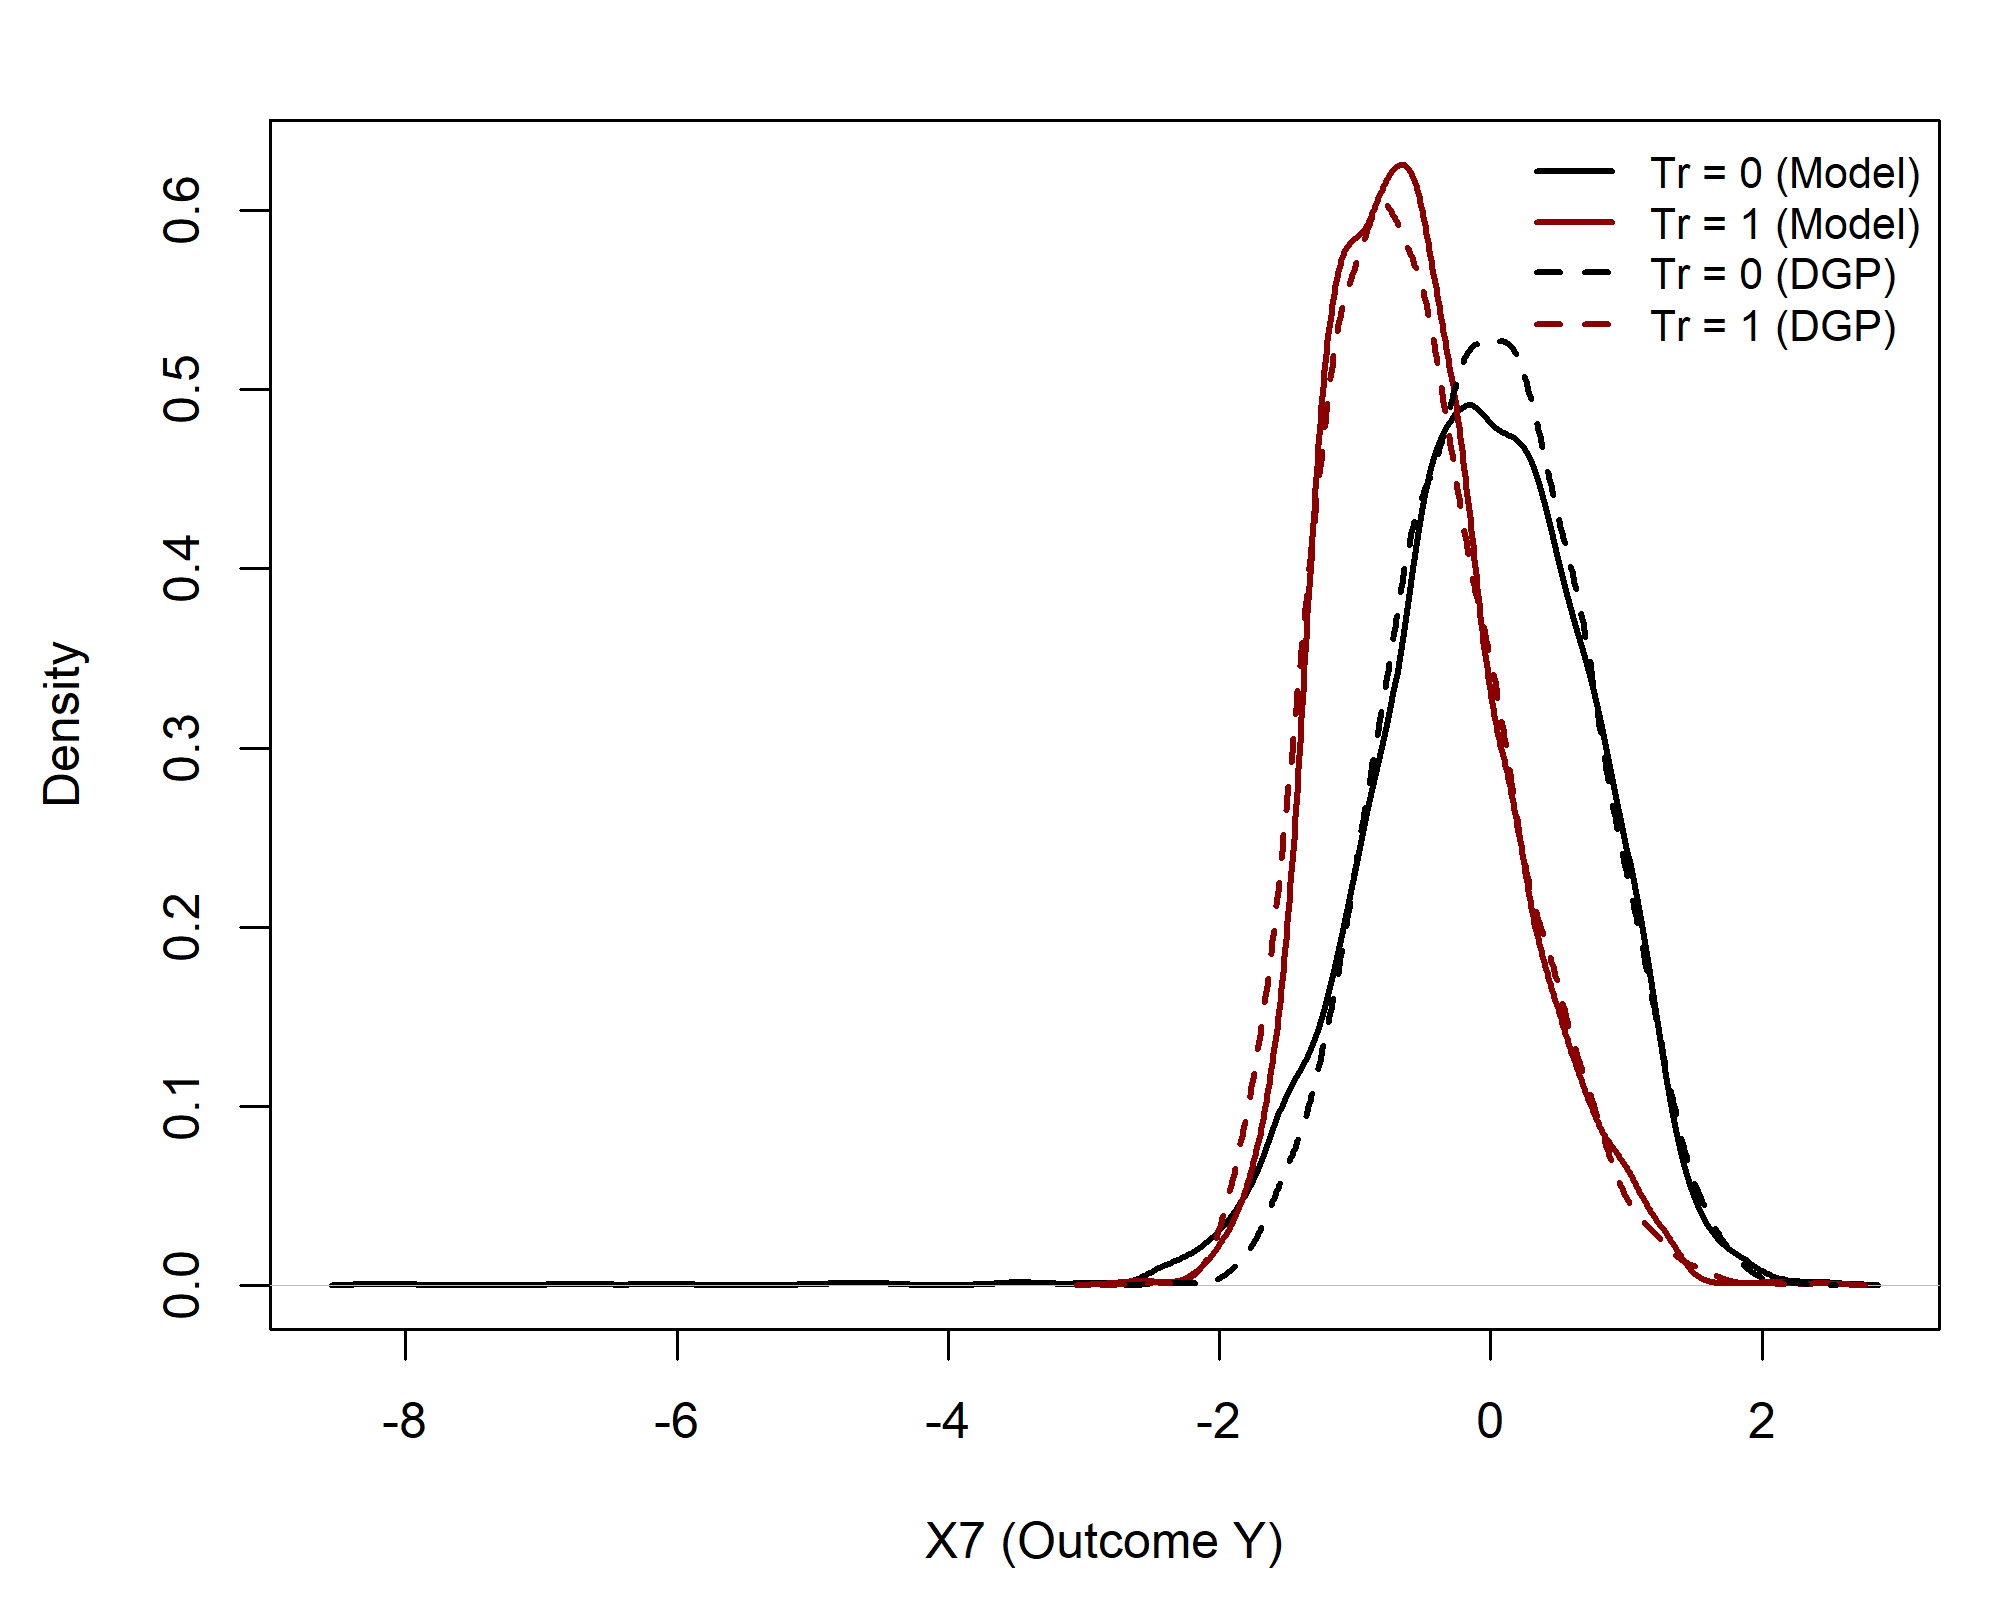
\includegraphics[width=0.45\textwidth]{img/results/rct_scenario2_X7_treatment_densities.png}
\caption{Distributions of the outcome variable (X7) under treatment and control interventions for scenario (2), including a direct treatment but no interaction effects. This plot is a higher resolution view of the X7 panels (Do $X4=0$) and (Do $X4=1$) from Figure \ref{fig:scenario2_sampling_distributions_vertical}. Left: Observational; Right: RCT setting.}
\label{fig:scenario2_outcome_distributions}
\end{figure}




\begin{figure}[htbp]
\centering
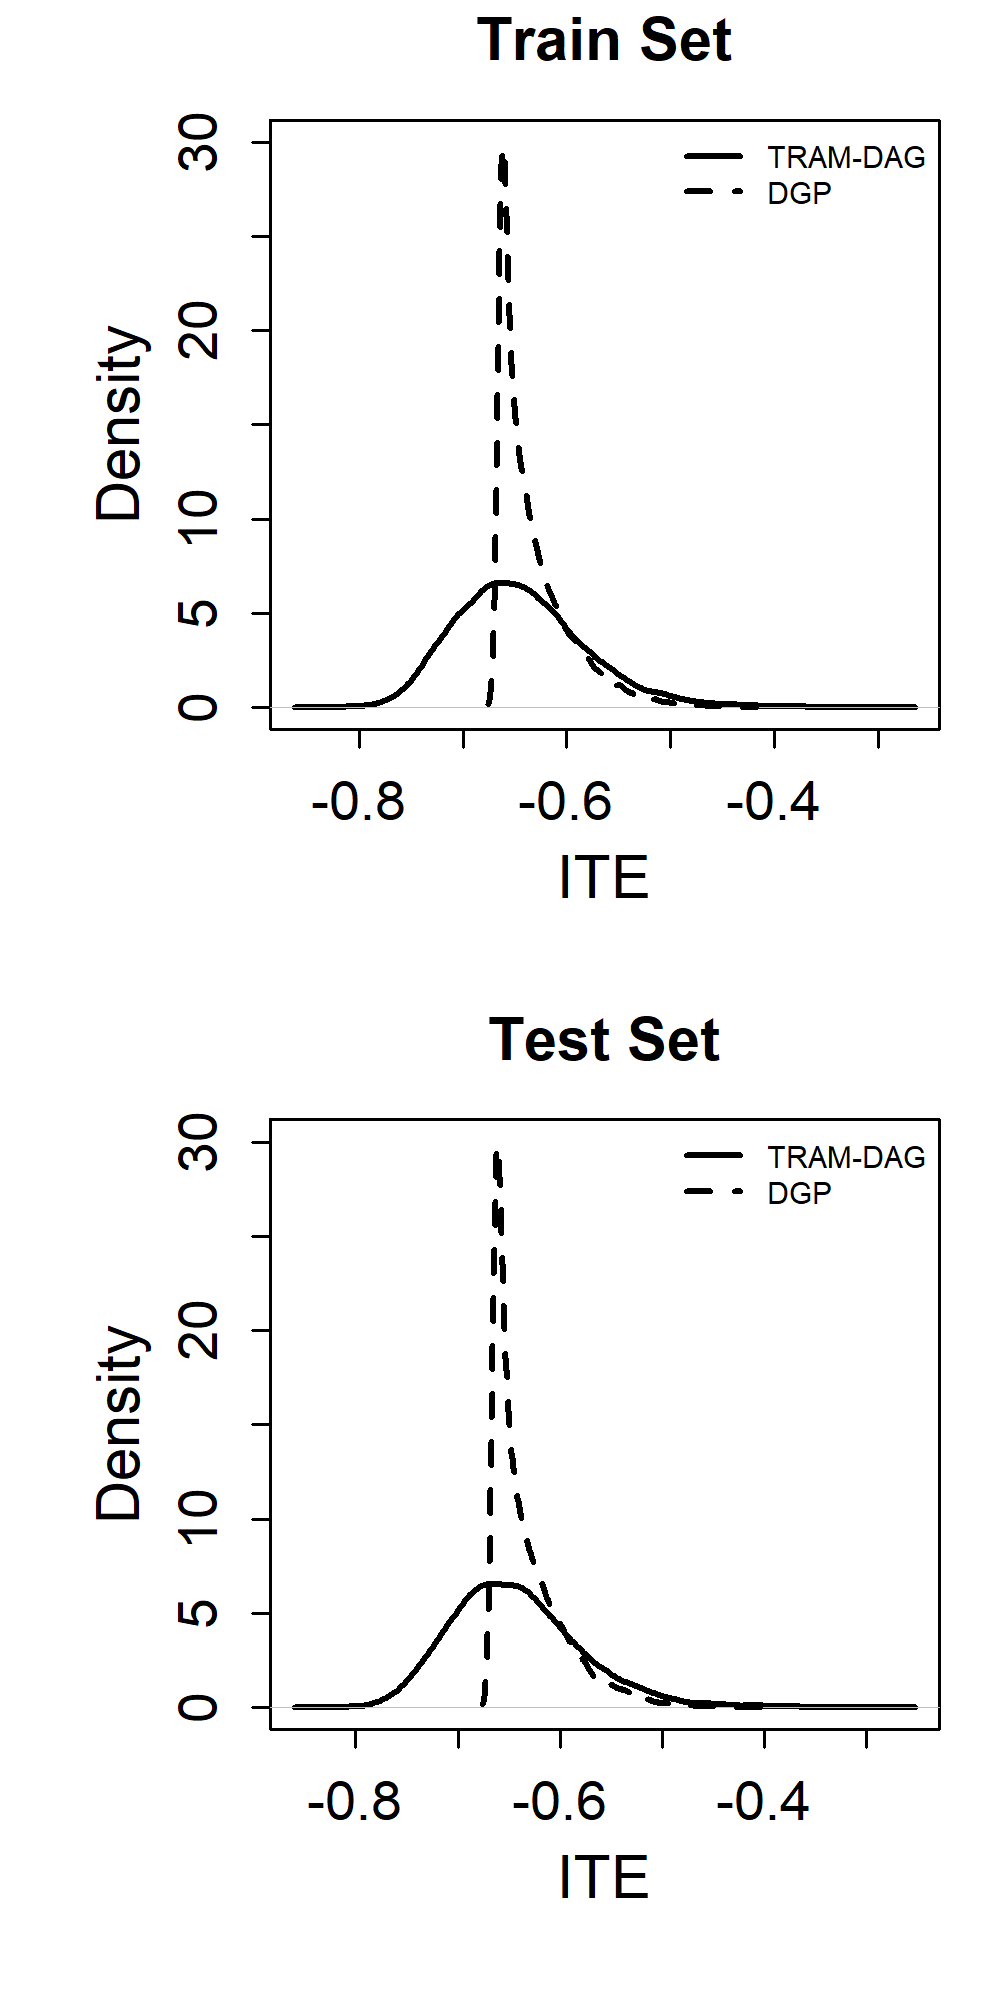
\includegraphics[width=0.45\textwidth]{img/results/observ_scenario2_ITE_densities_train_test.png}
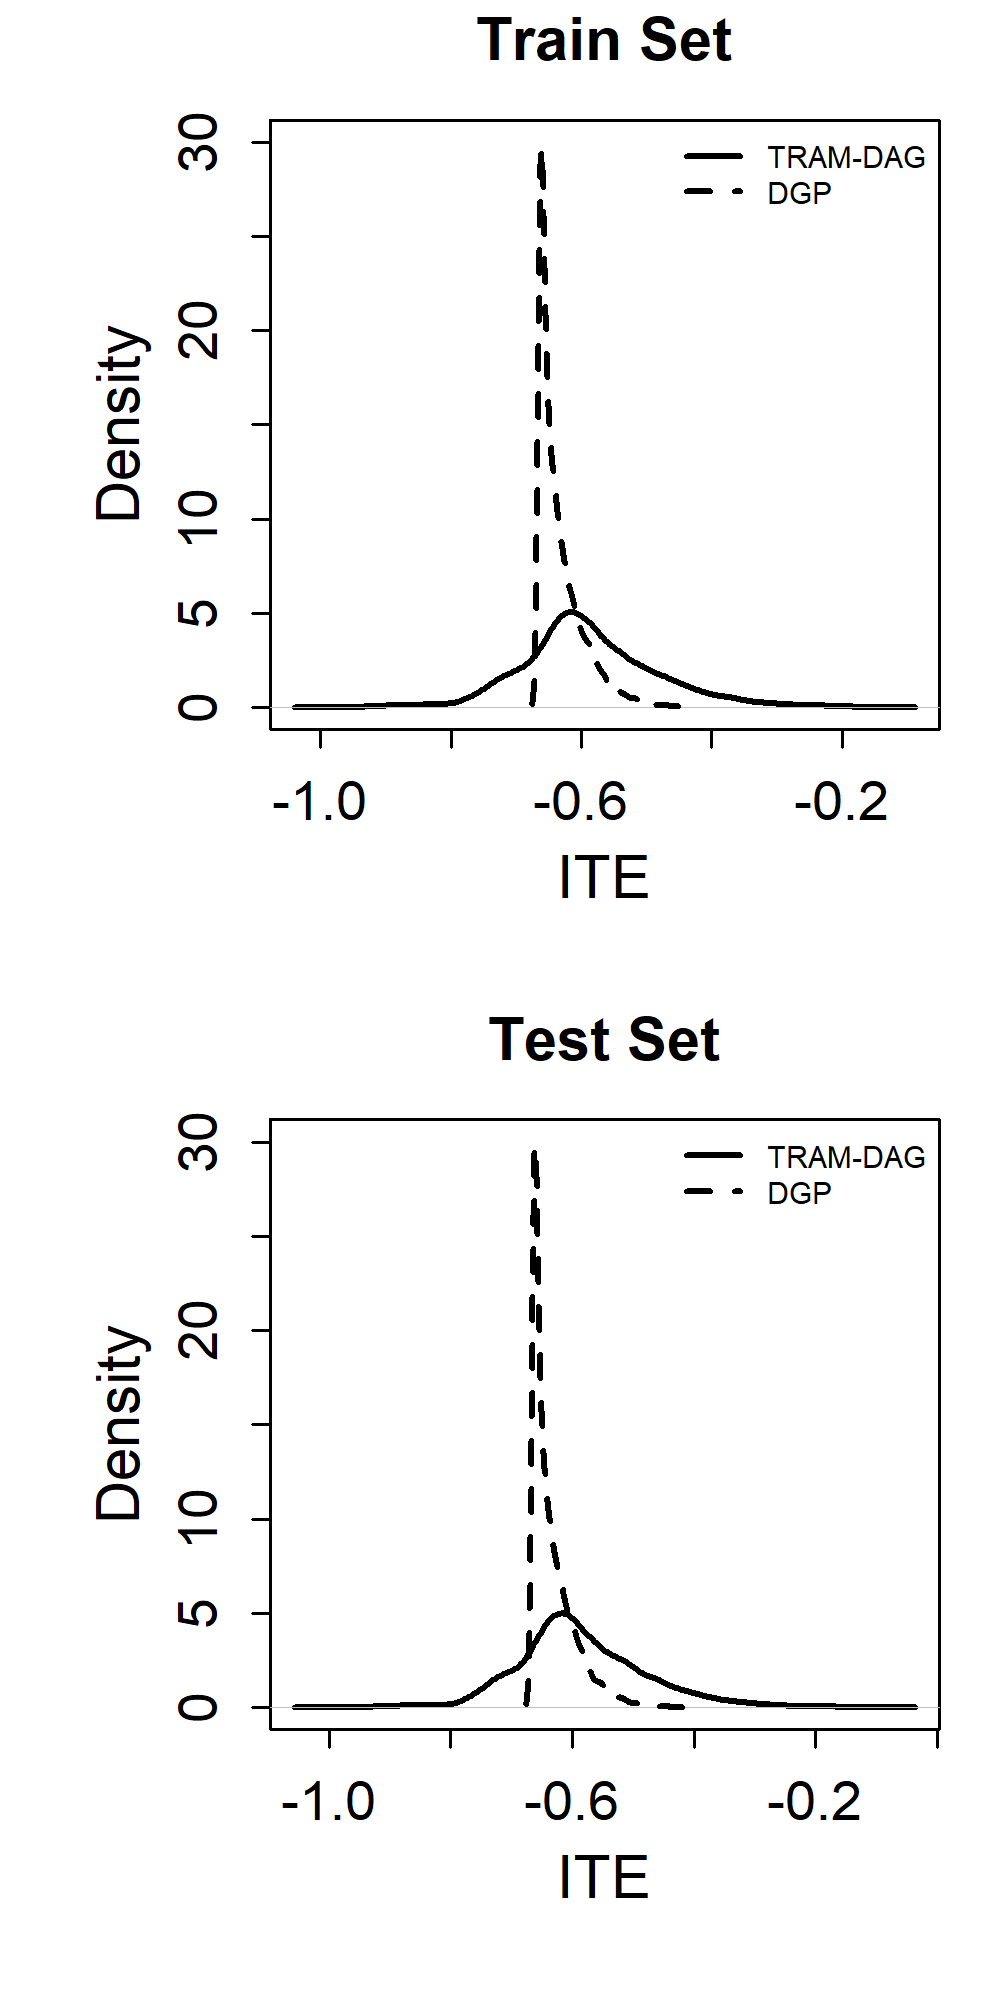
\includegraphics[width=0.45\textwidth]{img/results/rct_scenario2_ITE_densities_train_test.png}
\caption{Densities of estimated ITEs compared to the true ITEs in the training and test datasets for scenario (2), including a direct treatment but no interaction effects. Left: Observational; right: RCT setting.}
\label{fig:scenario2_ite_densities_train_test}
\end{figure}






\begin{figure}[htbp]
\centering
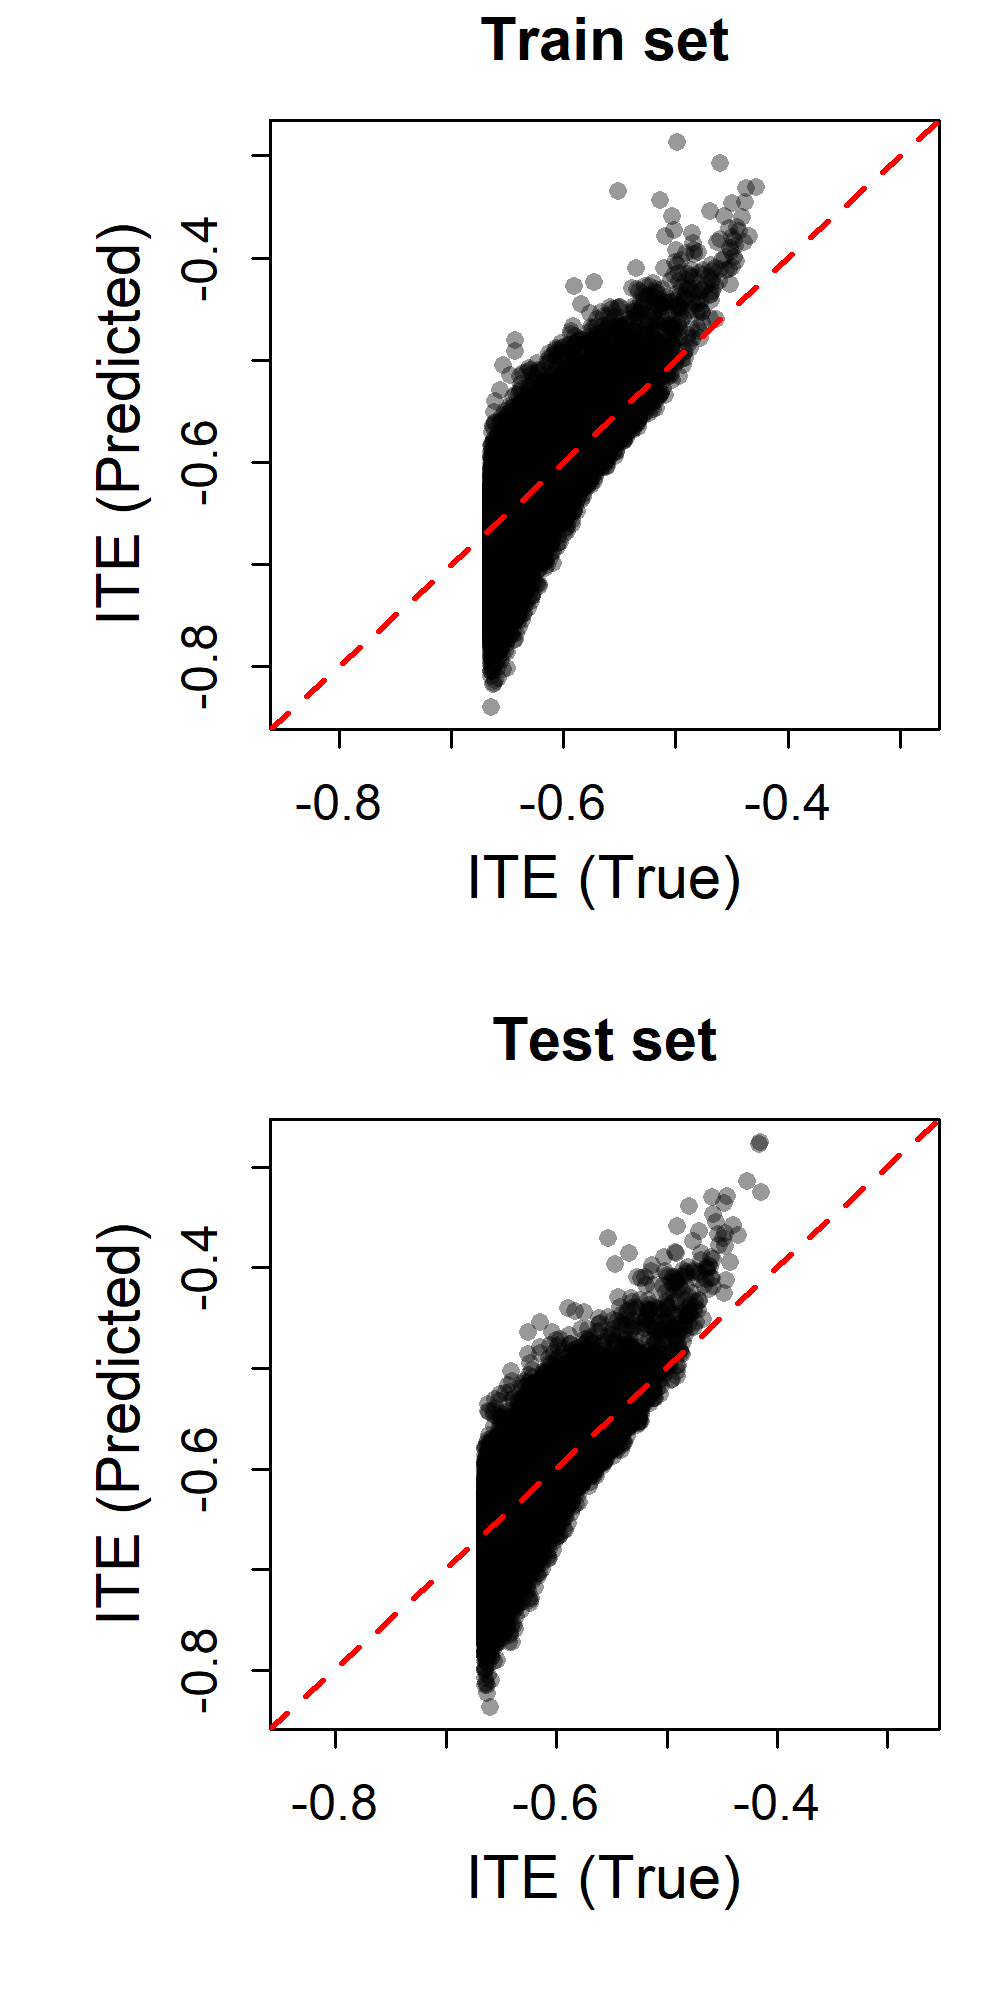
\includegraphics[width=0.45\textwidth]{img/results/observ_scenario2_ITE_scatter_train_test.png}
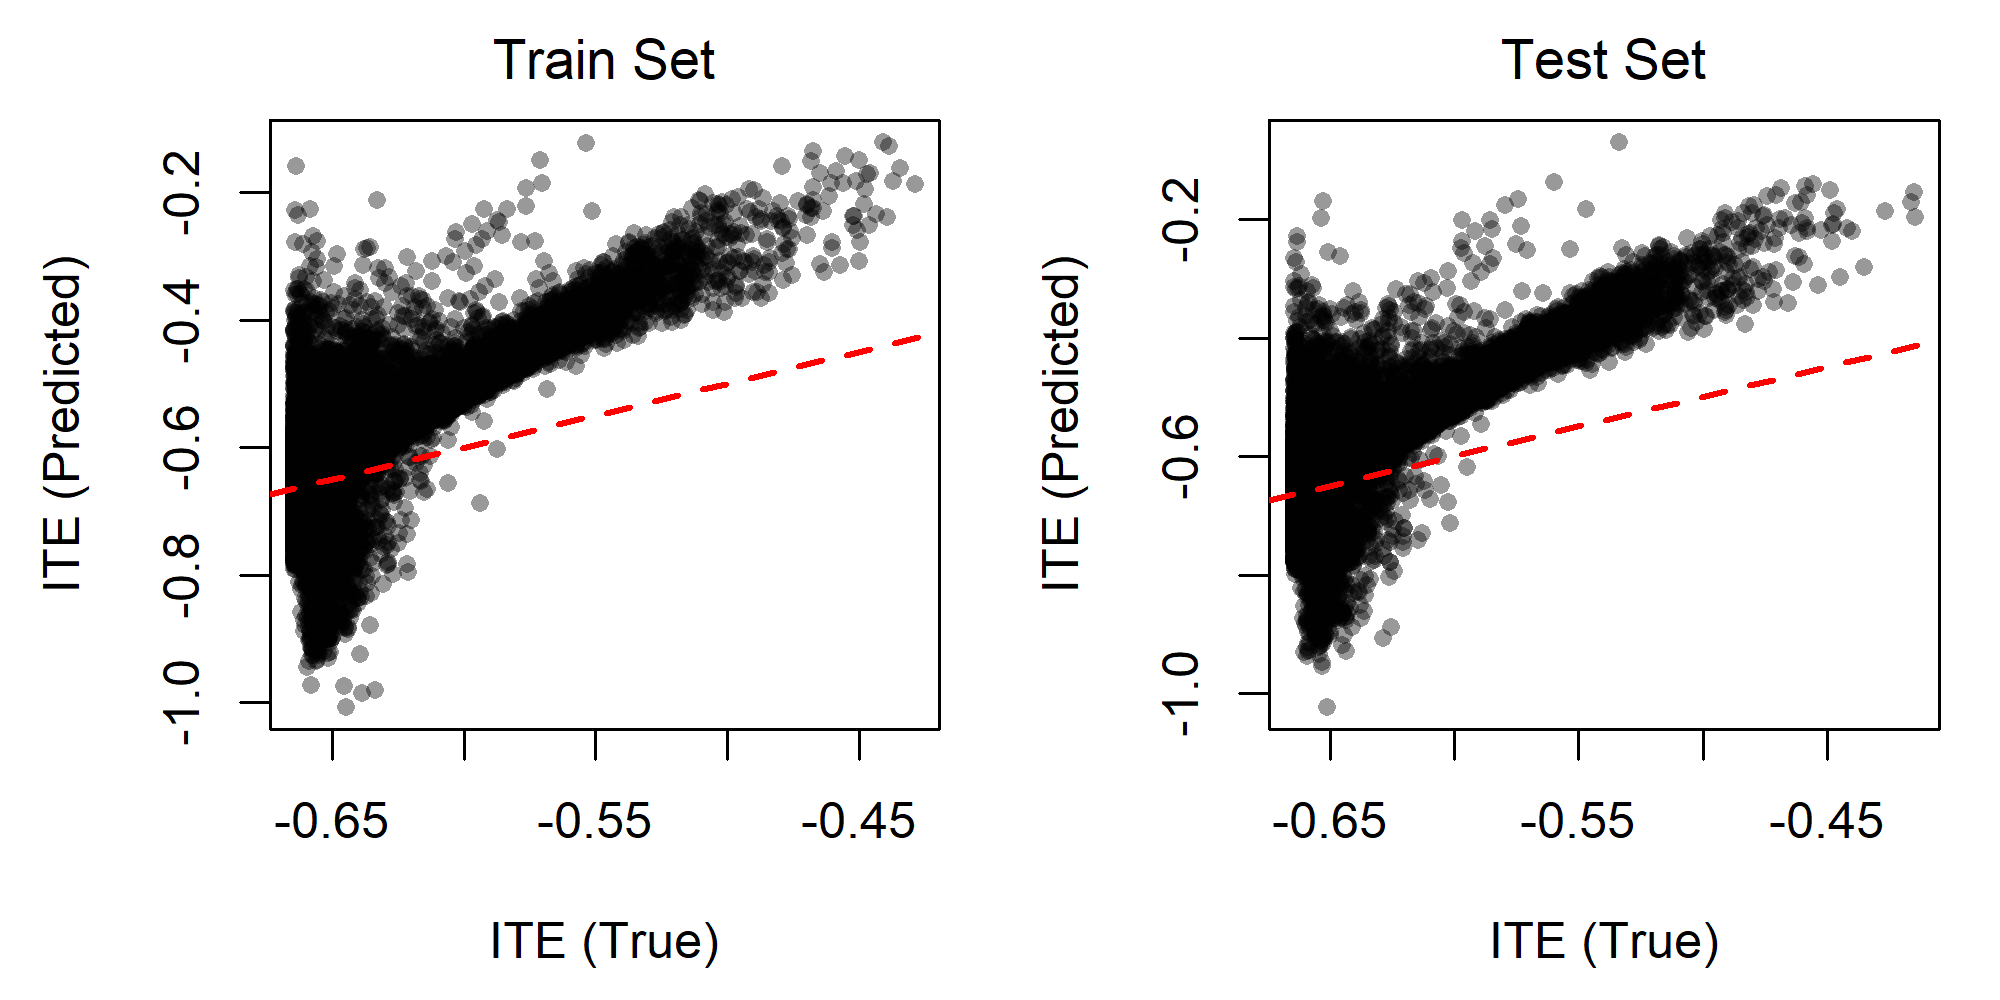
\includegraphics[width=0.45\textwidth]{img/results/rct_scenario2_ITE_scatter_train_test.png}
\caption{Scatterplots of estimated ITEs compared to the true ITEs in the training and test datasets for scenario (2), including a direct treatment but no interaction effects. Left: Observational; right: RCT setting.}
\label{fig:scenario2_ite_scatter_train_test}
\end{figure}




\begin{figure}[htbp]
\centering
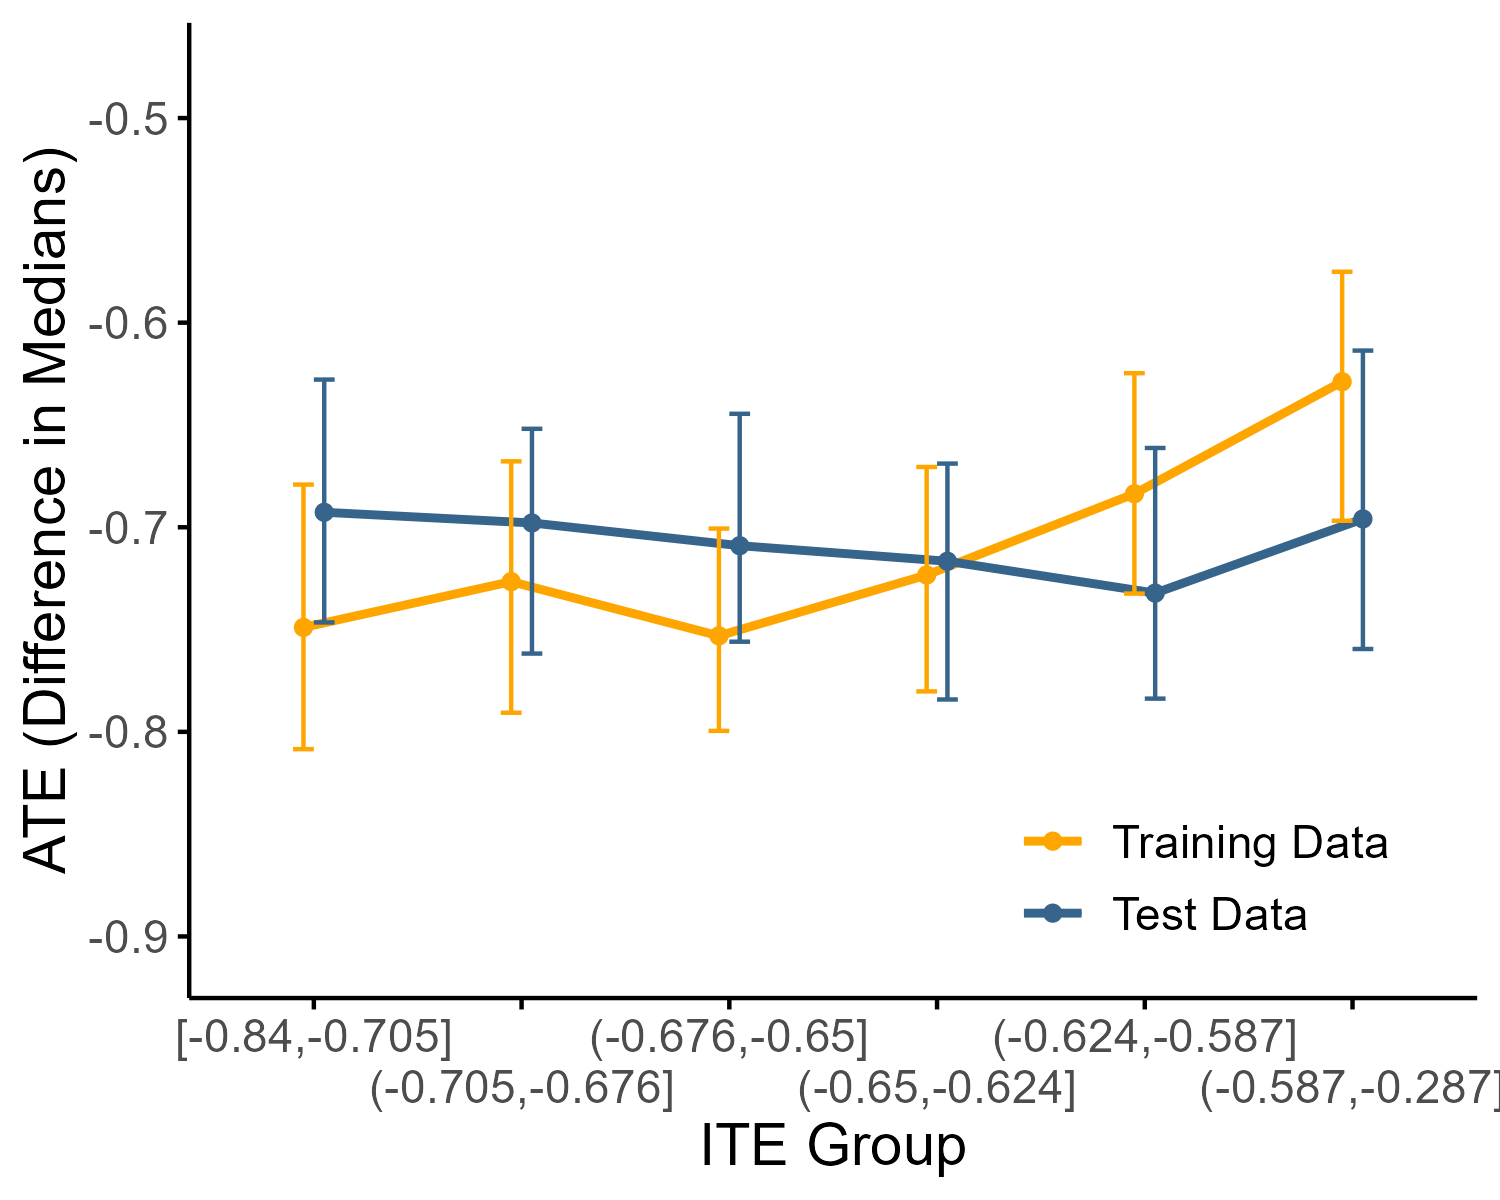
\includegraphics[width=0.45\textwidth]{img/results/observ_scenario2_ITE_cATE.png}
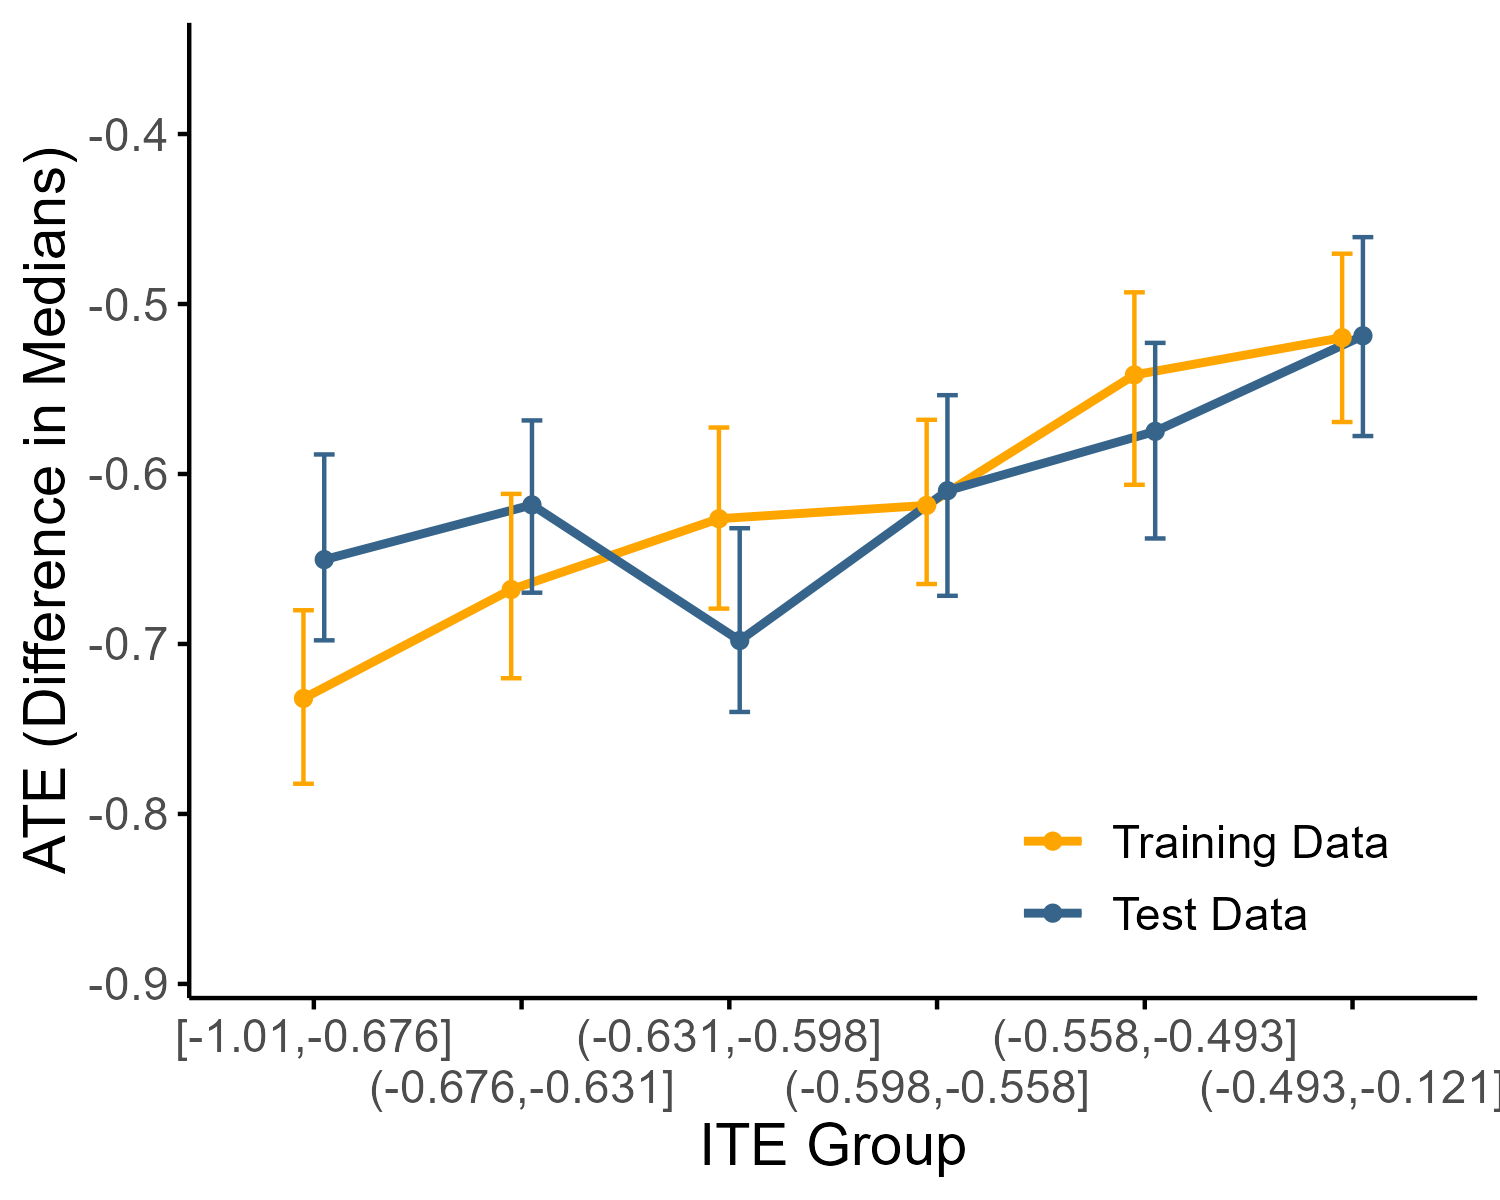
\includegraphics[width=0.45\textwidth]{img/results/rct_scenario2_ITE_cATE.png}
\caption{ITE-ATE plot for scenario (2), including a direct treatment but no interaction effects. Individuals are grouped into bins according to the estimated ITE and in each bin the ATE is calculated as the difference in medians of the observed outcomes under the treatments. 95\% bootstrap confidence intervals indicate the uncertainty. Left: Observational; right: RCT setting.}
\label{fig:scenario2_ite_cATE}
\end{figure}



\clearpage 
¨
\subsection{Scenario (3): No direct but with interaction effects}

Scenario (3) included no direct effect of the treatment on the outcome but it included interaction effects of the treatment with the covariates X2 and X3. Compared to scenario (1), when excluding the direct effect of the treatment, the distribution of ITEs is more centered as shown in Figure \ref{fig:scenario3_ite_distribution_dgp}. The ATE in terms of the mean difference in the test set of the RCT setting is $-0.048$ with a confidence interval of $-0.068$ to $-0.028$. 



\begin{table}[htbp]
\centering
\small
\caption{Scenario (3), without direct treatment effect but including interaction effects: Comparison of ATE measures across train and test sets for the observational and RCT setting.}
\label{tab:scenario3_ate_comparison}
\begin{tabular}{l c c c c}
\toprule
\textbf{Measure} & \multicolumn{2}{c}{\textbf{Observational}} & \multicolumn{2}{c}{\textbf{RCT}} \\
\cmidrule(lr){2-3} \cmidrule(lr){4-5}
 & \textbf{Train} & \textbf{Test} & \textbf{Train} & \textbf{Test} \\
\midrule
ATE as $\text{mean}(\text{Y}_\text{observed}^{(1)}) - \text{mean}(\text{Y}_\text{observed}^{(0)})$ & NA & NA & -0.048 & -0.048 \\
ATE as $\text{median}(\text{Y}_\text{observed}^{(1)}) - \text{median}(\text{Y}_\text{observed}^{(0)})$ & NA & NA & -0.048 & -0.059 \\
ATE as mean(ITE$_\text{true}$)  & -0.065 & -0.068 & -0.065 & -0.068 \\
ATE as mean(ITE$_\text{estimated}$) & -0.059 & -0.061 & -0.051 & -0.053 \\
\bottomrule
\end{tabular}
\end{table}



\begin{figure}[htbp]
\centering
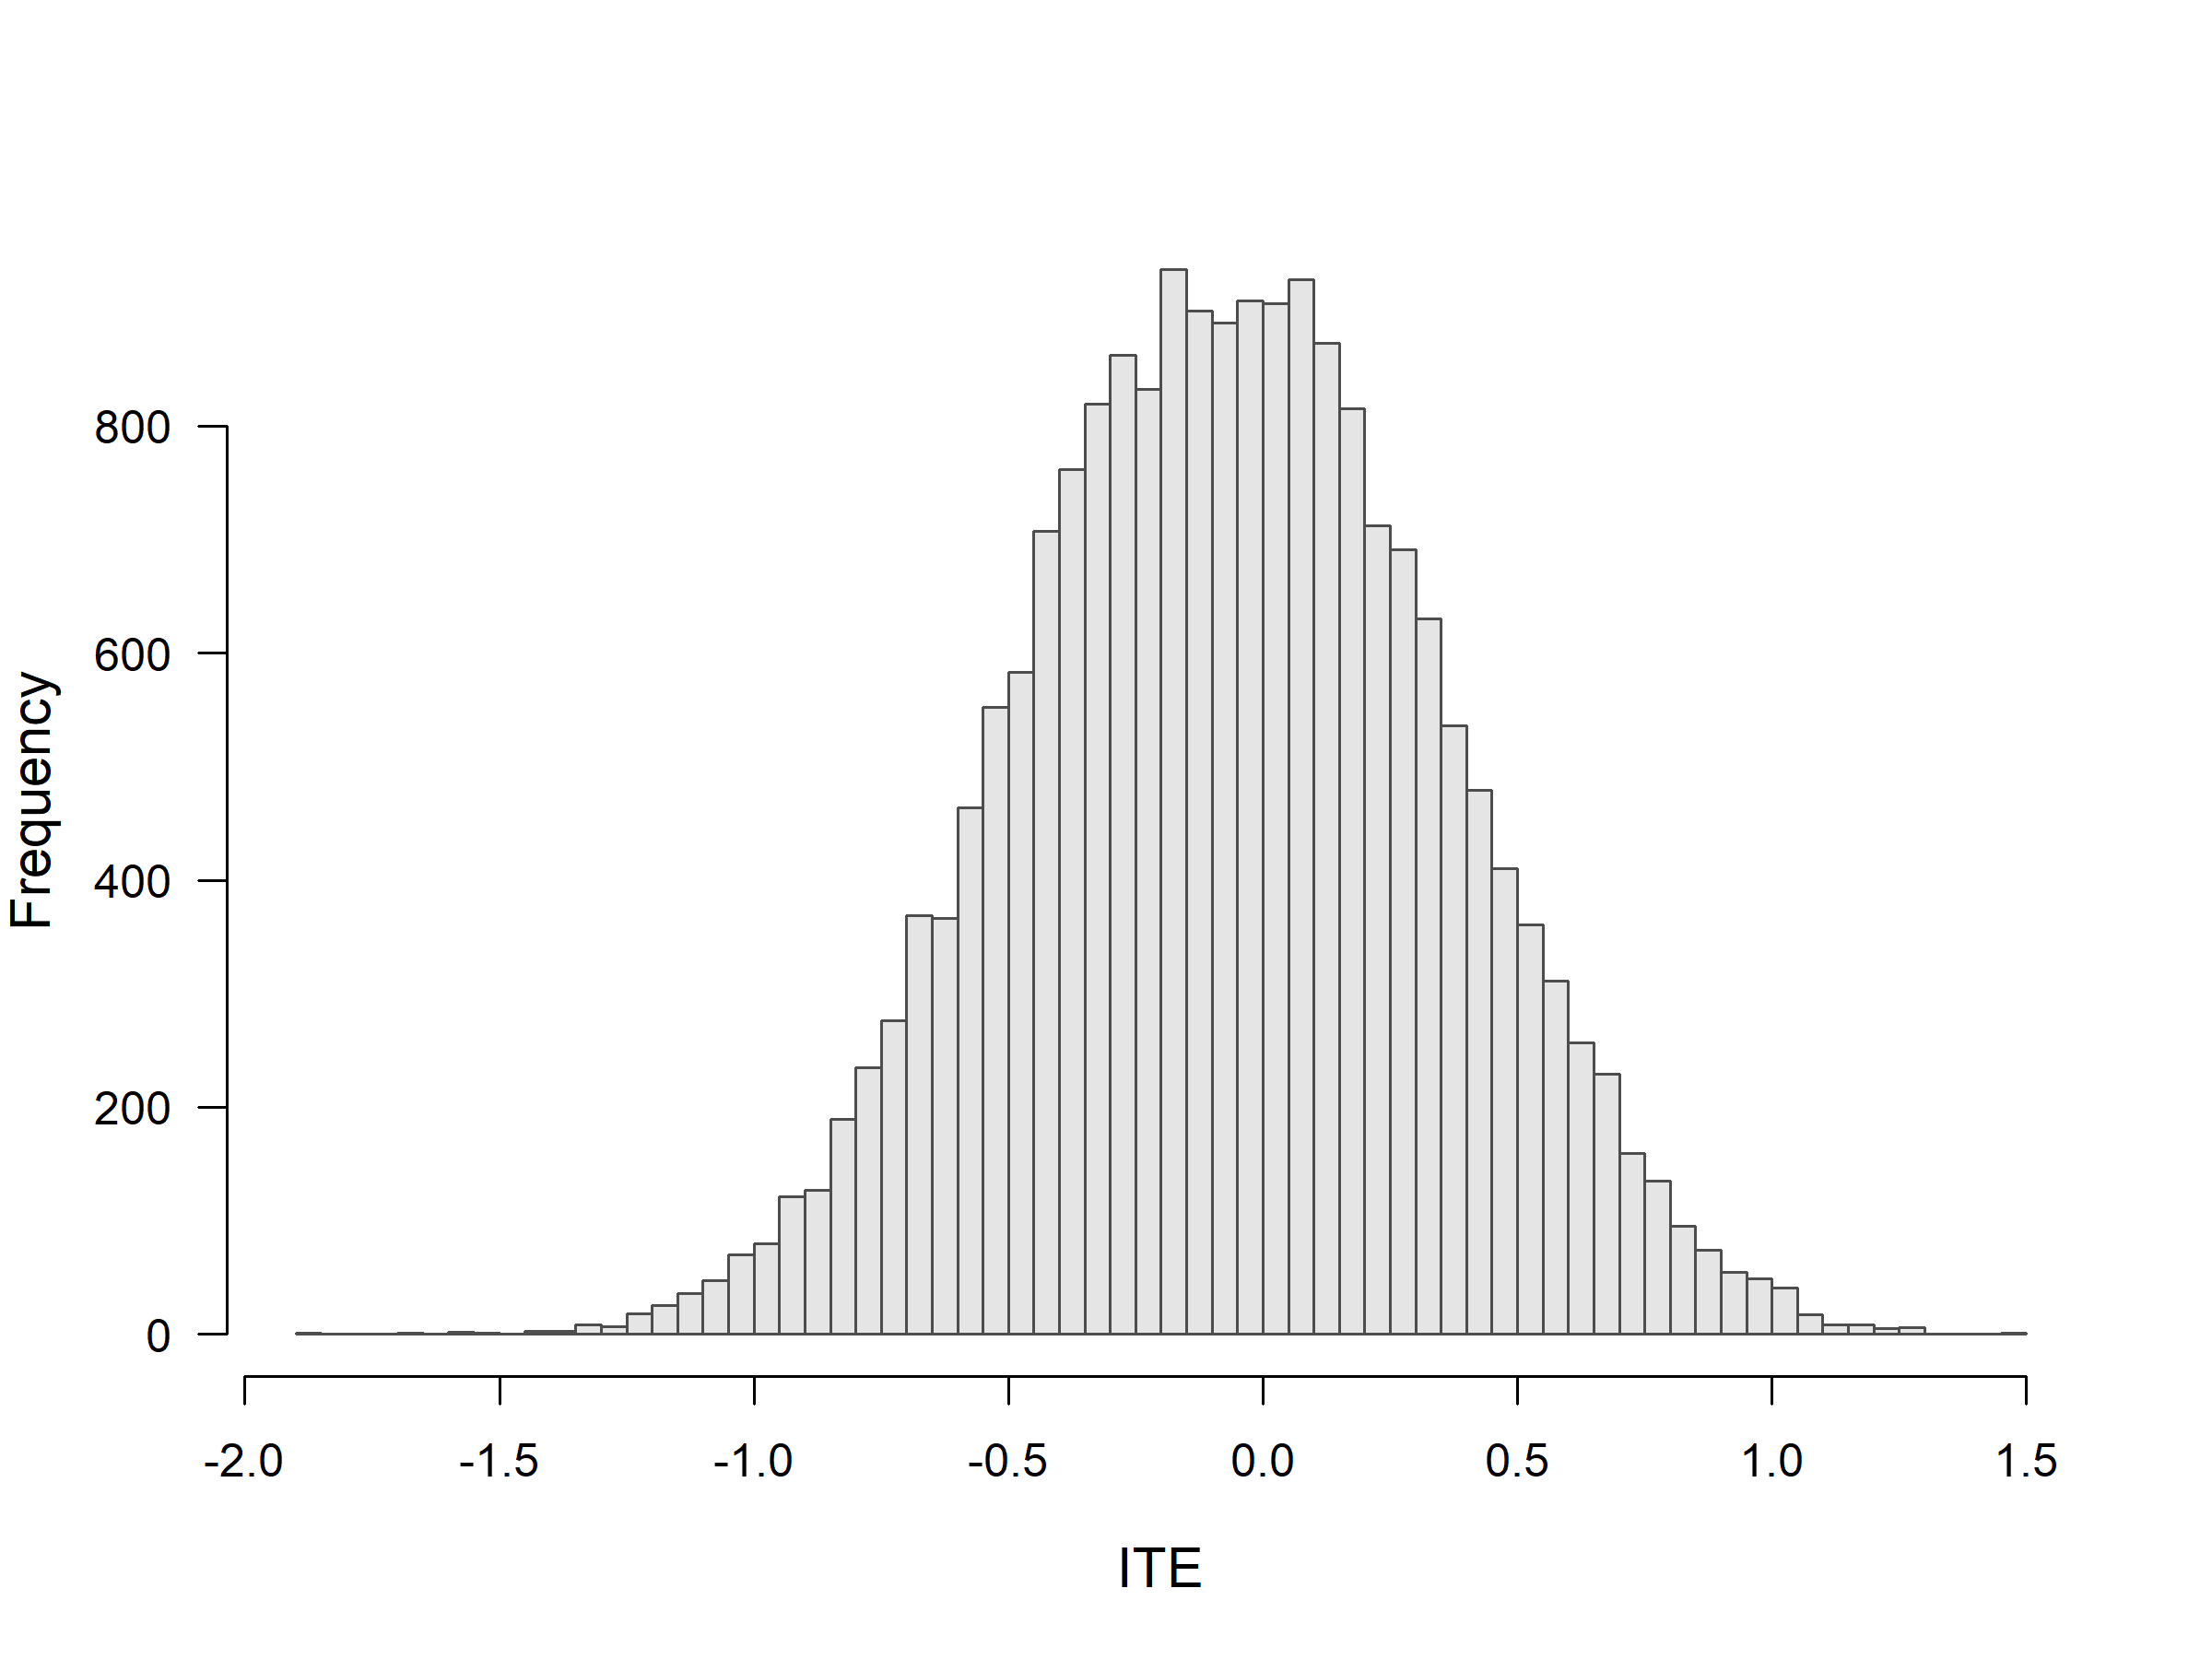
\includegraphics[width=0.45\textwidth]{img/results/observ_scenario3_ite_distribution_dgp.png}
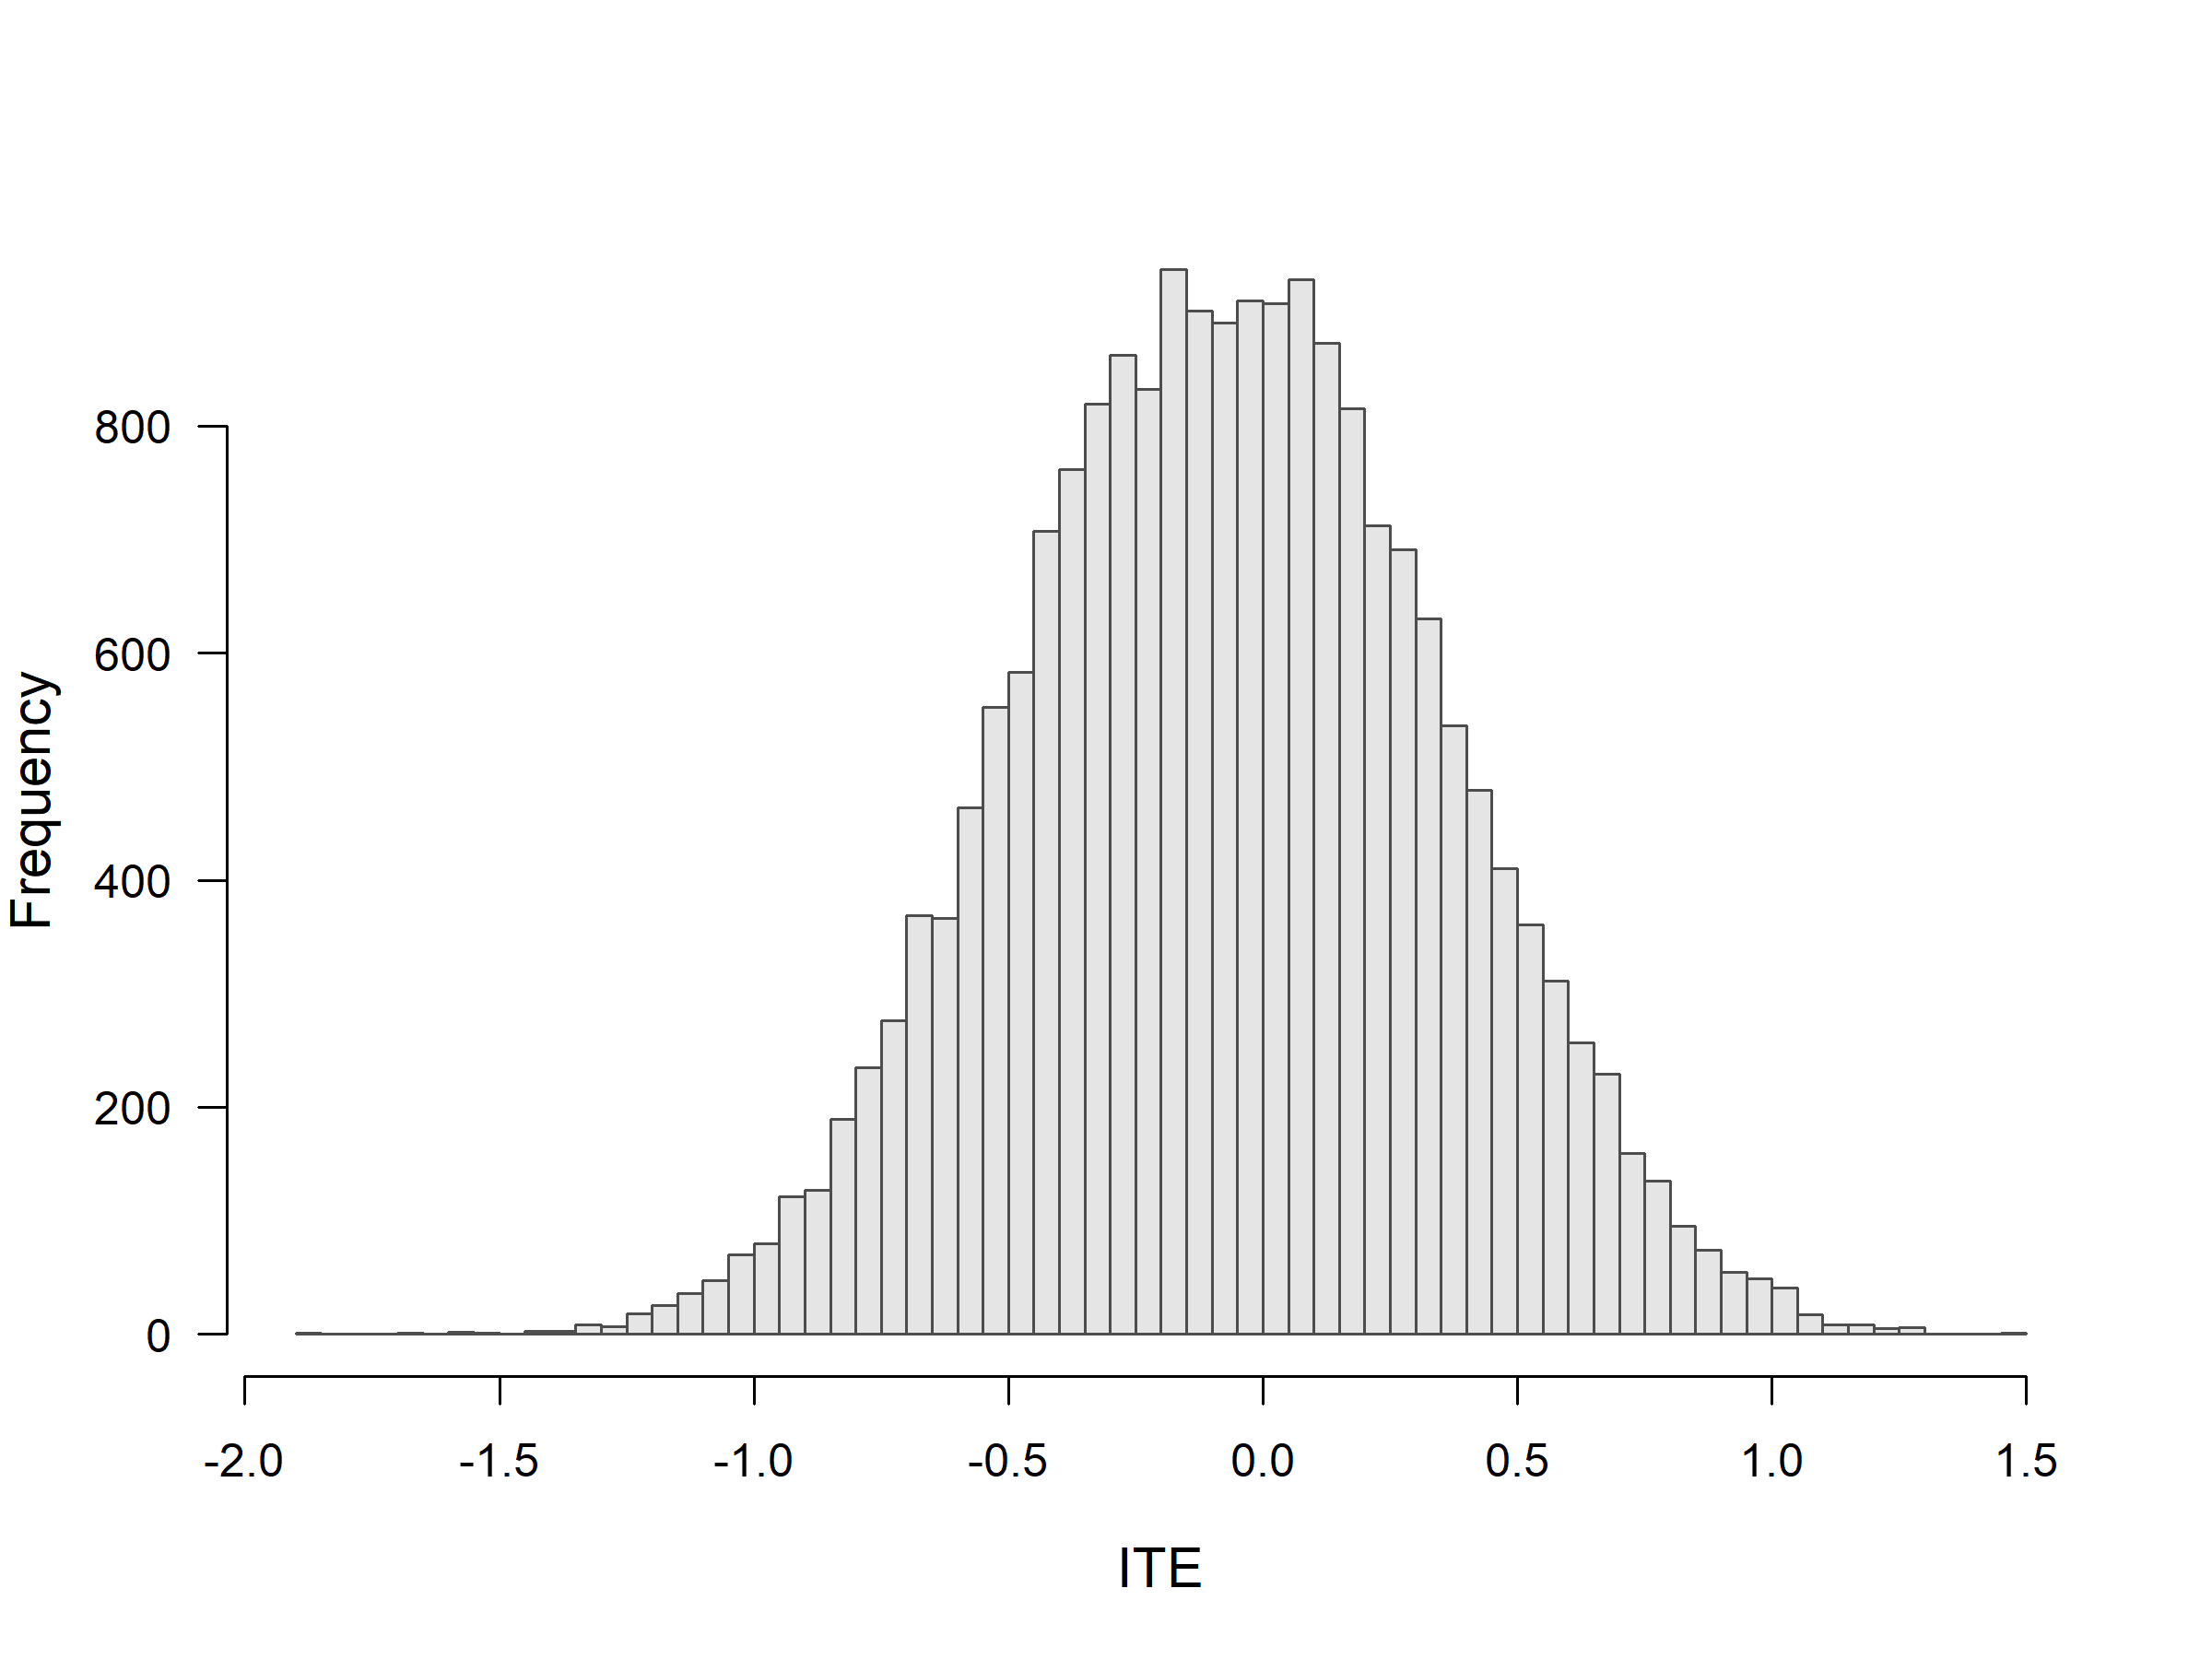
\includegraphics[width=0.45\textwidth]{img/results/rct_scenario3_ite_distribution_dgp.png}
\caption{True ITE distribution resulting from the DGP for scenario (3), without direct treatment effect but including interaction effects. The true ITEs are identical in the observational and in the RCT setting, since they depend on the potential outcomes under both treatment allocations. Left: Observational; Right: RCT setting.}
\label{fig:scenario3_ite_distribution_dgp}
\end{figure}



\begin{figure}[htbp]
\centering
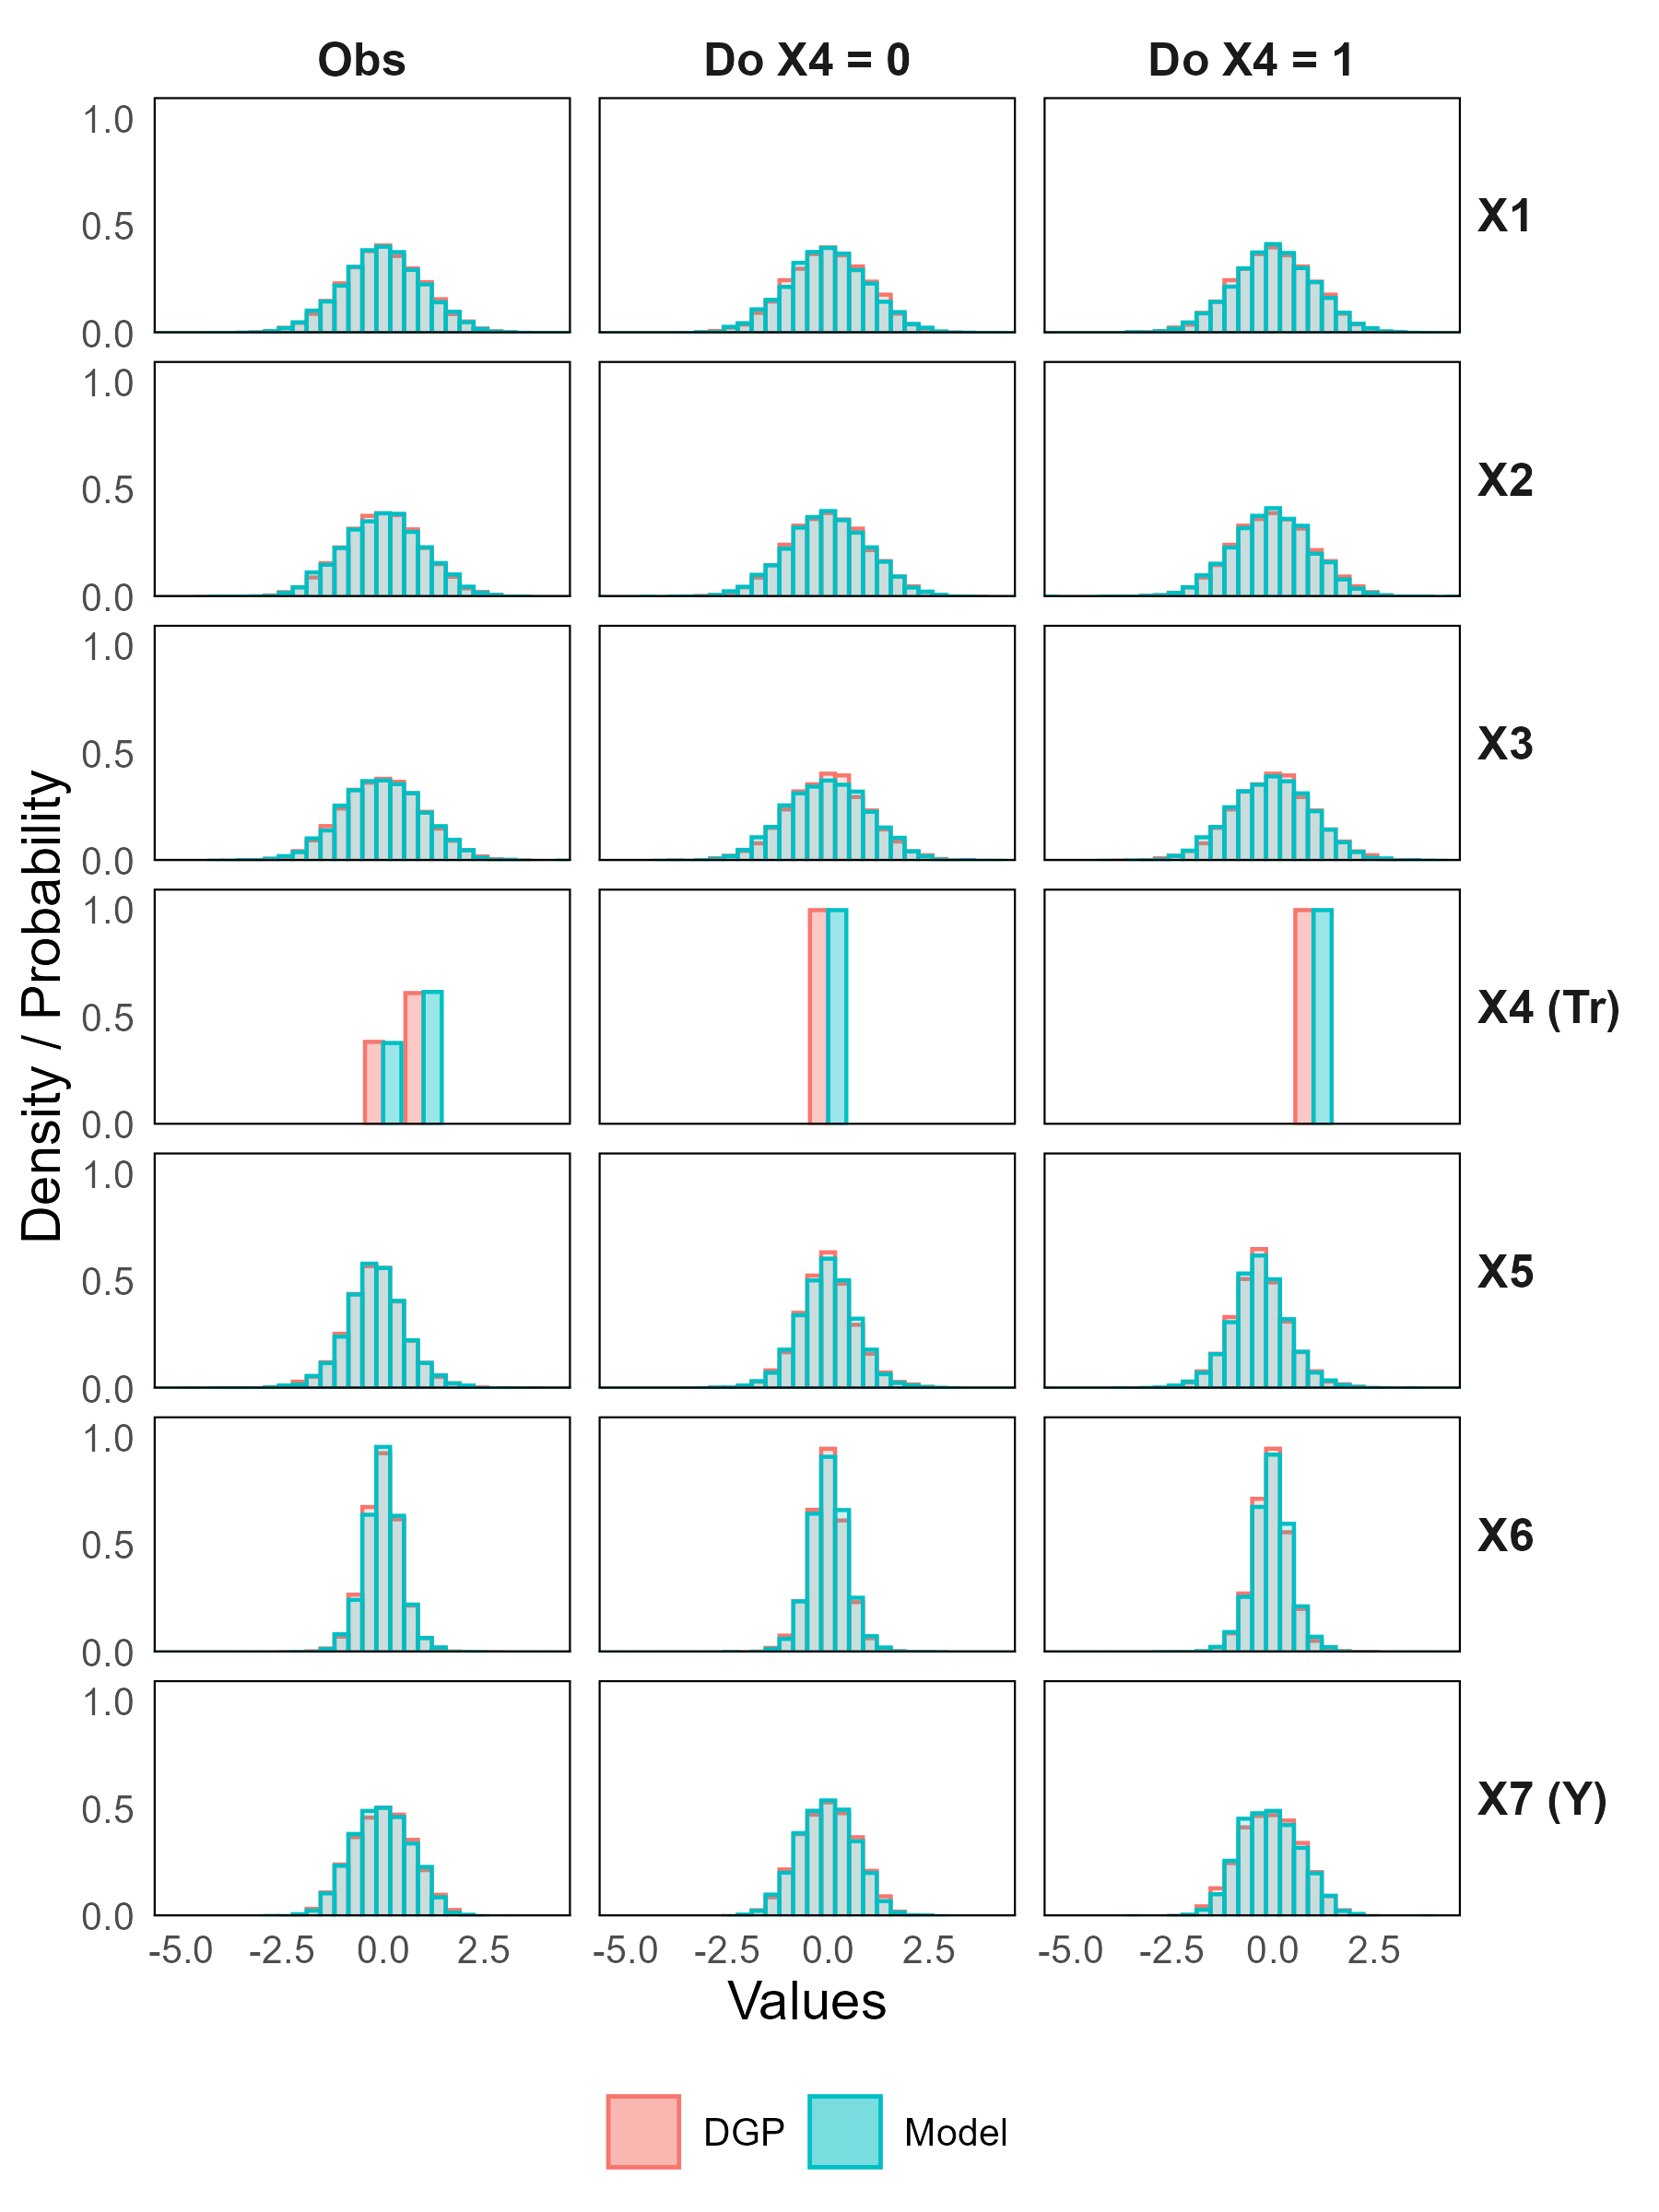
\includegraphics[width=0.45\textwidth]{img/results/observ_scenario3_sampling_distributions_vertical.png}
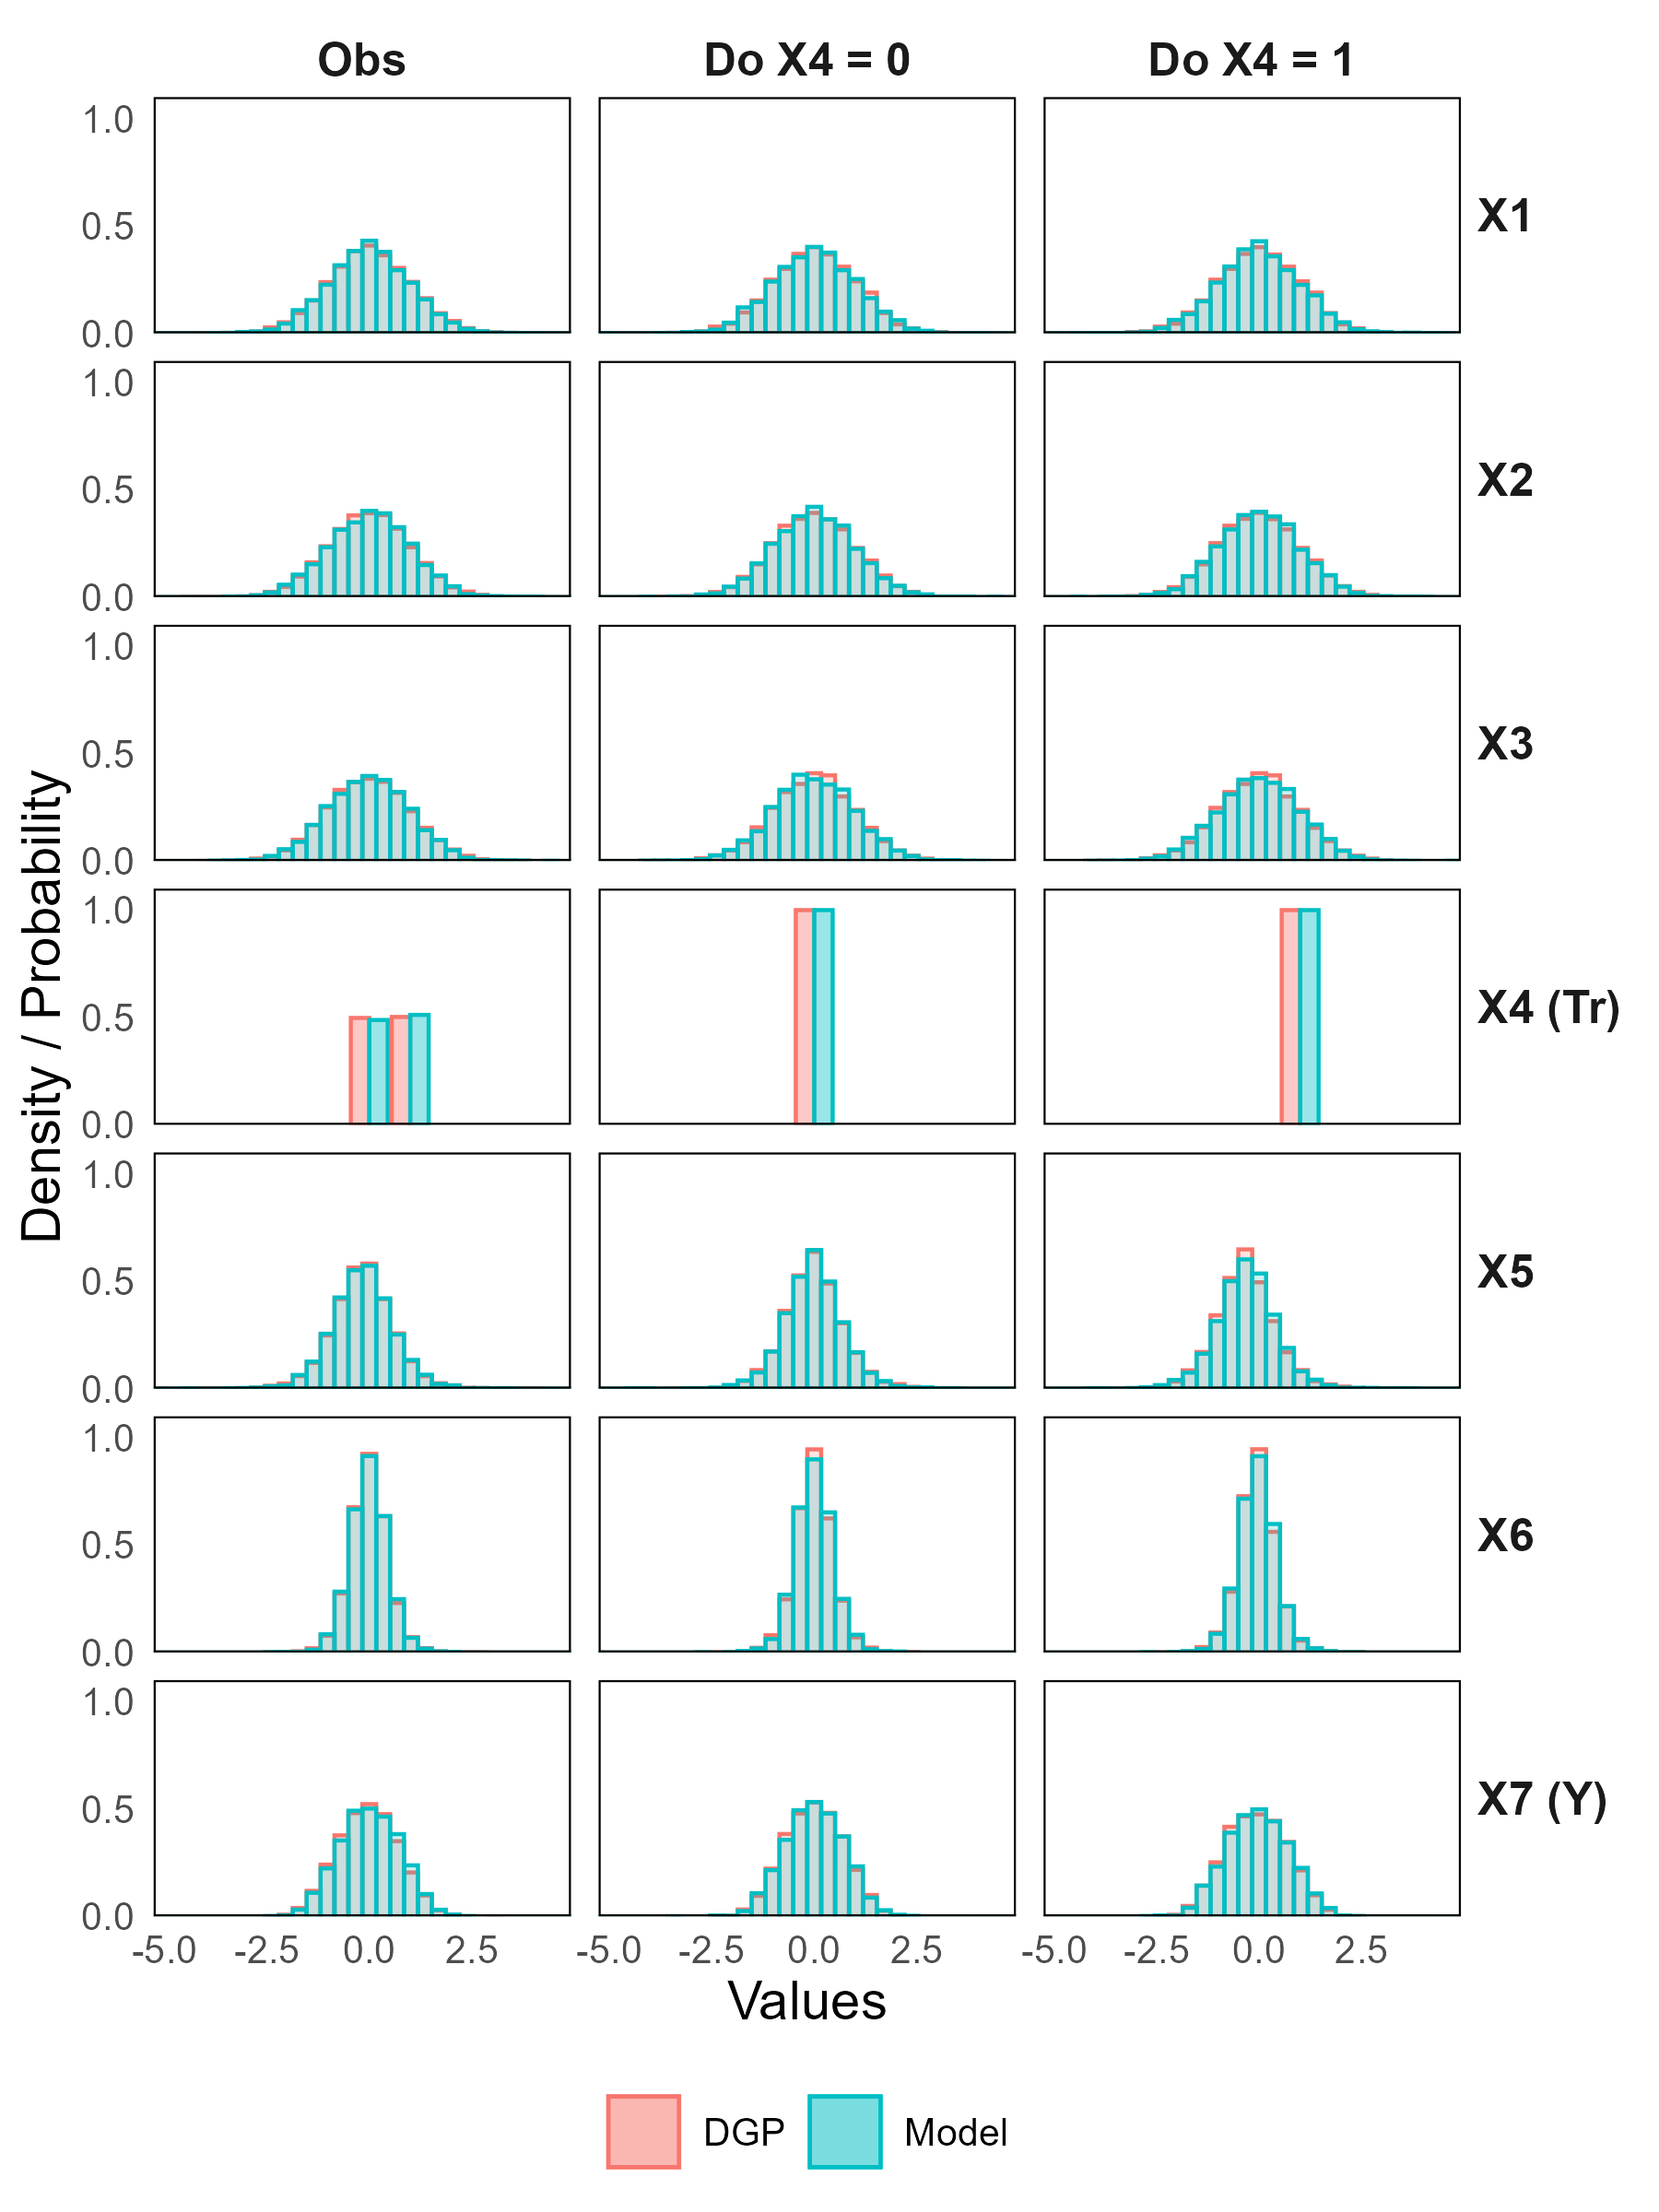
\includegraphics[width=0.45\textwidth]{img/results/rct_scenario3_sampling_distributions_vertical.png}
\caption{Marginal distributions of DGP variables and fitted TRAM-DAG samples for scenario (3), without direct treatment effect but including interaction effects. The distributions shown as observed (Obs), under control intervention (Do $X4=0$) and under treatment intervention (Do $X4=1$). Left: Observational; Right: RCT setting.}
\label{fig:scenario3_sampling_distributions_vertical}
\end{figure}

\begin{figure}[htbp]
\centering
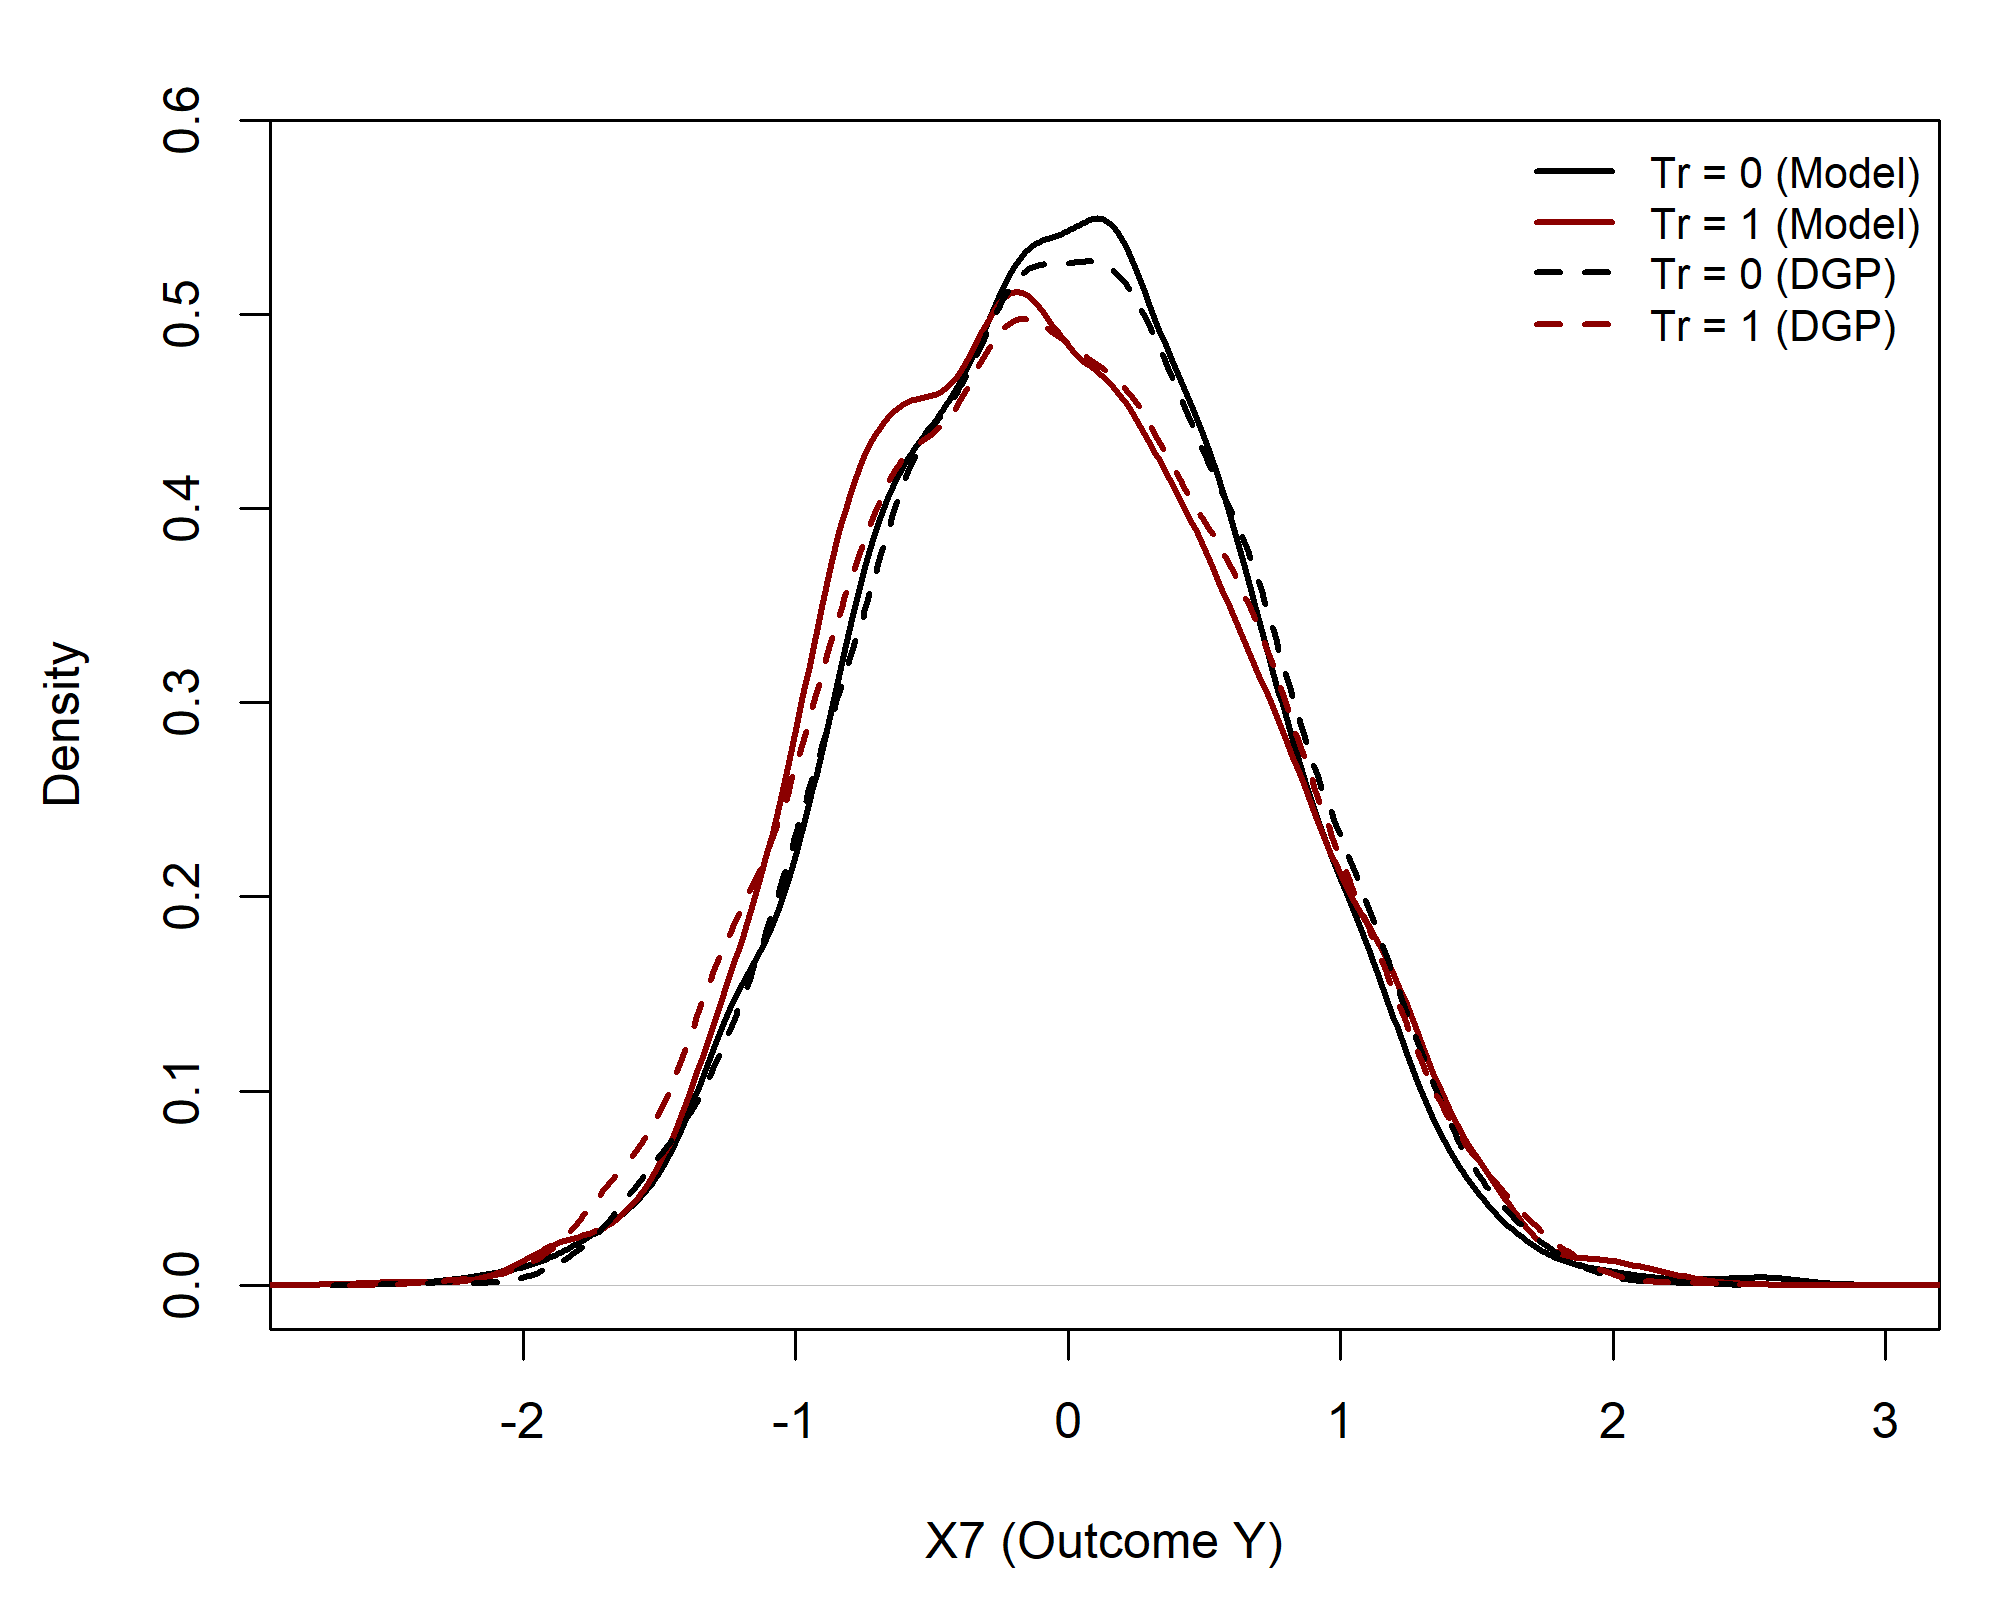
\includegraphics[width=0.45\textwidth]{img/results/observ_scenario3_X7_treatment_densities.png}
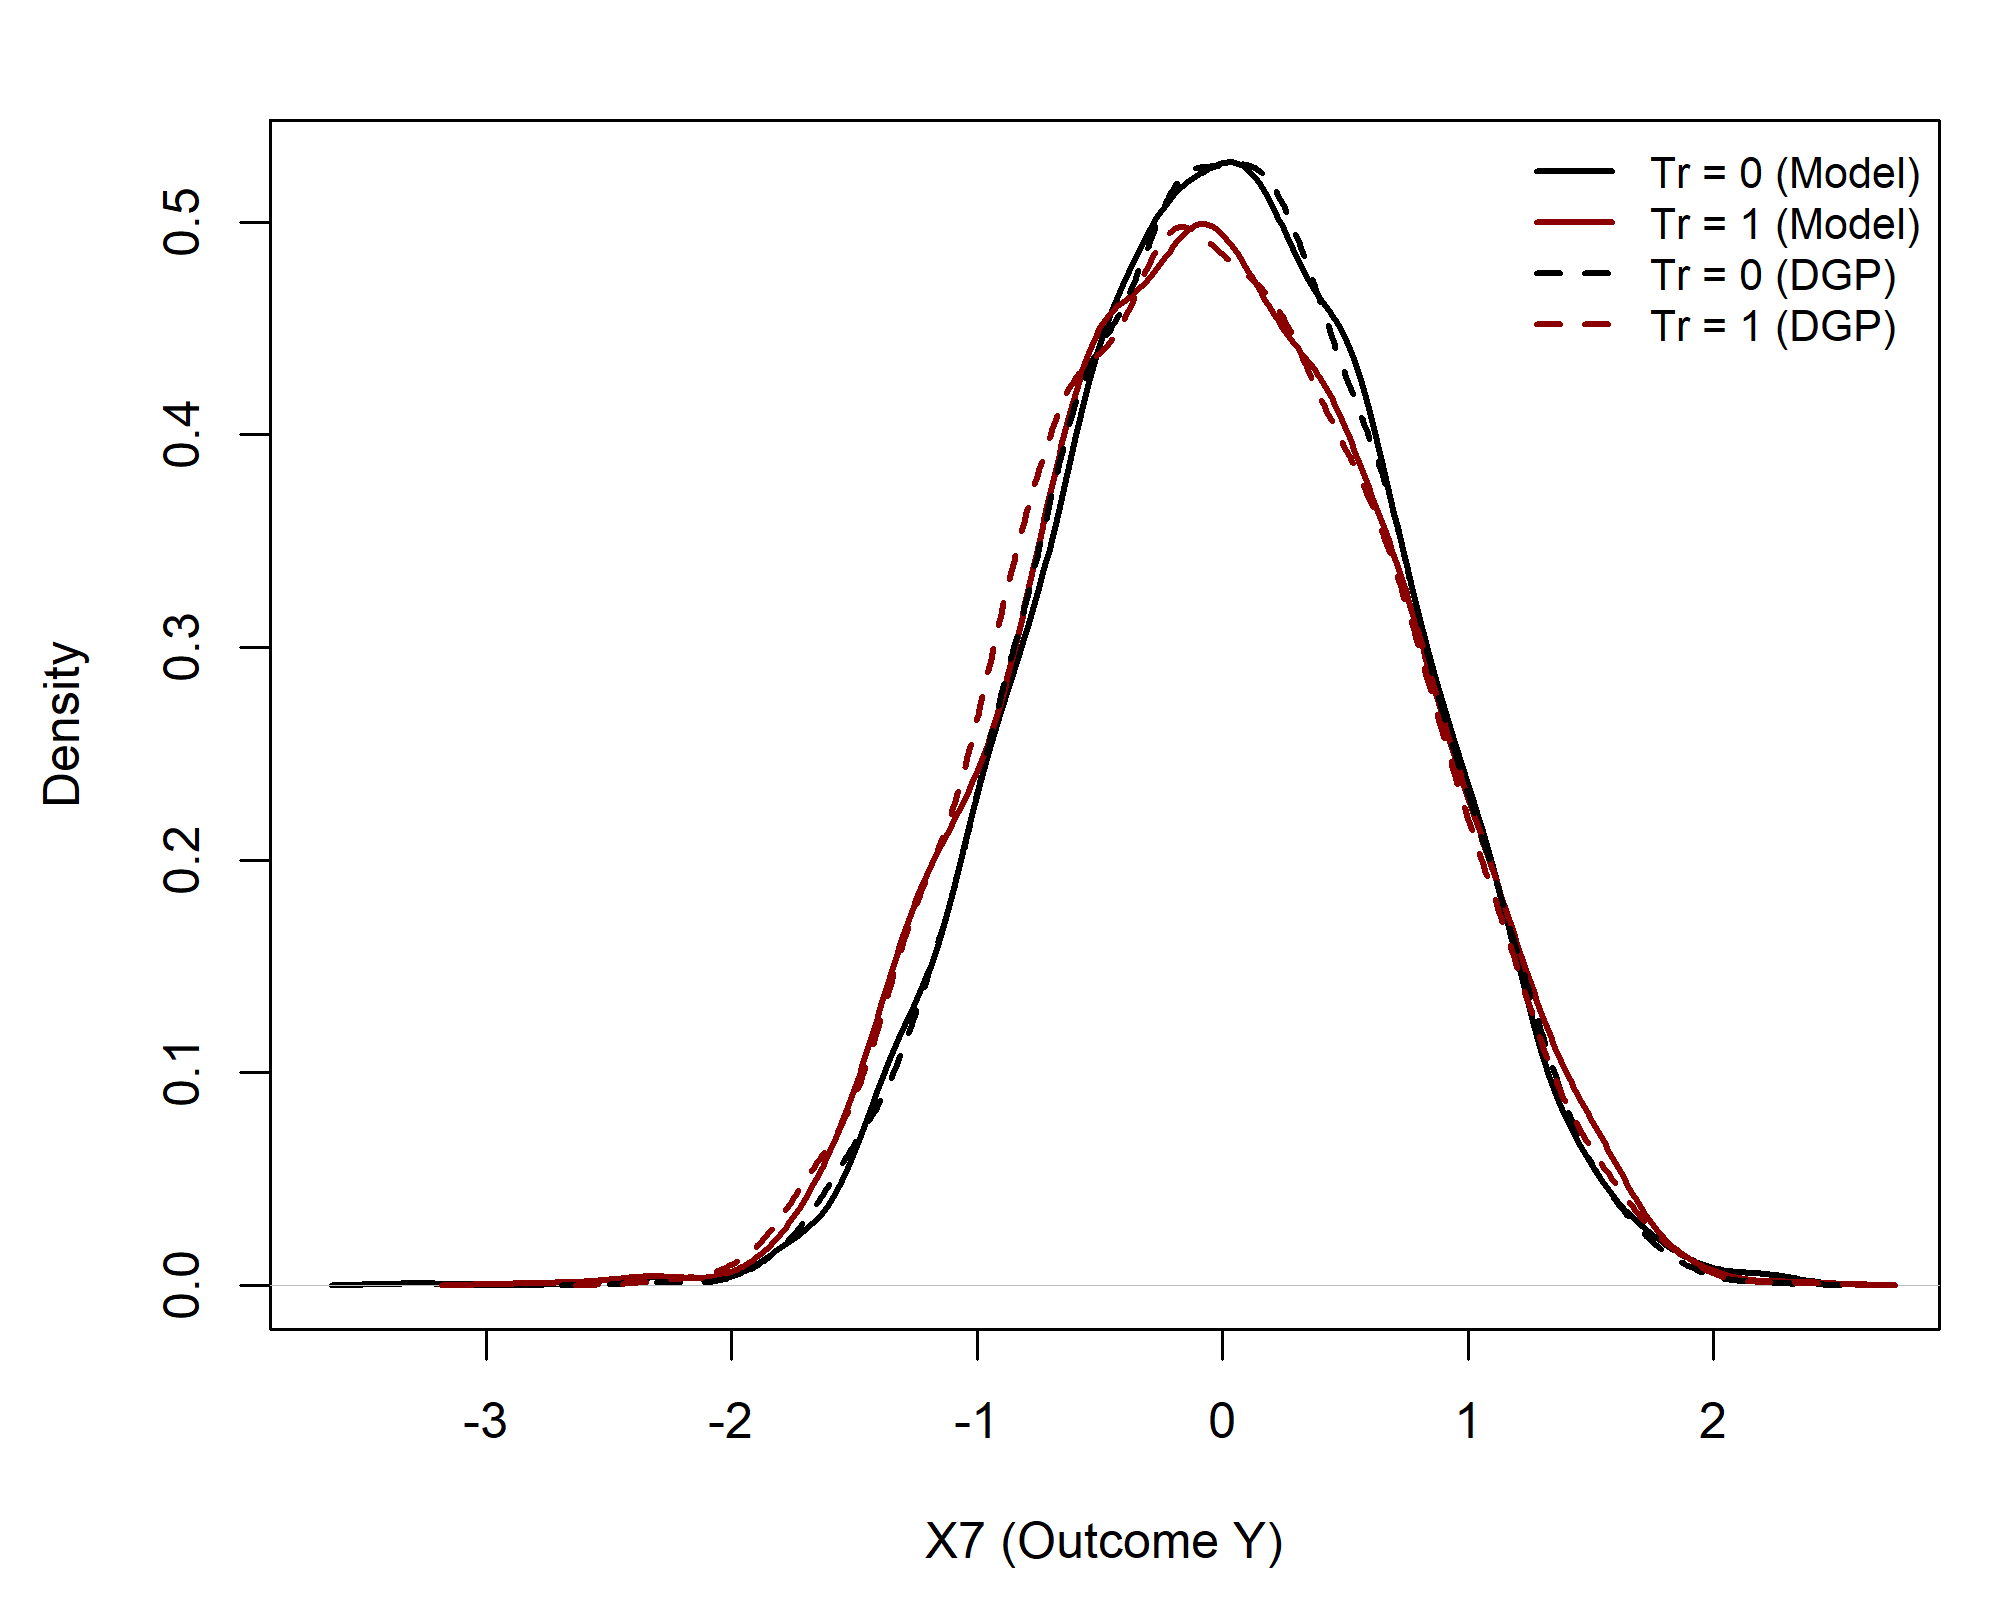
\includegraphics[width=0.45\textwidth]{img/results/rct_scenario3_X7_treatment_densities.png}
\caption{Distributions of the outcome variable (X7) under treatment and control interventions for scenario (3), without direct treatment effect but including interaction effects. This plot is a higher resolution view of the X7 panels (Do $X4=0$) and (Do $X4=1$) from Figure \ref{fig:scenario3_sampling_distributions_vertical}. Left: Observational; Right: RCT setting.}
\label{fig:scenario3_outcome_distributions}
\end{figure}




\begin{figure}[htbp]
\centering
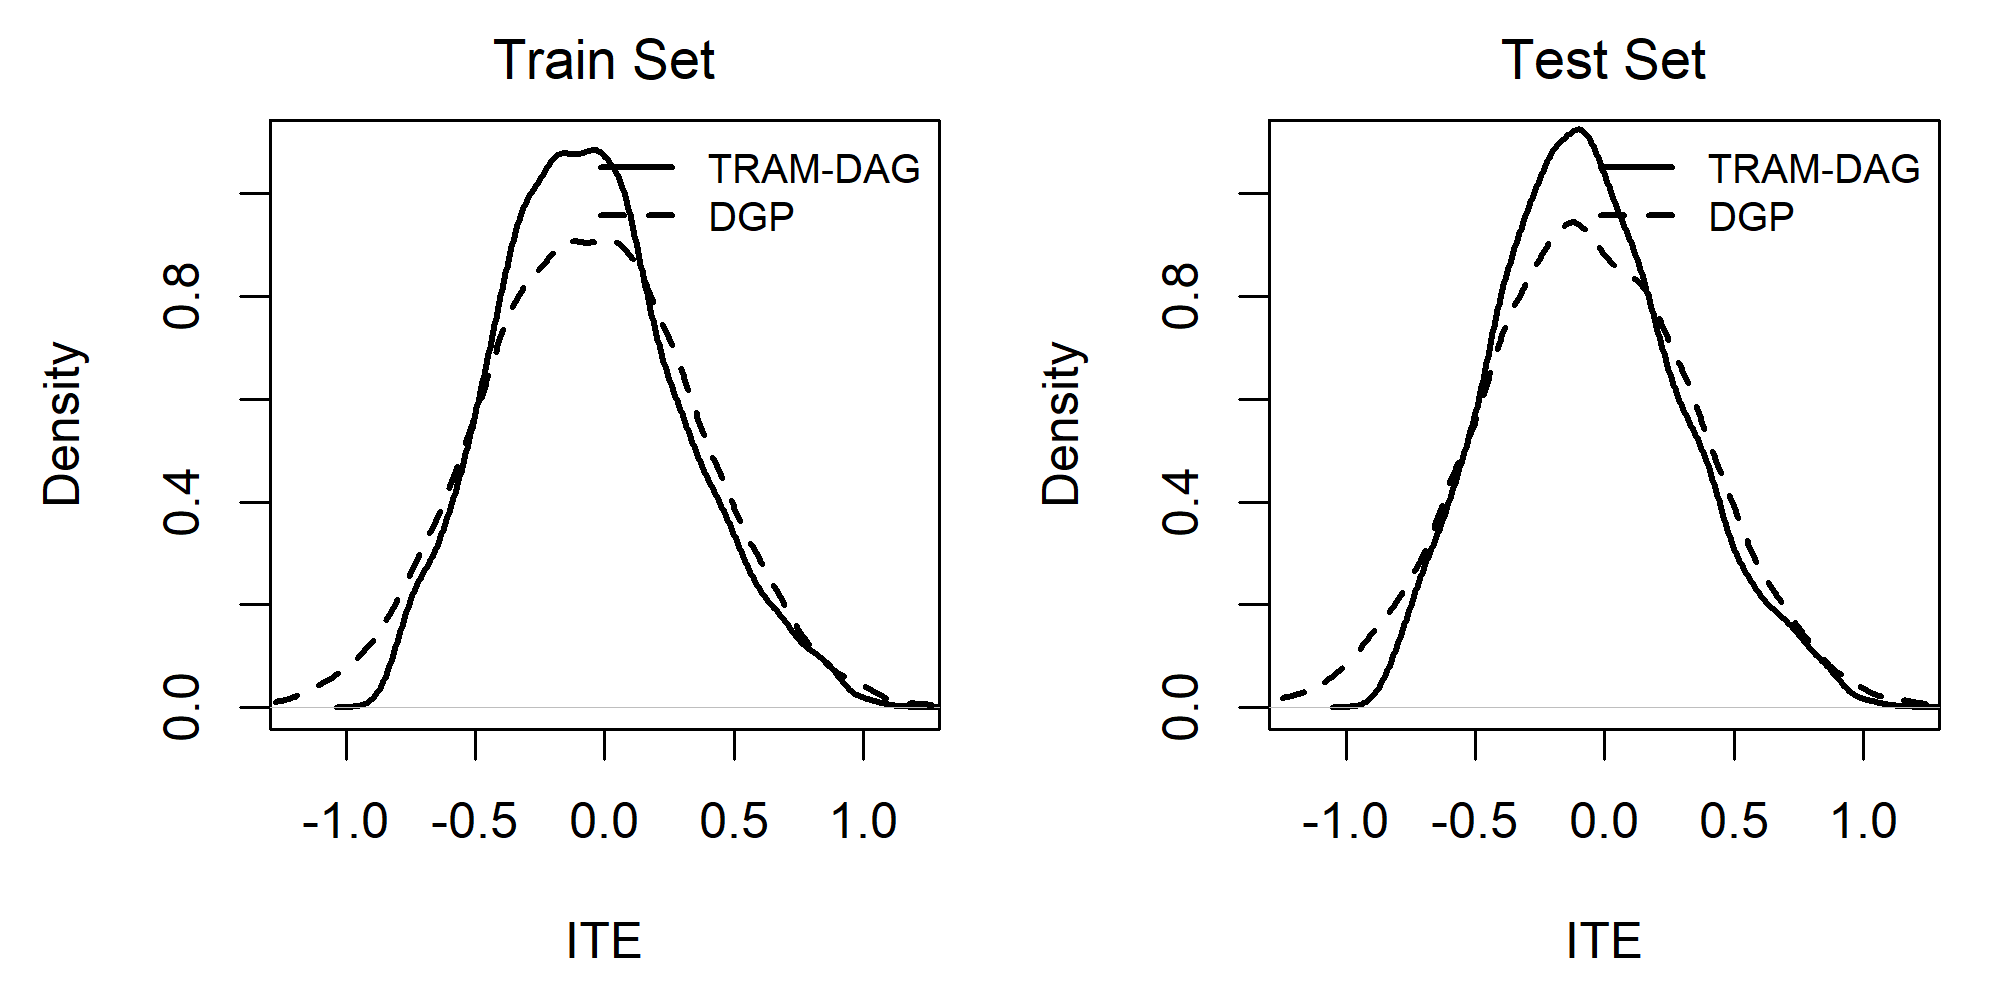
\includegraphics[width=0.45\textwidth]{img/results/observ_scenario3_ITE_densities_train_test.png}
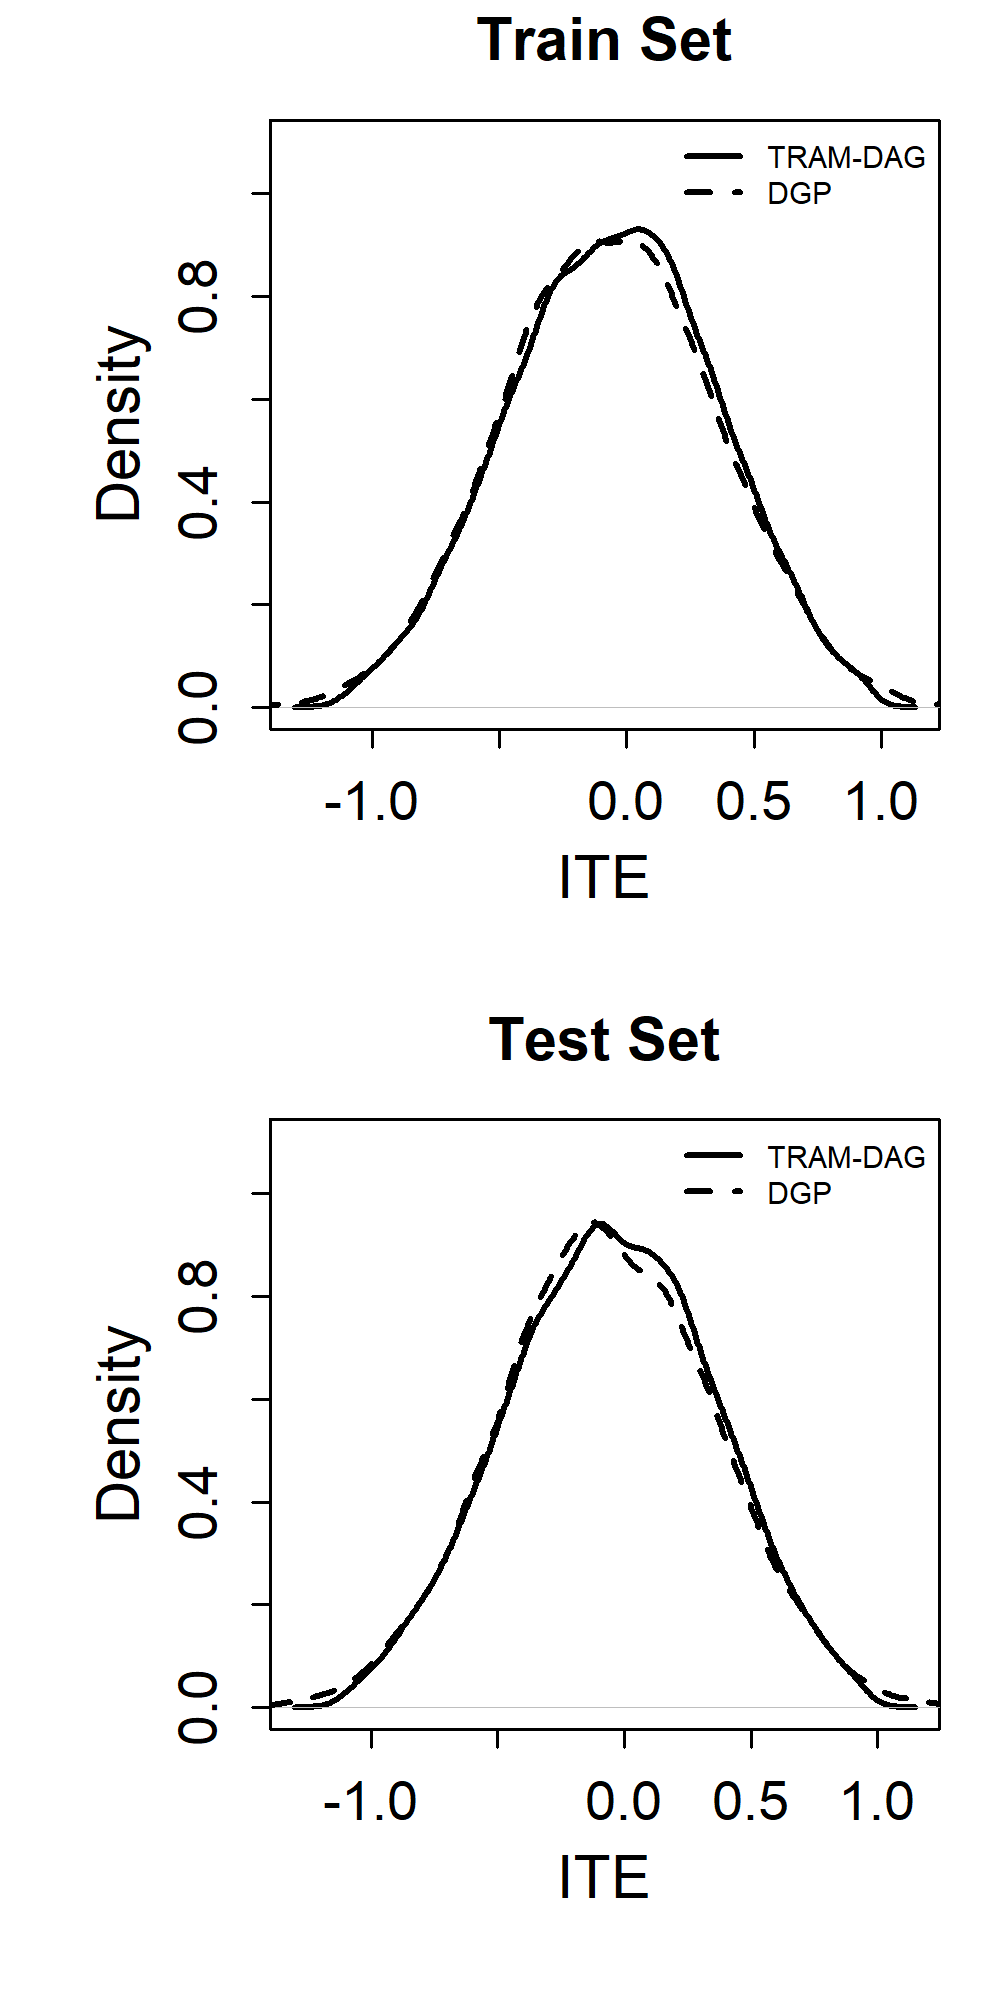
\includegraphics[width=0.45\textwidth]{img/results/rct_scenario3_ITE_densities_train_test.png}
\caption{Densities of estimated ITEs compared to the true ITEs in the training and test datasets for scenario (3), without direct treatment effect but including interaction effects. Left: Observational; right: RCT setting.}
\label{fig:scenario3_ite_densities_train_test}
\end{figure}






\begin{figure}[htbp]
\centering
\includegraphics[width=0.45\textwidth]{img/results/observ_scenario3_ITE_scatter_train_test.png}
\includegraphics[width=0.45\textwidth]{img/results/rct_scenario3_ITE_scatter_train_test.png}
\caption{Scatterplots of estimated ITEs compared to the true ITEs in the training and test datasets for scenario (3), without direct treatment effect but including interaction effects. Left: Observational; right: RCT setting.}
\label{fig:scenario3_ite_scatter_train_test}
\end{figure}




\begin{figure}[htbp]
\centering
\includegraphics[width=0.45\textwidth]{img/results/observ_scenario3_ITE_cATE.png}
\includegraphics[width=0.45\textwidth]{img/results/rct_scenario3_ITE_cATE.png}
\caption{ITE-ATE plot for scenario (3), without direct treatment effect but including interaction effects. Individuals are grouped into bins according to the estimated ITE and in each bin the ATE is calculated as the difference in medians of the observed outcomes under the treatments. 95\% bootstrap confidence intervals indicate the uncertainty. Left: Observational; right: RCT setting.}
\label{fig:scenario3_ite_cATE}
\end{figure}


